\documentclass[12pt]{article}

%VARIABLES
\def \geometryDefault {
	a4paper,
	left=35mm,
	right=20mm,
	top=25mm,
	bottom=25mm
}
\def \geometryTitlePage {
	left=25mm,
	right=25mm,
	top=25mm,
	bottom=25mm
}
\def \geometryGraduationCard {
	left=25mm,
	right=10mm,
	top=25mm,
	bottom=25mm
}
\def \geometryStatement {
	left=25mm,
	right=10mm,
	top=25mm,
	bottom=25mm
}


%page settings
\usepackage{float}
\usepackage[\geometryDefault]{geometry}% margins
\usepackage{times} % Times New Roman
\setlength{\parindent}{1cm} % tab indentation
\linespread{1.5} % interline
\usepackage{indentfirst} % tab the first line in a section

%language settings
\usepackage[utf8]{inputenc}
\usepackage[T1]{fontenc}
\usepackage[polish]{babel}
\usepackage{csquotes}
\DeclareQuoteAlias{croatian}{polish} % croatian has the same properties as polish
\usepackage[final]{pdfpages}

%code options
\usepackage{listings}
\usepackage{xcolor}

\colorlet{punct}{red!60!black}
\definecolor{delim}{RGB}{20,105,176}
\colorlet{numb}{magenta!60!black}

\lstdefinelanguage{json}{
    basicstyle=\normalfont\ttfamily,
    %numbers=left,
    numberstyle=\scriptsize,
    stepnumber=1,
    frame=single,
    %showstringspaces=false,
    breaklines=true,
    captionpos=b,
    escapeinside={\%*}{*)},
    literate={ą}{{\k{a}}}1
             {Ą}{{\k{A}}}1
             {ę}{{\k{e}}}1
             {Ę}{{\k{E}}}1
             {ó}{{\'o}}1
             {Ó}{{\'O}}1
             {ś}{{\'s}}1
             {Ś}{{\'S}}1
             {ł}{{\l{}}}1
             {Ł}{{\L{}}}1
             {ż}{{\.z}}1
             {Ż}{{\.Z}}1
             {ź}{{\'z}}1
             {Ź}{{\'Z}}1
             {ć}{{\'c}}1
             {Ć}{{\'C}}1
             {ń}{{\'n}}1
             {Ń}{{\'N}}1
}

\lstdefinelanguage{swift}
{
  morekeywords={
    try,func,if,then,else,for,in,while,do,switch,case,default,where,break,continue,fallthrough,return,
    typealias,struct,class,enum,protocol,var,func,let,get,set,willSet,didSet,inout,init,deinit,extension,
    subscript,prefix,operator,infix,postfix,precedence,associativity,left,right,none,convenience,dynamic,
    final,lazy,mutating,nonmutating,optional,override,required,static,unowned,safe,weak,internal,
    private,public,is,as,self,unsafe,dynamicType,true,false,nil,Type,Protocol,
  },
  morecomment=[l]{//}, % l is for line comment
  morecomment=[s]{/*}{*/}, % s is for start and end delimiter
  morestring=[b]" % defines that strings are enclosed in double quotes
}

\definecolor{keyword}{HTML}{BA2CA3}
\definecolor{string}{HTML}{D12F1B}
\definecolor{comment}{HTML}{008400}

\lstset{
  language=swift,
  basicstyle=\ttfamily,
  showstringspaces=false, % lets spaces in strings appear as real spaces
  columns=fixed,
  keepspaces=true,
  keywordstyle=\color{keyword},
  stringstyle=\color{string},
  commentstyle=\color{comment},
}

\renewcommand\lstlistingname{Kod źródłowy}
\renewcommand{\lstlistlistingname}{Kody źródłowe}

\AtBeginDocument{%
  \renewcommand\tablename{Tabela}
  \renewcommand\listtablename{Spis tabel}
}

%Here I change numeric pattern to include chapter number
\usepackage{chngcntr}
\AtBeginDocument{\counterwithin{lstlisting}{section}} %listings
\AtBeginDocument{\counterwithin{figure}{section}} %images

%Make images captions to be on the bottom
%\usepackage{floatrow}

%Define new block, so that if a code is split between 2 pages, then it moves it to the second one.
\lstnewenvironment{code}[1][]{
   \noindent\newline
   \minipage{\linewidth} 
   \vspace{0.5\baselineskip}
   \lstset{
    extendedchars=true,
    basicstyle=\footnotesize\ttfamily,
   showstringspaces=false,
   showspaces=false,
   numbers=left,
   numberstyle=\footnotesize,
   numbersep=4pt,
   tabsize=1,
   breaklines=true,
   showtabs=false,
   captionpos=b,
   	frame=none,#1}}
{\endminipage}

%images settings
\usepackage{graphicx}

%lorem ipsum
\usepackage{lipsum}

%nomenclature
\usepackage{nomencl}
\makenomenclature

%turn off the warnings
\hfuzz=20pt
\vfuzz=20pt
\hbadness=20000
\vbadness=\maxdimen

%allows referencing sections  to return names, not numbers
\usepackage[hidelinks]{hyperref}


%START
\begin{document}

%TITLE PAGE
\begin{titlepage}
	%\expandafter\newgeometry\expandafter{\geometryTitlepage} % set margins to equal
	
	\begin{center}
		{\scshape 
			{\large Politechnika Białostocka}\par
			\vspace{0.5cm}
			{\large Wydział Informatyki}\par
			\vfill
			{\large Krystian Patryk Żabicki}\par
			\vspace{0.4cm}
			.......................................\\
			\begin{small}
				\vspace{-0.2cm}
				(Podpis)  
			\end{small}\par	
			\vspace{2cm}
			{\LARGE
				Porównanie wydajności oraz sposobów implementacji baz danych w systemie iOS
				\par
			}
			\vspace{4cm}
		}
		\begin{flushright}
			{\large
				Praca magisterska\par
				napisana pod kierunkiem\par
				dr Marcina Skoczylasa\par
				\vspace{0.4cm}
				.......................................\\
				\begin{small}
					\vspace{-0.2cm}
					(Podpis)\hspace{1.63cm}    
				\end{small}				   
			}
		\end{flushright}
		\vfill
		{\scshape\large\ Białystok 2018}
	\end{center}
	
	%\restoregeometry % restore margins to default
	
\end{titlepage}


\setcounter{page}{2}

%GRADUATION PAGE (karta dyplomowa)
\expandafter\newgeometry\expandafter{\geometryGraduationCard}
\begin{center}
	{\textbf{Karta dyplomowa}}
	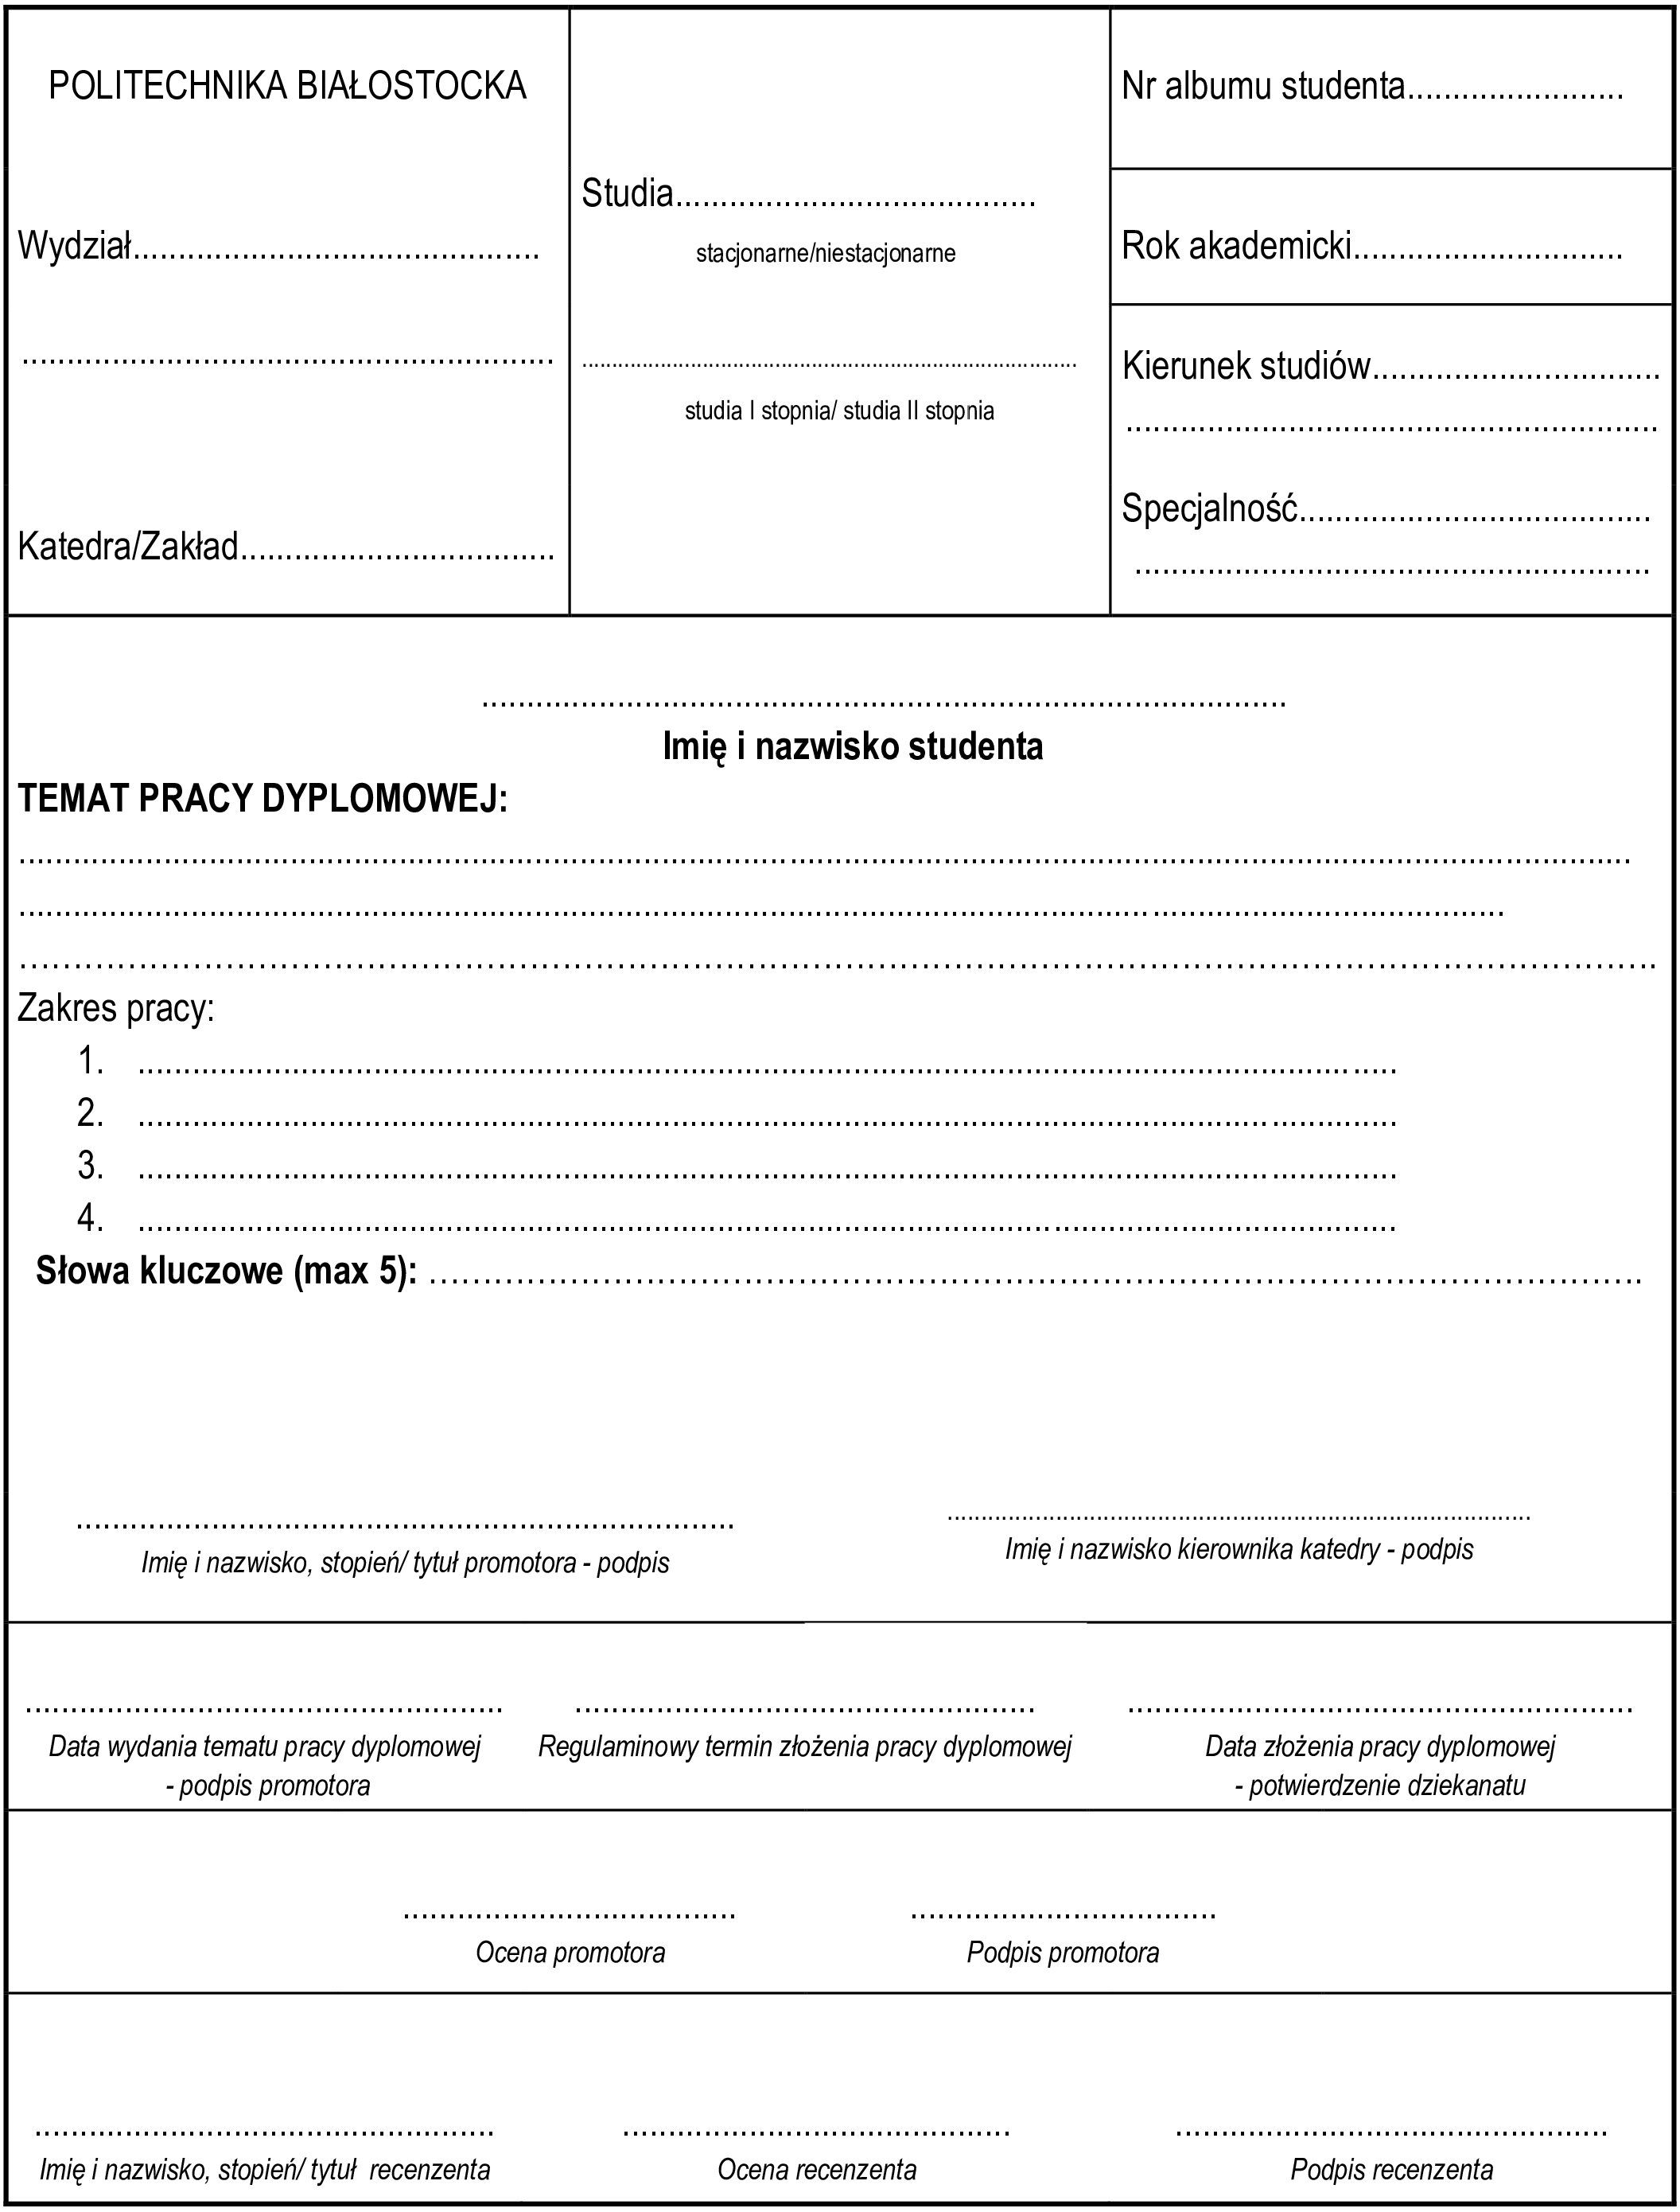
\includegraphics[width=\linewidth]{img/kartaDyplomowa.png}
\end{center}
\restoregeometry

%THESIS SUMMARY
\textbf{Thesis topic}: \textbf Comparison of performance and methods of implementing databases in iOS\par
\textbf{SUMMARY}: The purpose of this study was to compare the performance of selected databases and how to implement them in iOS. Each database has been implemented separately in a standard way for a given database The study compared the different types are typically relational databases and NoSQL (column-oriented), so it was an important aspect of ensuring adequate test environments, which can ensure the correctness of the results obtained regardless of differences in architecture. The work also presents a comparison of the methods of implementing the tested databases.

%STATEMENT
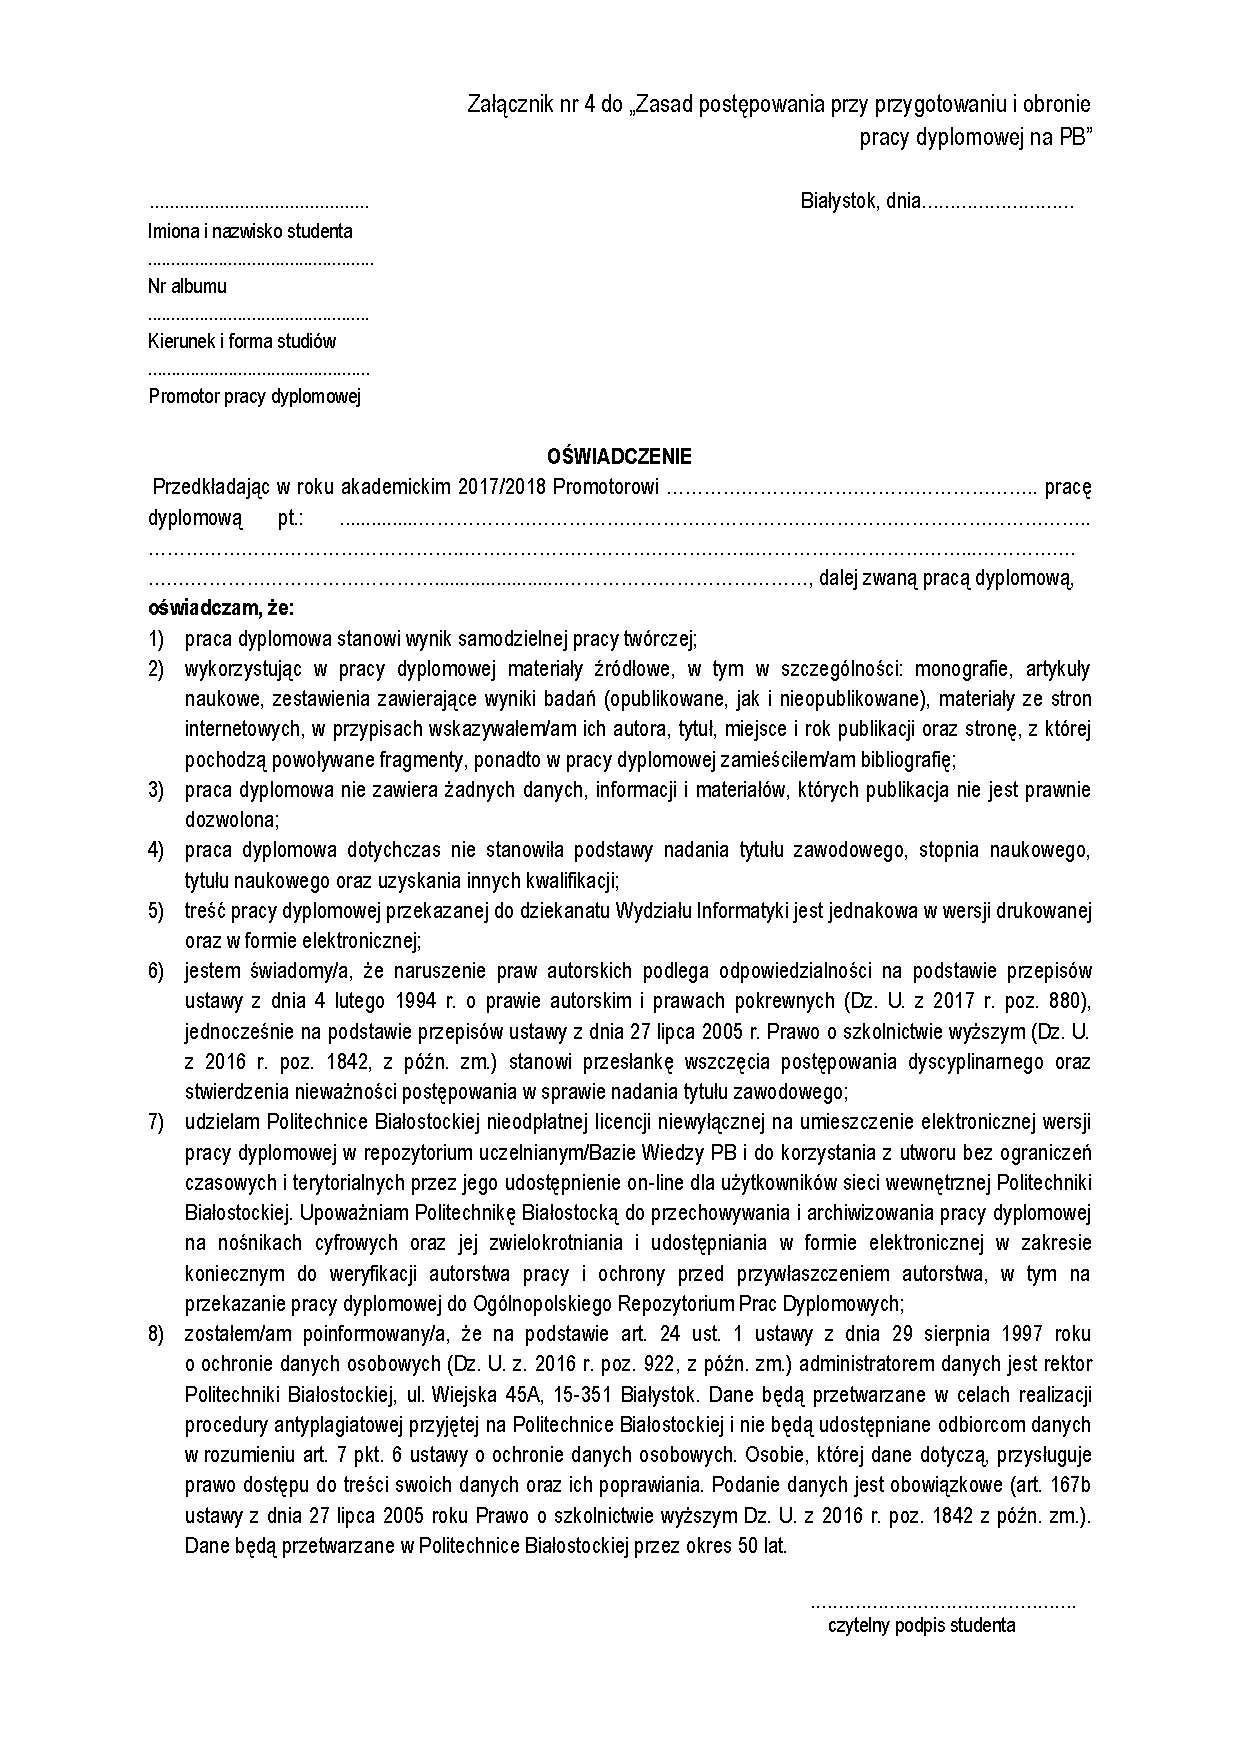
\includepdf[pages=1]{img/oswiadczenie-2017.pdf}
%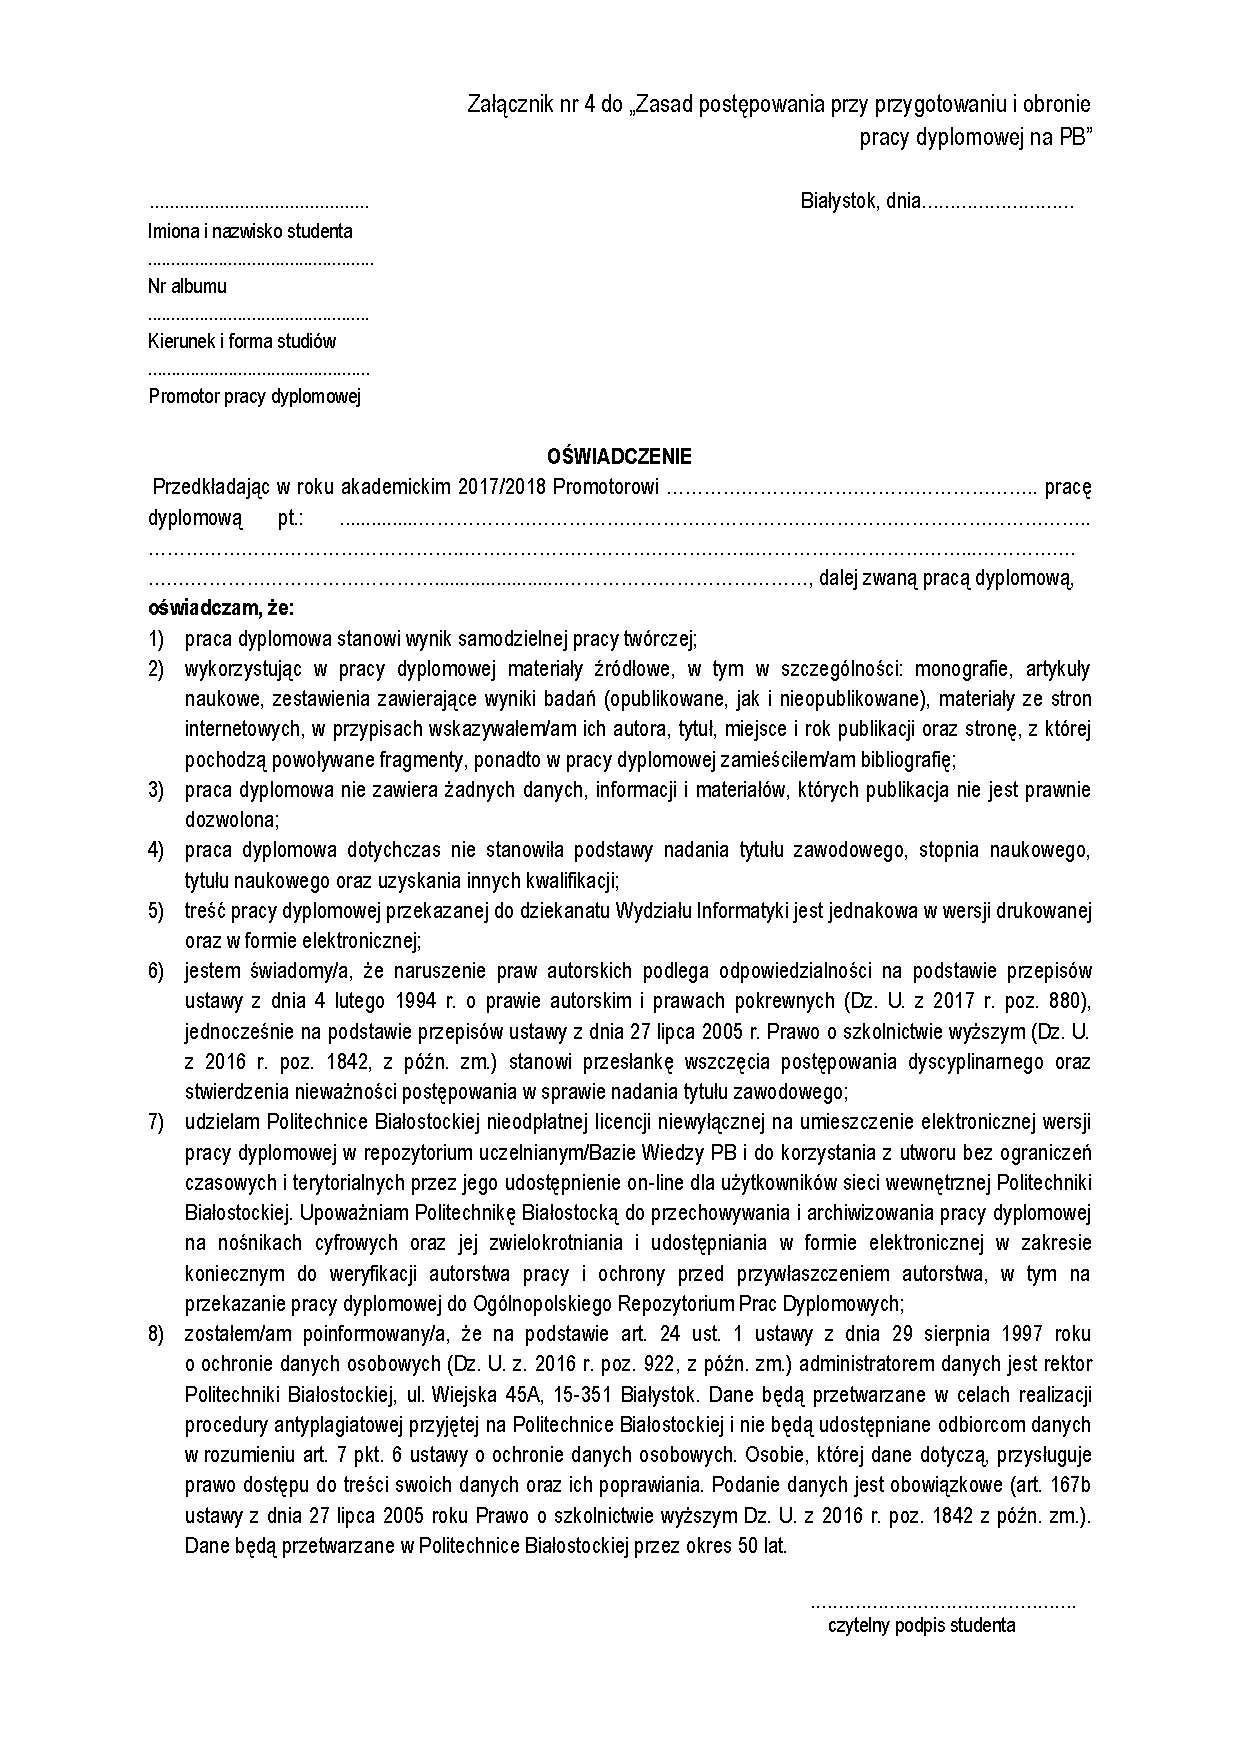
\includepdf[pages=-,pagecommand={},width=\textwidth]{img/oswiadczenie-2017.pdf}

%TABLE OF CONTENTS (spis treści)
\tableofcontents

%-----------------YOUR CONTENT STARTS HERE-------------------
\section{Wstęp}

 W~dzisiejszych czasach, kiedy dostęp do urządzeń mobilnych stał się powszechny, a~większość tych urządzeń dorównuje swoimi parametrami tabletom czy też nawet laptopom aplikacje mobilne stały się bardzo popularne. Wraz ze wzrostem popularności aplikacji pisanych na smatphony wymagania stawiane przed tymi programami znacząco wzrosły. Od najprostszych aplikacji wymaga się najczęściej spotykanych funkcjonalności stron internetowych lub aplikacji komputerowych takich jak połączenie z~internetem, uwierzytelnianie użytkownika, synchronizacji i~zapisu danych. \nocite{Swift-doc} \nocite{Realm-doc} \nocite{FMDB-doc} \nocite{CoreData-doc} \nocite{PorownanieRealm} \nocite{Mockaroo} \nocite{PorownanieDrDobbs} \nocite{SQLite-book} \nocite{CoreDataBook} \nocite{Art2Key} \nocite{Art3Key} \nocite{Art4Key}
\par
Obecnie praktycznie każda z~aplikacji zawiera w~sobie bazę danych. Synchronizowaną z~serwerem, przechowującą znaczące ilości danych odpowiadających za poprawne działanie programu, a~także często zapewniającą prace aplikacji bez połączenia z~internetem. Ważne jest więc aby zastosowana baza danych zapewniała satysfakcjonującą prędkości dostępu do danych i~nie narażała użytkownika na opóźnienia związane z~pozyskaniem danych. Istotną kwestią z~punktu widzenia programisty - osoby tworzącej aplikację jest łatwość implementacji wydajnej bazy danych. Łatwość implementacji przekłada się w~późniejszych etapach życia oprogramowania na szybsze i~prostsze dodawanie nowych elementów, relacji czy tablic w~zastosowanej bazie, dzięki czemu oszczędzany jest cenny czas przeznaczony na proces wytwarzania programu. \par

Niniejsza praca ma na celu przedstawienie obecnie dostępnych baz danych dla systemu iOS, pokazanie i~porównanie  sposobów ich implementacji oraz porównanie ich szybkości. Na potrzeby pracy stworzono aplikacje będącą środowiskiem testowym wybranych baz danych. 
	
\subsection{Cel pracy}

Celem niniejszej pracy było porównanie wydajności wybranych baz danych oraz sposobów ich implementacji w~systemie iOS. Każda z~baz została zaimplementowana oddzielnie w~standardowy dla danej bazy sposób. W~pracy porównane zostały różne typy baz danych typowo relacyjnych jak i~NoSQL (column-oriented), ważnym aspektem było więc zapewnienie odpowiednich środowisk testowych, które mogły zapewnić poprawność otrzymanych wyników niezależnie od różnic w~architekturze. Praca przedstawia również porównanie sposobów implementacji testowanych baz danych.\par

Zakres pracy obejmuje następujące zagadnienia: 

\begin{itemize}
	\item Wykonanie zbiorczego przeglądu literatury w~tematyce
	\item Opis dostępnych baz danych w~systemie iOS (Core data, SQLite, Realm, UserDefaults, FMDB)
	\item Stworzenie narzędzia do porównania wydajności baz danych oraz metod testowych.
	\item Przygotowanie struktury testów porównawczych i~środowisk testowych
	\item Zebranie wyników testów dla wybranych operacji oraz analiza wyników.
	\item Opis wniosków na podstawie zebranych danych badawczych.
\end{itemize}

\subsection{Struktura pracy}

Praca składa się z~siedmiu rozdziałów:

\begin{itemize}
	\item  Opis wybranych baz danych - w~rozdziale przedstawione zostały opisy wybranych baz danych dla systemu iOS: Core Data, Realm, FMDB oraz User Defaults. 
	\item Dostępne porównania baz danych - w~rozdziale zostały przedstawione dostępne porównania szybkości niektórych baz danych.
	\item Narzędzie do porównywania wydajności i~model bazy - w~rozdziale została przedstawiona aplikacja umożliwiająca przeprowadzenie testów wybranych baz danych. Pokazana zostanie struktura testowej bazy danych oraz opisane zostały przeprowadzane testy.
	\item Opis przeprowadzonych testów - w~rozdziale zostały opisane testy przeprowadzone w~ramach pracy. Przedstawiono kroki potrzebne do otrzymania poprawnych wyników w~zależności od typu testu oraz pokazano w~jaki sposób został mierzony czas uzyskania rezultatu każdej operacji. 
		\item Różnice implementacji baz danych -
 w~rozdziale zostały pokazane różnice i~podobieństwa w~implementacji poszczególnych rozwiązań bazodanowych. Przedstawiono fragmenty kodów wykonujące te same operacje przy użyciu różnych baz danych. Opisany też został stopień skomplikowania każdej z~operacji.
	\item Analiza - w~rozdziale zostały przedstawione wyniki przeprowadzonych testów. Każdy z~rezultatów testów został zanalizowany i~opisany.
\item Podsumowanie - zawarte są w~nim wnioski i~analiza rezultatów pracy.
\end{itemize}


\section{Opis wybranych baz danych}

 W~tym rozdziale przedstawione zostały opisy wybranych baz danych dla systemu iOS: Core Data, Realm, FMDB oraz User Defaults. W~systemie iOS istnieje wiele rozwiązań umożliwiających wdrożenie bazy danych w~aplikacji, przedstawione tutaj przykłady są jednymi z~najczęściej stosowanych przez programistów bazami danych w~aplikacjach iOS.

\subsection{SQLite}
SQLite jest wewnątrz procesową biblioteką dostępną w~systemie iOS. Kod opisywanej bazy jest dostępny publicznie, można go używać w~dowolnym celu komercyjnym lub prywatnym bez żadnych opłat. Sprawia to, że baza ta jest jednym z~najczęściej wybieranych przez programistów rozwiązań do przechowywania danych w~aplikacjach. Wybór tej biblioteki jest też kierowany tym, iż projekt istnieje już od 2000 roku, a~jego twórcy deklarują wsparcie aż do 2050 roku\cite{SQLite-doc}.\par

SQLite jest ,,lżejszą" wersją SQL więc korzystanie z~funkcji biblioteki zostało znacząco uproszczone. Baza ta nie posiada wydzielonych procesów serwerowych, dane zapisuje i~odczytuje ze zwykłych plików dyskowych. Kompletna baza danych programu zawierająca wszystkie tabele, relacje i~tym podobne komponenty zapewniające poprawne działanie bazy, przechowywane są w~jednym pliku na dysku. Dzięki przechowywaniu wszystkich tych informacji w~jednym pliku informacje te mogą być kopiowane w~stanie nienaruszonym pomiędzy programami.\par

System iOS zapewnia wbudowaną obsługę baz SQLite, nie istnieje więc potrzeba dodawania do projektu dodatkowych bibliotek. Cała komunikacja z~biblioteką jest natywna i~wymaga jedynie zaimportowania SQLite3\cite{SQLite-doc}. 
SQLite jest bazą relacyjną i~zapewnia dodawanie relacji pomiędzy tabelami takich jak: 

\begin{itemize}
  \item N:M – wiele do wielu
  \item 1:N – jeden do wielu
  \item 1:1 – jeden do jednego 
\end{itemize}

Zapewniona została też obsługa danych takich jak: 

\begin{itemize}
	\item NULL - wartość pusta
	\item INTEGER - wartość całkowita ze znakiem, przechowywana w~1, 2, 3, 4, 6 lub 8 bajtach w~zależności od wielkości wartości
	\item REAL - wartość zmiennoprzecinkowa, przechowywana jako 8-bajtowa liczba zmiennoprzecinkowa IEEE
	\item TEXT - wartością jest ciąg znaków przechowywany przy użyciu kodowania bazy danych (UTF-8, UTF-16)
	\item BLOB - wartość przeznaczona do przechowywania wielkich plików w~formie bajtowej takich jak obrazy, muzyka itp. 
\end{itemize}

SQLite nie zapewnia wsparcia dla przechowywania obiektów zawierających datę. W~celu zapisania daty w~tablicy należy używać wartości tekstowych lub liczbowych, a~następnie zapewnić ich odpowiednie odczytanie i~konwersje do odpowiednich obiektów języka, w~którym przebiega implementacja programu. 

\subsection{Core Data}

Core Data jest dedykowanym rozwiązaniem Apple umożliwiającym zaimplementowanie bazy danych w~aplikacjach iOS i~MacOS. Została wprowadzona od wersji iOS 3.0 w~2009 roku. Znacznie szybciej istniała możliwość używania tej bazy danych w~MacOS. Pierwszą wersją systemu dającego możliwość użyawnia Core Data był MacOS Tiger, który ukazał się w~2005 roku\cite{CoreData-doc}.\par

Mimo że Core Data służy do przechowywania danych sama w~sobie nie jest bazą danych a~framework'iem, który zarządza diagramem obiektów aplikacji. Diagram obiektów jest to zbiór obiektów powiązanych ze sobą relacjami. Core Data zajmuje się zarządzaniem cyklem życia obiektów w~diagramie obiektów na dysku, a~także oferuje interfejs do przeszukiwania obiektów, którymi zarządza. Core Data daje także możliwość sprawdzania poprawności danych wejściowych, modelowania modeli danych czy też śledzenia zmian. \par

Core Data jako rozwiązanie implementacji bazy danych korzysta z~SQLite, przechowuje za jego pomocą wszystkie obiekty na dysku. Rozszerza jednak oferowane funkcjonalności SQLite o~obsługę bazy w~kilku wątkach, tworzenia tymczasowych obiektów (kiedy nie jesteśmy pewni, czy one zostaną zapisane na dysk), automatycznie nasłuchiwanie na zmiany w~bazie danych między innymi, jeśli wyświetlamy dane użytkownika na ekranie, a~dane w~bazie danych się zmienią (za sprawą na przykład drugiego wątku pracującego z~zewnętrznym serwerem API), to dostaniemy odpowiednie powiadomienie. Core Data zapewnia łatwą integrację z~kontrolkami interfejsu użytkownika takimi jak UITableView (kontrolka odpowiedzialna za wyświetlanie tabel/list) między innymi zapewniając automatyczne tworzenie indeksów i~sekcji.\par

Core Data jest zorganizowana w~dużą hierarchię klas, lecz używane są najczęściej podstawowe obiekty takie jak: 

\begin{itemize}
	\item NSManagedObject - Klasa reprezentująca jeden wiersz tabeli, zapewniajacy dostęp do danych przechowywanych w~wierszu.
	\item NSManagedObjectContext - Główny kontekst bazy, wykonuje operacje na bazie. Pozwala na zapis aktualnego stanu bazy danych.
	\item NSManagedObjectModel	- Klasa reprezentujący model tablicy. 
	\item NSFetchRequest - Klasa pozwalająca utworzyć zapytanie mające na celu przeprowadzenie operacji na danych.
	\item NSPersistentStoreCoordinator - Klasa odpowiedzialna za operacje na pliku, który przechowuje dane bazy. Za pomocą tej klasy możliwe jest całkowite jest usunięcie. 
	\item NSPredicate - Klasa za pomocą, której tworzymu zapytanie do bazy danych, używana jest jako parametr metody klasy NSFetchRequest.
\end{itemize}

Tak samo, jak poprzednio opisywana baza danych Core Data pozwala na tworzenie wszystkich możliwych relacji pomiędzy tabelami. Framework zapewnia też możliwość przechowywania w~tabeli wielu typów danych takich jak: 

\begin{itemize}
	\item String - łańcuch znaków
	\item Int - liczba całkowita
	\item Float - liczba zmiennoprzecinkowa
	\item Double  - liczba zmiennoprzecinkowa
	\item Boolean - wartość boolowaska prawda/fałsz 
	\item Date - obiekt przechowujący date
	\item Binary Data - dane w~formacie binarnym 
	\item URI - adresy zasobów
	\item Transformable - wartość do przechowywana niestandardowych danych 
\end{itemize}

Jedną z~ważnych cech tej bazy danych jest możliwość graficznego definiowania schematu bazy, pełne wsparcie zapewnia środowisko programistyczne XCode. Na rysunku  poniżej został przedstawiony edytor bazy danych. \par

\begin{figure}[h]
	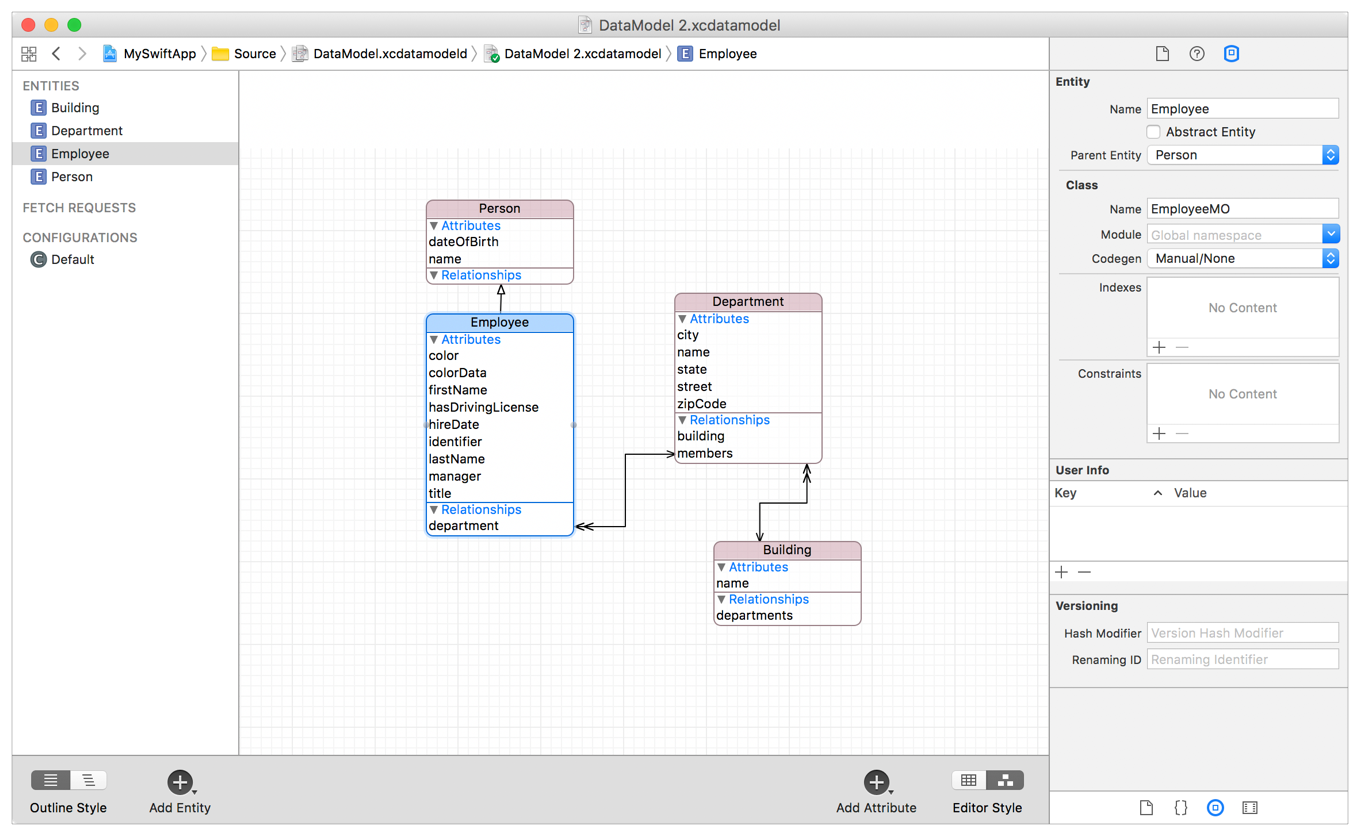
\includegraphics[width=\linewidth]{img/Entity_Inheritence_2_2x.png}
	\caption{Edytor Core Data w~XCode}
	\label{fig: CoreDataEdytor}
\end{figure}

Dodatkowo XCode pozwala generować klasy dla obiektów stworzonych za pomocą edytora, które wykorzystywane są później do tworzenia obiektów przed zapisem do bazy. Istnieją też inne narzędzia, które umożliwiają wygenerowanie klas dla stworzonego diagramu. Jednym z~najpopularniejszym jest Mogenerator. Zapewnia on wsparcie dla języka Swift i~Objective-C.

\newpage
\subsection{FMDB}

FMDB jest biblioteką opakowującą SQLite. Można więc stwierdzić, że FMDB i~SQLite służą temu samemu celowi - umożliwiają efektywne zarządzanie danymi aplikacji. Mimo pokrewieństwa bibliotek sposoby ich używania znacząco się od siebie różnią. FMBD oferuje interfejs wyższego poziomu, ukrywając wszystkie szczegóły SQL takie jak połączenie i~komunikacja z~bazą, ale dalej oferuje dokładną obsługę danych. \par 
FMDB zapewnia funkcje SQLite, więc podczas implementacji nie trzeba zajmować się połączeniami, a~także pisaniem i~odczytywaniem danych do i~z bazy. Biblioteka ta jest dobrym rozwiązaniem dla programistów, którzy chcą wykorzystać swoją wiedzę SQL i~pisać własne zapytania, ale bez potrzeby pisania własnego menadżera SQLite. FMDB działa w~dwóch językach: Swift i~Objective-C oraz bardzo szybko integruję się z~projektem iOS. Jej twórcy zapewniają, że jest ona zaimplementowana tak, aby zapewnić najwyższą wydajność SQLite, lepszą od prostych implementacji menadżerów dla SQLite. \par

Biblioteka jest bardzo prosta w~użyciu. Możemy w~niej wyróżnić trzy główne klasy: 

\begin{itemize}
	\item  FMDatabase - Reprezentuje pojedynczy obiekt bazy danych. Używana jest do wykonywania instrukcji SQL. 
	\item FMResultSet - Klasa przetrzymująca rezultaty zapytań SQL wykonanych na bazie danych.
	\item FMDatabaseQueue - Klasa, która jest używana podczas wykonywania kwerend i~aktualizacji danych w~bazie przy użyciu wielu wątków.
\end{itemize}

Jako że FMBD oferuje interfejs wyższego poziomu do SQLite dodana została obsługa typów danych takich jak: 

\begin{itemize}
	\item Bool -  wartość boolowaska prawda/fałsz 
	\item Date - obiekt przechowujący date
\end{itemize}

Obsługa tych dwóch typów danych wymagała w~SQLite dodatkowych operacji. W~przypadku wartości prawda/fałsz należało zapisywać w~tabeli zero lub jeden i~odpowiednio konwertować wartości liczbowe do wartości Bool. Sytuacja podczas zapisu daty w~SQLite wygląda podobnie, należy najpierw wartość daty skonwertować do wartości tekstowej, a~podczas odczytu danych wartość tekstową skonwertować do obiektu przechowującego datę. FMBD w~znaczącym stopniu ułatwia obsługę tak często używanych w~bazach danych wartości. Dodatkowo warto wspomnieć, iż FMDB będąc biblioteką opakowującą SQLite daje możliwość korzystania z~dokumentacji SQLite, która jest bardzo dokładna i~ciągle rozwijana. Trudno więc zaprzeczyć, że biblioteka ta stanowi dobre rozwiązanie zastępujące standardowy SQLite. 

\subsection{Realm}

Realm różni się od poprzednio opisywanych baz SQL. Biblioteka ta jest obiektową bazą danych NoSQL. Przechowuje dane w~postaci obiektów. Realm jest rozwiązaniem open-source, więc jest w~pełni darmową bazą danych, dedykowaną do aplikacji mobilnych. Dodatkowo jest dostępna na systemy Android i~iOS, co znacząco ułatwia prace nad aplikacjami dostępnymi nie tylko na jedną platformę. Współpracuje z~projektami pisanymi w: Swift, Objective-C, Java, React Native, Xamarin i~innymi. Biblioteka ujrzała światło dzienne w~2016 roku, a~pierwsza stabilna wersja wydana została w~styczniu 2017 roku. Jedną z~wyróżniających ją funkcji jest możliwość dwukierunkowej synchronizacji pomiędzy bazą serwera, a~bazą aplikacji.\par 

Realm swoją popularność zyskał poprzez szybkość, łatwość integracji z~projektem oraz łatwością posługiwania się nim. Od bibliotek opakowujących SQLite oraz całego framework-u Core Data odróżnia go to, że większość typowych funkcji, takich jak odpytywanie bazy danych składa się, z~pojedynczych linii kodu. Dzięki temu, używając biblioteki Realm, uzyskuje się bardziej zwięzły kod i~poprawia się jego czytelność. Podczas używania Realm niepotrzebna jest dobra znajomość SQL do zarządzania bazą i~tworzenia zapytań. Nie wymagana jest też dobra znajomość Core Data, która jest zaawansowanym narzędziem i~nie wiele osób ma umiejętności, pozwalające wydajnie zarządzać tą bazą danych. W~Realm dane są przechowywane jako obiekty, dzięki czemu przy odczytywaniu czy zapisywaniu danych w~bazie nie ma potrzeby stosowania żadnej biblioteki ORM (Object Relation Mapping), pozwalającej na konwersje danych pomiędzy obiektem programu, a~rekordem tabeli. Dzięki temu nie występują problemy z~wydajnością dodatkowych bibliotek ORM. Interfejs biblioteki ogranicza się do trzech klas: 

\begin{itemize}
	\item Realm -  Główna klasa, pozwalająca na dostęp do bazy i~wykonywanie operacji zapisu/odczytu.
	\item Object - Klasa reprezentująca model danych bazy.
	\item Result - Obiekt reprezentujący listę dane odczytane z~bazy przy użyciu zapytania.
\end{itemize}
 \par

Realm tak jak Core Data czy FMDB zapewnia wsparcie dla wszystkich typów danych. Na uwagę zasługują tutaj relacje pomiędzy tabelami. Biblioteka jest obiektową bazą danych, nie ma więc w~niej tabel i~zwykłych relacji pomiędzy nimi. W~Realm relacje pomiędzy obiektami tworzone są za pomocą linkowana obiektów. Każdy link tworzy link zwrotny, jako relację odwrotną do dowolnego obiektu łączącego się z~bieżącym obiektem. Za pomocą Reaml Studio możliwe jest także stworzenie pliku bazy danych na podstawie dokumentu CSV.  \par 

Dodatkowo Realm dostarcza również narzędzie Realm Studio, widoczne na rysunku 2.2. Pozwala ono na łatwe zarządzanie bazą danych. Umożliwia otwieranie, przeglądanie i~edytowanie lokalnych plików Realm.  

\begin{figure}[h]
	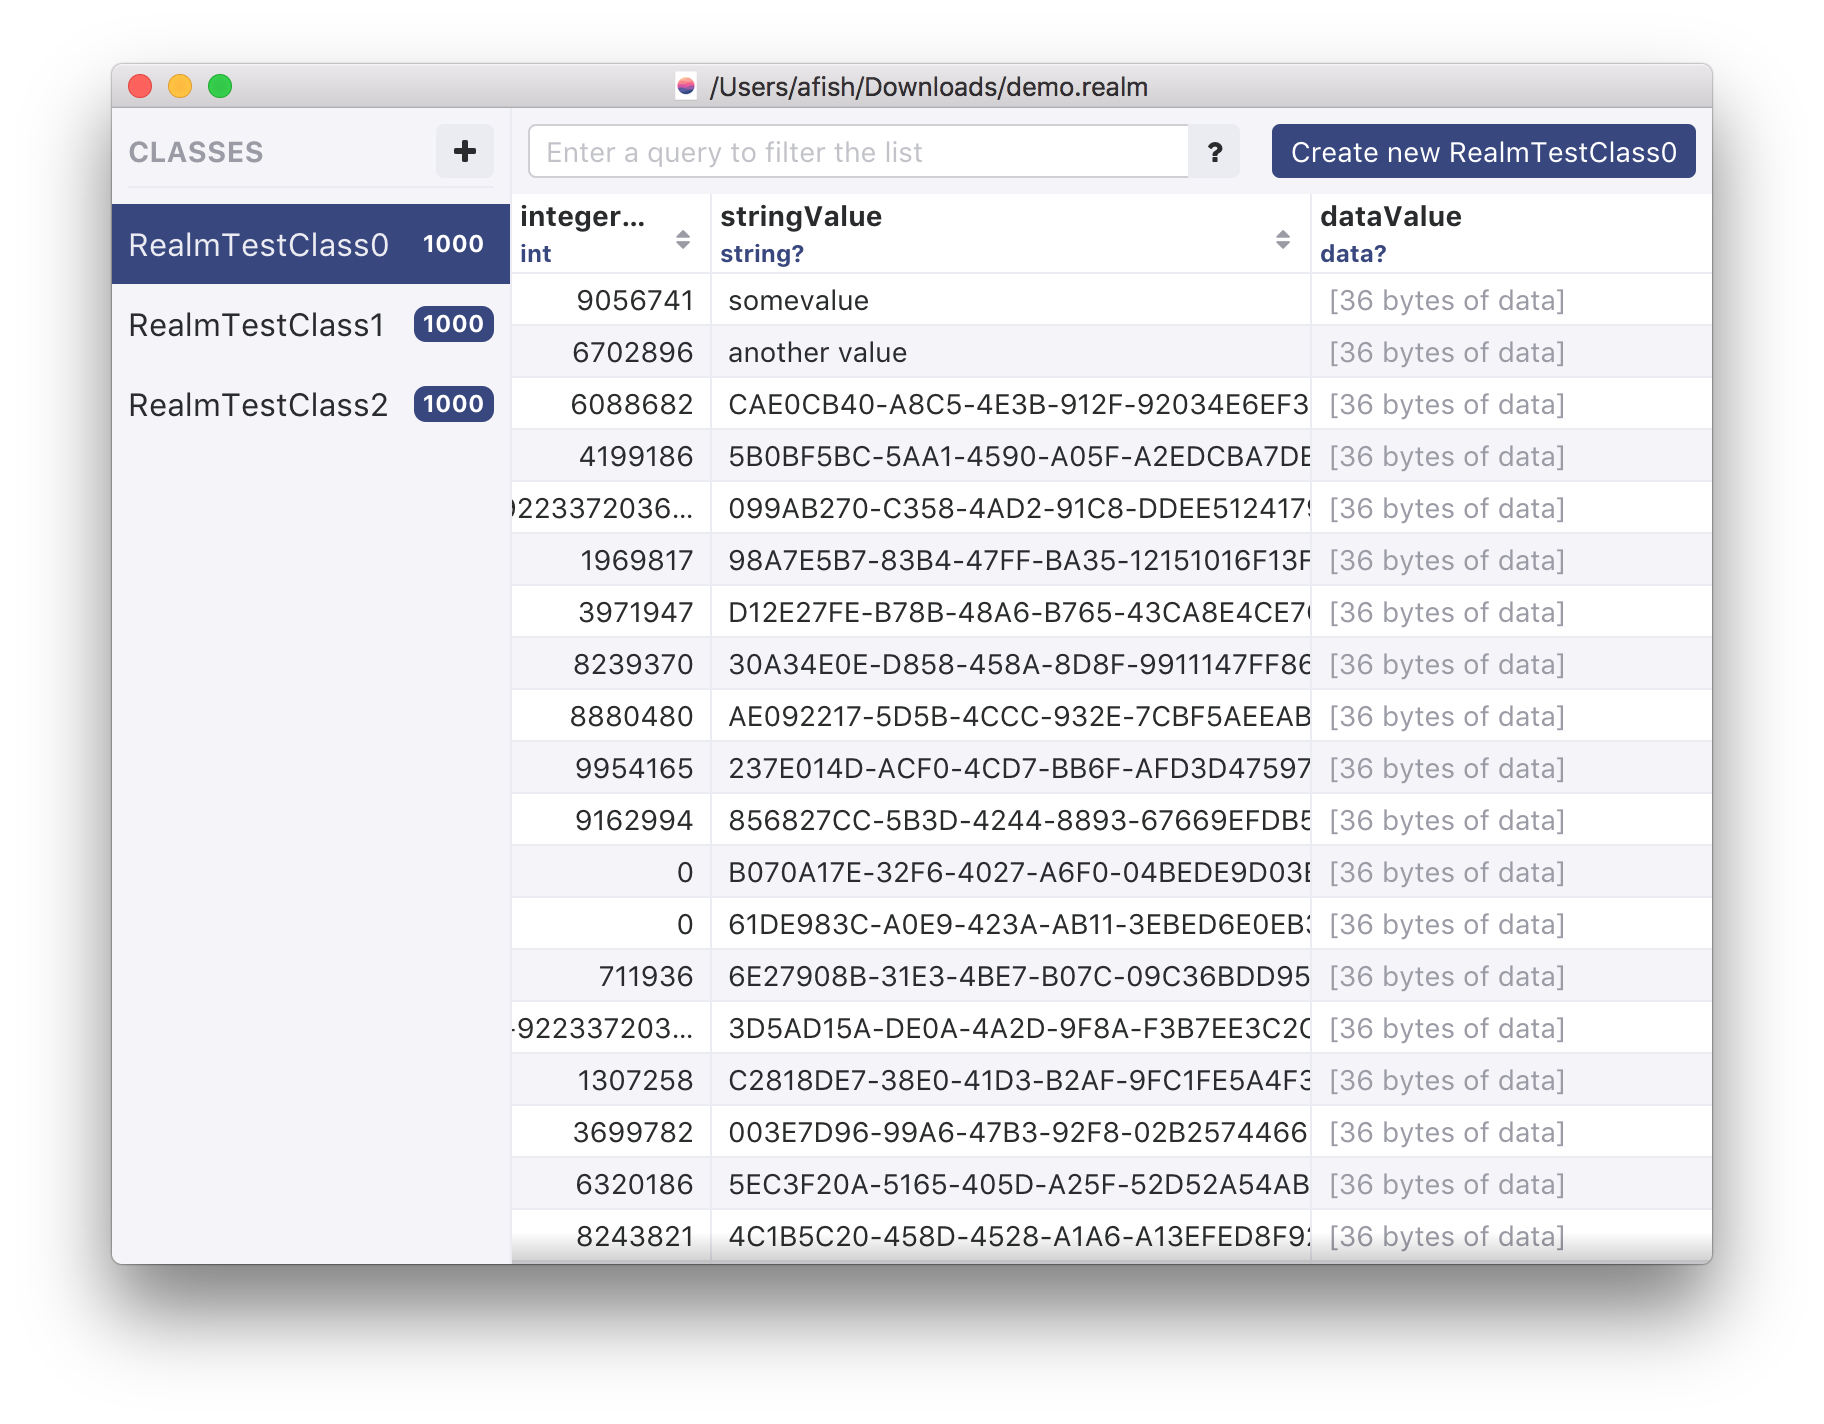
\includegraphics[width=\linewidth]{img/RealmStudio.png}
	\caption{Narzędzie Realm Studio}
	\label{fig: RealmStudio}
\end{figure}

\subsection{User Defaults}

Kolejnym z~rozwiązań pozwalającym zapisywać i~przechowywać dane w~systemi iOS jest User Defaults - domyślna baza użytkownika. Dane w~niej przechowywane są pary klucz - wartość. System, pomimo iż nie jest prawdziwą bazą danych, a~jedynie interfejsem, który pozwala na przechowywanie potrzebnych, niewielkich danych aplikacji, został wybrany w~tej pracy do porównania, ponieważ wielu programistów używa go zamiast innych rozwiązań bazodanowych. Rozwiązanie to jest szybkie w~implementacji i~pozwala zapisywać niestandardowe obiekty, jeżeli implementują protokół NSCoding i~zostaną skonwertowane do prostej formy Data. Więcej informacji na temat sposobu zapisu i~konwersji danych znajduję się w~rozdziale 6 . \par
  
User Defaults pozwala zapisywać wartości takie jak: Bool, Integer, Float, Double, String, Data, URL, Array, Dictionary. Zapis danych wykonuje się za pomocą funkcji set(:forKey:), a~odczyt value(forKey:). 

\section{Przegląd literatury - dostępne porównania baz danych}

 W~rozdziale zostały przedstawione dostępne porównania szybkości niektórych baz danych. Przytoczone porównania są w~pewnym stopniu punktem odniesienia do uzyskanych w~pracy wyników. W~każdym z~przypadków uzyskane wyniki są inne, testy były przeprowadzane na różnych danych. Różna była też ilość danych i~ich złożoność, a~także sposób implementacji bibliotek. 

\subsection{Core Data i~SQLite - porównanie wydajności}

Porównanie zaczerpnięte z~witryny internetowej http://www.drdobbs.com. Autor stworzył przykładową aplikację pozwalająca przeprowadzić operacje na głównych bazach danych iOS. Testy zostały przeprowadzone na iPhone 5s. \par

Do testów został użyty prosty zestaw danych, który jest widoczny na rysunku 3.1 znajdującym się poniżej. 

\begin{figure}[h]
	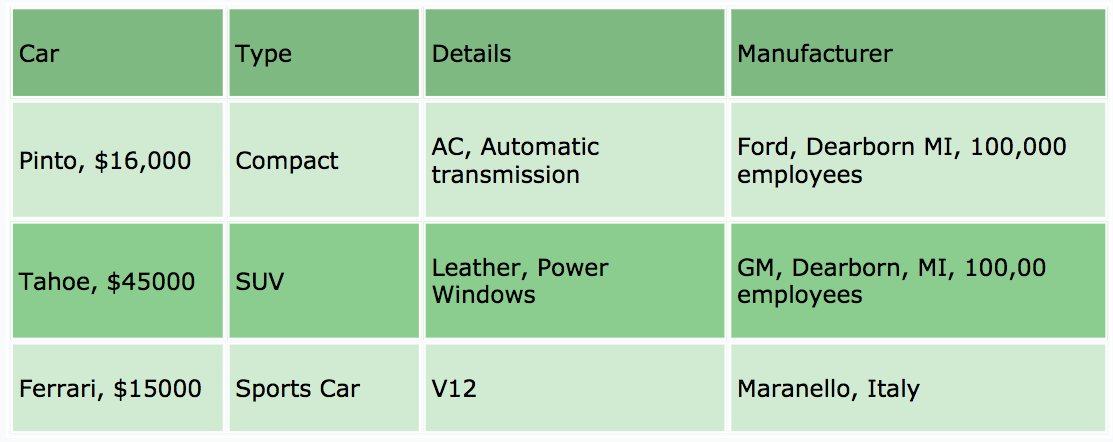
\includegraphics[width=\linewidth]{img/coredata_sql_test.png}
	\caption{Przykład danych użytych do porównania wydajności Core Data i~SQLite}
	\label{fig: CoreData_SQLite_test_data}
\end{figure}

%\begin{table}[]
%\begin{tabular}{|c|c|c|c|}
%\hline
%\rowcolor[HTML]{72B076} 
%Car              & Type       & Details                                                               & Manufacturer                                                                    \\ \hline
%\rowcolor[HTML]{CAE8CC} 
%Pinto, \$16,000  & Compact    & \begin{tabular}[c]{@{}c@{}}AC, \\ Automatic transmission\end{tabular} & \begin{tabular}[c]{@{}c@{}}Ford, Dearborn MI, 100,000 \\ employees\end{tabular} \\ \hline
%\rowcolor[HTML]{72B076} 
%Tahoe, \$45000   & SUV        & \begin{tabular}[c]{@{}c@{}}Leather, \\ Power Windows\end{tabular}     & \begin{tabular}[c]{@{}c@{}}GM, Dearborn, MI, 100,00 \\ employees\end{tabular}   \\ \hline
%\rowcolor[HTML]{CAE8CC} 
%Ferrari, \$15000 & Sports Car & V12                                                                   & Maranello, Italy                                                                \\ \hline
%\end{tabular}
%\end{table}

Autor przeprowadził testy pokazujące zajętość pamięci obiektu bazy na dysku urządzenia, testy użycia pamięci aplikacji używającej bazy oraz testy szybkości bazy podczas pobierania danych z~bazy. Poniższe rysunki 3.2, 3.3, 3.4 prezentują ich rezultaty.

\begin{figure}
\centering
	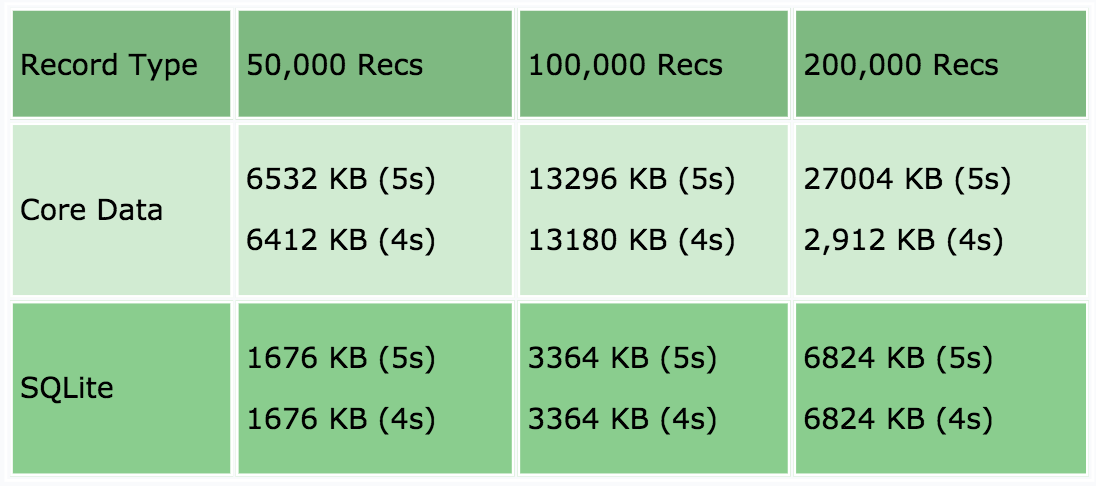
\includegraphics[width=13cm]{img/drdobbs_storage_test.png}
	\caption{Rezultat testów porównania Core Data i~SQLite - wielkość pliku bazy }
	\label{fig: CoreData_SQLite_storage_test}
\end{figure}

\begin{figure}
\centering
	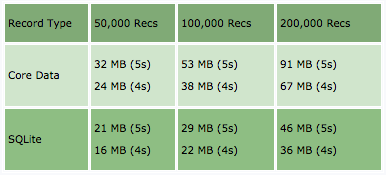
\includegraphics[width=13cm]{img/drdobbs_memory_test.png}
	\caption{Rezultat testów porównania Core Data i~SQLite - pamięć aplikacji}
	\label{fig: CoreData_SQLite_memory_test}
\end{figure}

\begin{figure}
\centering
	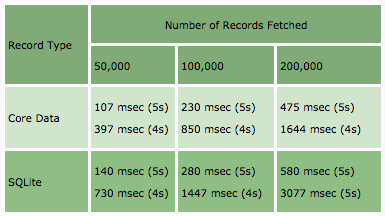
\includegraphics[width=13cm]{img/drdobbs_speed_test.png}
	\caption{Rezultat testów porównania Core Data i~SQLite - prędkość odczytu danych}
	\label{fig: CoreData_SQLite_speed_test}
\end{figure}
\clearpage

Wyniki wielkości pliku bazy pokazują, że plik bazy Core Data zajmuje około cztery razy więcej miejsca niż plik bazy SQLite. Na rysunku 3.3 widać, że Core Data zużywa też więcej pamięci operacyjnej podczas działania aplikacji. Autor tłumaczy, że wynika to ze sposobu, w~jaki działa Core Data. Tworzy ona w~pierwszej kolejności obiekty w~pamięci, a~dopiero później następuje zapis do bazy, przez co Core Data zużywa od 40\% do 100\% pamięci więcej niż SQLite. Rysunek 3.4 przedstawia czasy, w~jakich następuje kolejno odczyt 50 000, 100 000, 200 000 tysięcy rekordów z~baz. W~tym porównaniu znacząco dominuje Core Data. Na iPhone 4s osiąga dwukrotną szybkość odczytu danych. 

\subsection{Realm}

Wydawca Realm udostępnia na swojej stronie porównanie swojego rozwiązania z~bazami takimi jak: SQLite, FMDB, Core Data, Couchbase Lite, YapDatabase. W~testach zostały porównane prędkości zapisu danych, wykonania czasu zapytania oraz zliczenia rekordów. Poniższe rysunki pokazują ich wyniki. \par

\begin{figure}[h]
\centering
	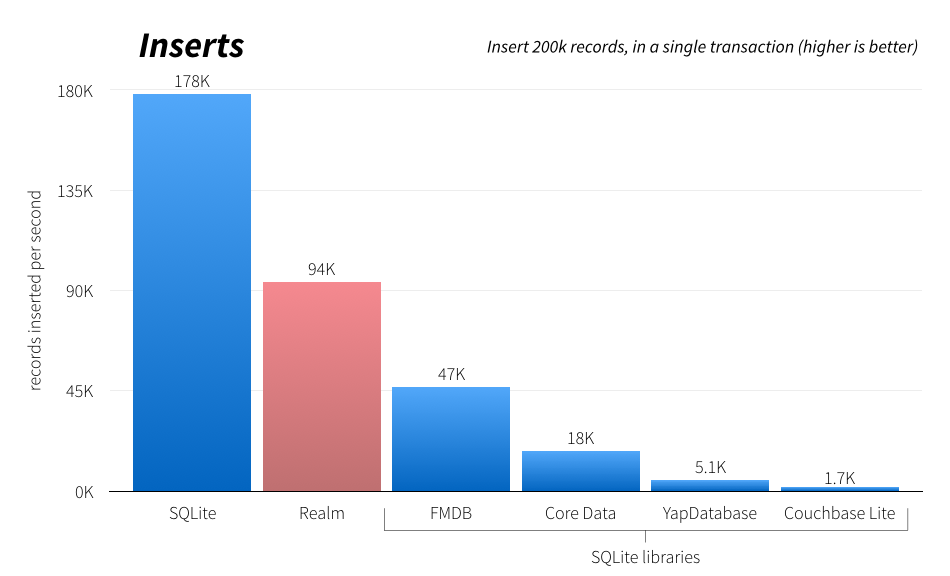
\includegraphics[width=\linewidth]{img/realm_insert_test.png}
	\caption{Rezultat testów Realm - zapis danych do bazy}
	\label{fig: realm_insert_test}
\end{figure}

\begin{figure}
\centering
	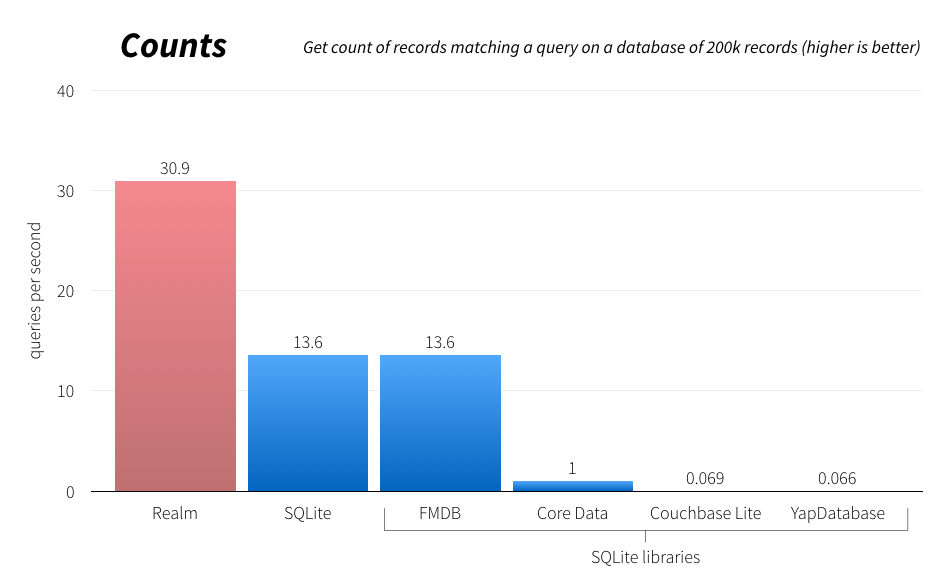
\includegraphics[width=\linewidth]{img/realm_count_test.png}
	\caption{Rezultat testów Realm - zliczanie rekordów}
	\label{fig: realm_count_test}
\end{figure}

\begin{figure}
\centering
	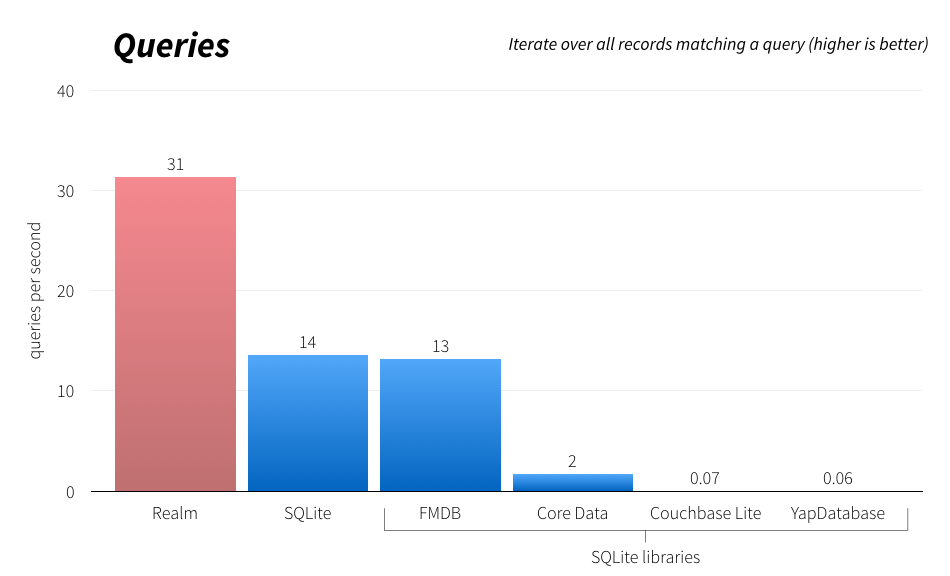
\includegraphics[width=\linewidth]{img/realm_query_test.png}
	\caption{Rezultat testów Realm - odczyt danych}
	\label{fig: realm_query_test}
\end{figure}
\clearpage

Realm w~opisach zapewnia, że ich produkt posiada doskonałą wydajność. Szybszą nawet w~niektórych przypadkach od SQLite. Testy wydają się potwierdzać ich słowa. SQLite wypadł gorzej od Realm tylko w~jednym teście, które przedstawili. Okazał się on najszybszy przy zapisie danych do bazy, osiągając blisko dwukrotnie wyższy wynik od Realm wynoszący 178 000 zapisanych rekordów w~ciągu sekundy, rezultat widoczny jest na rysunku 3.5. Kolejne testy pokazują dominacje Realm. W~teście zliczania rekordów SQLite i~FMDB uzyskują taki sam wynik - 13.6 operacji na sekundę zaś Realm wykonuje aż 30.9 operacji, co jest wynikiem ponad dwukrotnie wyższym. W~przypadku odczytu danych Realm też jest najszybszy. Osiąga wynik 31 operacji na sekundę a~SQLite i~FMDB jedynie 13-14 operacji. Wynik kolejny raz jest ponad dwukrotnie lepszy. \par 
Wynik testów są bardzo imponujące i~dowodzą, że Realm jest jedną z~najszybszych baz danych. Autorzy testów niestety nie pokazują sposobu testowania baz ani nie ujawniają, na danych jakiego typu odbyły się testy.

\section{Narzędzie do porównywania wydajności i model bazy }

W rozdziale zostanie przedstawiona aplikacja umożliwiająca przeprowadzenie testów wybranych baz danych. Pokazana zostanie struktura testowej bazy danych oraz opisane zostaną przeprowadzane testy.

\subsection{Aplikacja}

W celu przeprowadzenia testów wybranych baz danych stworzona została aplikacja umożliwiająca przetestowanie szybkości baz danych w systemie iOS. Na rysunku 4.1 znajdującym się poniżej pokazany został pierwszy ekran aplikacji umożliwiający wybranie baz danych do testów. 

\begin{figure}[h]
\centering
	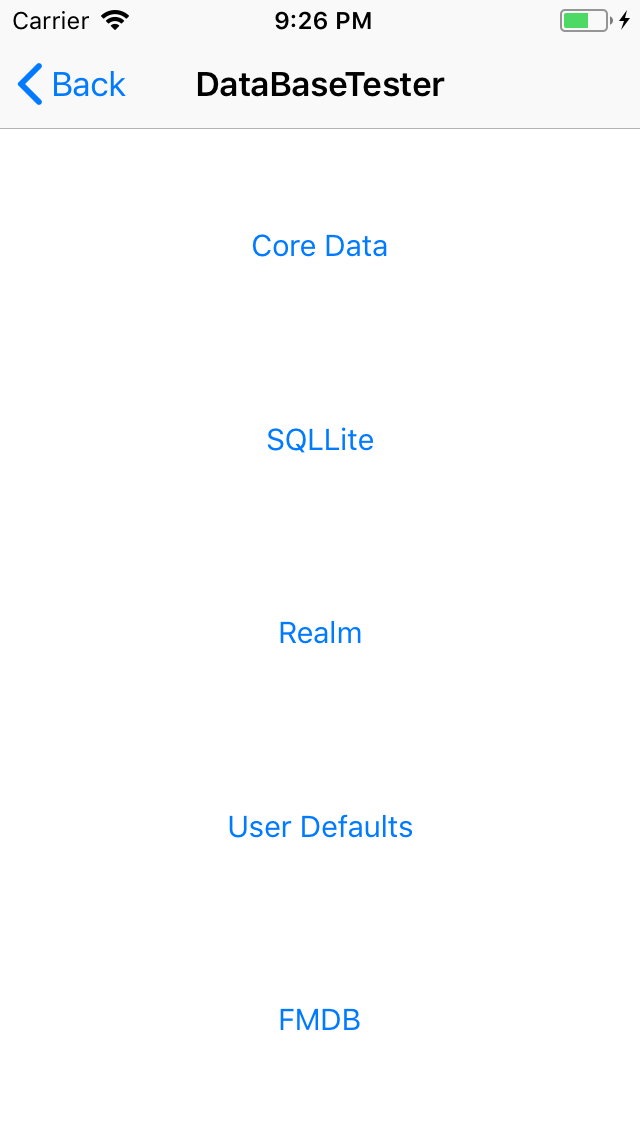
\includegraphics[width=6cm]{img/application/app-first-view.png}
	\caption{Ekran wyboru bazy danych do testów}
	\label{fig: first_app_view}
\end{figure}

Po wyborze bazy danych użytkownik zostaje przeniesiony do kolejnego ekranu aplikacji w którym należy wybrać jeden z dostępnych testów. Ekran widoczny jest na rysunku 4.2 znajdującym się poniżej.

\begin{figure}[h]
\centering
	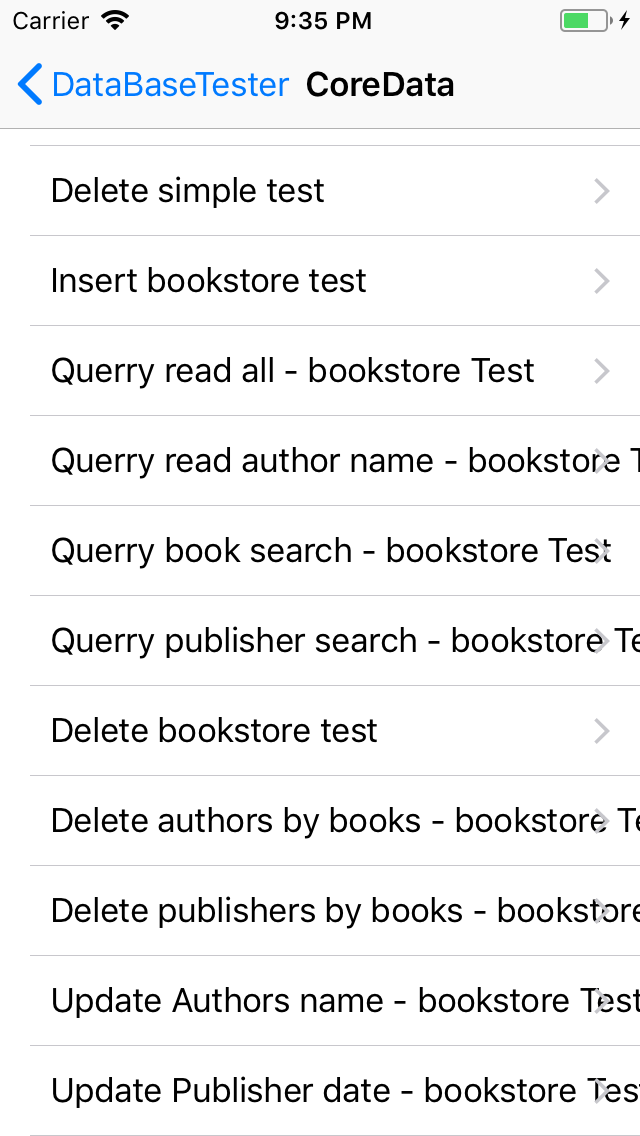
\includegraphics[width=6cm]{img/application/app-second-view.png}
	\caption{Ekran wyboru testu bazy danych}
	\label{fig: second_app_view}
\end{figure}

\newpage

Po wyborze jednego z testów następuje przejście do kolejnego ekranu widocznego na rysunku 4.3. Jest to ekran wyboru parametrów testu takich jak wielkość zestawu danych testowych i ilości powtórzeń testu. 

\begin{figure}[h]
\centering
	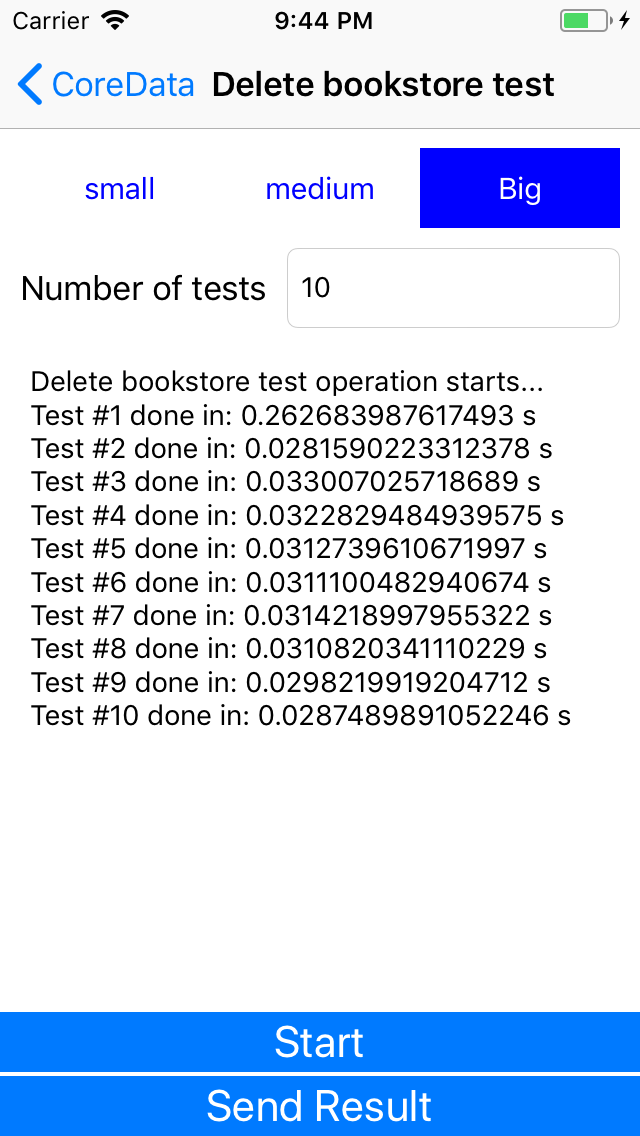
\includegraphics[width=6cm]{img/application/app_third-view.png}
	\caption{Ekran wykonywania testu}
	\label{fig: third_app_view}
\end{figure}

\newpage

Na ekranie znajduje się przycisk "Start" który uruchamia test. Podczas wykonywania testu na ekranie wypisywane są czasy w których zakończone zostają pojedyncze iteracje. Kiedy test dobiegnie końca za pomocą przycisku "Send Result" możliwa jest generacja pliku CSV zawierającego wszystkie uzyskane wyniki takie jak czasy pojedynczych operacji, użycie pamięci operacyjnej aplikacji podczas trwania testu czy też użycie procesora podczas każdej z przeprowadzanych operacji. 

\subsection{Schemat bazy danych}

Do przeprowadzenia testów zaprojektowany został prosty schemat bazy danych. Widoczny jest na rysunku 4.4. Zawiera on następujące tablice: Autor, Książka, Wydawnictwo. Autor może mieć wiele książek zaś książka wielu autorów - użyta została tu relacja wiele do wielu. Wydawnictwo może wiele książek ale jedna książka może mieć tylko jedno wydawnictwo - zastosowana została relacja jeden do wielu. 

\begin{figure}[h]
\centering
	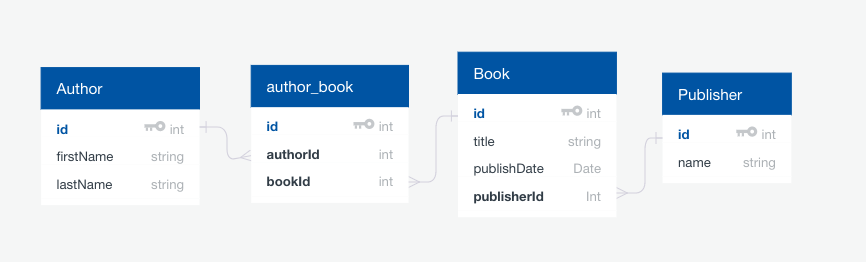
\includegraphics[width=\linewidth]{img/database/sql-scheme.png}
	\caption{Schemat basy danych SQL}
	\label{fig: sql_data_schame}
\end{figure}

Zaprojektowany schemat bazy umożliwia przetestowanie działania baz danych przy pracy na tabelach w których są różne typy relacji a także zapewnia możliwość testowania odczytu i zapisu daty. Data jest jednym z ważniejszych elementów w mobilnych bazach danych ponieważ niektóre rozwiązania bazodanowe nie zapewniają wsparcia dla tego formatu danych o czym była mowa podczas opisu wybranych baz danych. \par 

W pracy zostały użyte różne typy baz danych a mianowicie bazy NoSQL. Dla Realm i Core Data stworzony został schemat bazy widoczny na rysunku 4.5, nie posiadający tablicy pośredniej dla relacji wiele do wielu (Autor - Książka). Tablica ta jest zbędna dla tego typu baz danych ponieważ relacja wiele do wielu przechowywana jest za pomocą listy książek w tabeli autor i listy autorów w tablicy książka. 

\begin{figure}[h]
\centering
	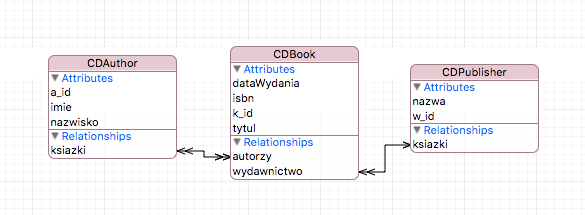
\includegraphics[width=\linewidth]{img/database/document-sheme.png}
	\caption{Schemat basy danych dla Realm i Core Data}
	\label{fig: nosql_data_scheme}
\end{figure}

Dla domyślnej bazy użytkownika - User Defaults struktura zapisywanych obiektów wygląda tak samo jak schemat dla baz NoSQL widoczny na rysunku 4.5. \par 

\section{Opis przeprowadzonych testów}

W rozdziale zostały opisane testy przeprowadzone w ramach pracy. Przedstawiono kroki potrzebne do otrzymania poprawnych wyników w zależności od typu testu oraz pokazano w jaki sposób został mierzony czas uzyskania rezultatu każdej operacji. 

\subsection{Testowane operacje}

W ramach analizy zostały przetestowane operacje CRUD - zapis, odczyt, uaktualnienie i usuwanie danych. W celu uzyskania jak najbardziej poprawnych wyników testy zostały przeprowadzone stukrotnie a wyniki przedstawiane w analizie są uśrednieniem wszystkich stu operacji dla danego testu. Przeprowadzenie operacji więcej niż jeden raz ma ogromne znaczenie ponieważ otrzymane czasy operacji zależne są od obciążenia urządzenia w danym czasie. Wszystkie testy zostały przeprowadzone na  urządzeniu iPhone 6s. \par

Testy były przeprowadzone dla następujących operacji: 
\begin{itemize}
	 \item Zapis
  
  	\begin{itemize}
    		\item Zapisz wszystkich danych do bazy
	 \end{itemize}

	  \item Odczyt
	  
   	  \begin{itemize}
   		 \item Odczyt wszystkich danych z tabel
	     \item Wyszukanie wszystkich autorów o imieniu "Diena"
   		 \item Wyszukanie 2 książek z największa liczbą autorów
     	\item Odczyt maksymalnie 20 wydawnictw z największą liczba wydanych książek i posortowanie wyniku rosnąco   
  		\end{itemize}
  		
 	  \item Edycja

 	  	\begin{itemize}
	    		\item Edycja imienia autora "Diena" na "Alona"
	    		\item Edycja daty wydania książek na obecna datę
		 \end{itemize}

	   \item Usuwanie
	   
	    	\begin{itemize}
	    		\item Usunięcie wszystkich danych
	    		\item Usunięcie wszystkich autorów którzy wydali 3 książki
	    		\item Usunięcie wydawnictw które wydały książki o tytułach "Annie Oakley" lub "Tokyo Zombie (Tky zonbi)"
		 \end{itemize}	 
\end{itemize}

W celu otrzymania dokładnych wyników świadczących o wydajności bazy danych testy były projektowane tak aby operowały one na wszystkich danych zawartych w tabelach a także na niektórych z wybranych podczas zapytania. Zapewnia to lepszy obraz wydajności bazy danych kiedy istnieje potrzeba przetworzenia wszystkich danych w danej tabeli lub kiedy należy przeprowadzić operacje na kilku rekordach. 

\subsection{Dane testowe}

Jak wspomniano w rozdziale  4 podczas opisu aplikacji, przed wykonaniem testu możliwy jest wybór zestawu danych testowych. Zestaw duży to tysiąc danych, zestaw średni to sto danych testowych a zestaw mały to 10 danych. Liczba danych dla każdej z tabel (Autor, Książka, Wydawnictwo) w zależności od wielkości zestawu danych przedstawiony został w tabeli \ref{tab: zestaw_danych}.

\begin{table}[h]
\centering
\caption {Liczba rekordów w zestawach danych testowych}
\label{tab: zestaw_danych}
\begin{tabular}{|c|c|c|c|}
\hline
\multicolumn{1}{|l|}{} & Mały & Średni & Duży \\ \hline
Wydawnictwo            & 1    & 10     & 100  \\ \hline
Książka                & 6    & 60     & 600  \\ \hline
Autor                  & 3    & 30     & 300  \\ \hline
\end{tabular}
\end{table}

Różna ilości danych ma na celu pokazanie podczas testów zmian wydajności każdej z baz. Każda z baz inaczej będzie sobie radzić z różną ilością danych. Dane testowe zostały wygenerowane za pomocą serwisu internetowego MOCKAROO. 

\subsection{Przebieg testów}

W pracy skupiono się na wydajności baz danych, ale z powodu testowania różnego typu baz należało przyjąć odpowiednie zasady testów.\par 
Bazy Core Data czy Realm w wyniku zapytania zwracają obiekty, różniące się od siebie pod względem implementacji ale zawierające te same pola zawarte w modelu bazy. Różnice te wynikają z różnego sposobu działania baz danych, przedstawione one zostały w kolejnych rozdziałach pracy. Bazy SQLite i FMBD w rezultacie zapytania zwracają surowe dane a nie obiekty. Jasne staje się że czasy otrzymania obiektu względem otrzymania surowego rezultatu będą różne. Aby otrzymać miarodajne rezultaty testów założono więc, że wynikiem końcowym każdego z testów odczytu będzie otrzymanie listy obiektów programu a nie samych surowych danych. 

\begin{figure}[h]
\centering
	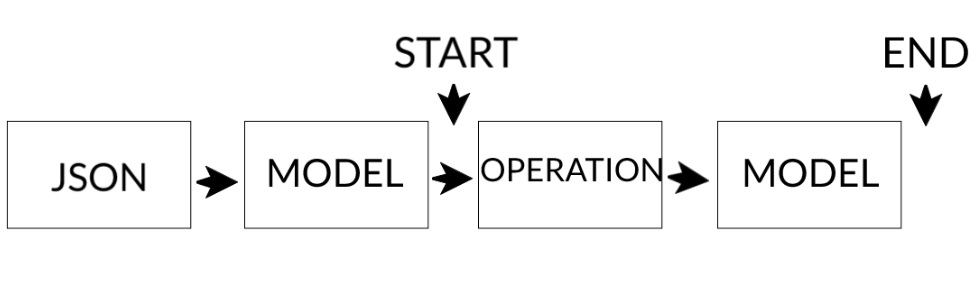
\includegraphics[width=\linewidth]{img/database/operation-scheme.png}
	\caption{Przebieg testów}
	\label{fig: operation_scheme}
\end{figure}

Cały proces testów przedstawia rysunek 5.1.  Pierwszym etapem jest przekształcenie plików w formacie JSON na obiekty programu, których typ jest zależny od wybranej bazy danych. Kolejny z etapów to przekazanie obiektów do odpowiedniej bazy danych i zaczęcie wykonywania operacji, od tego momentu mierzony jest czas operacji. Po wykonaniu operacji otrzymany rezultat operacji przekształcany jest ponownie na obiekty programu i po zakończeniu tej operacji następuje koniec pomiaru czasu operacji. 

W zależności od typu badanej operacji zastosowane zostały różne scenariusze testów. Zależnie od operacji można rozróżnić trzy typy scenariuszy: 

\begin{itemize}
	 \item Zapis danych - w pętli wykonywane są następujące operacje:
	 
	 \begin{enumerate}
	 \item Wygenerowanie danych
	 \item Wyczyszczenie bazy danych
	 \item Wykonanie zapisu danych do bazy
	 \end{enumerate}
	 
	 \item Odczyt danych:
	 
	  \begin{enumerate}
	 \item Wygenerowanie danych
	 \item Wyczyszczenie bazy danych
	 \item Wykonanie zapisu danych do bazy
	 \item W pętli wykonywana zostaje operacja odczytania danych i pomiar czasów
	 \end{enumerate}
	 
	 \item Usuwanie i edycja danych - w pętli wykonywane są następujące operacje:
	 
	 \begin{enumerate}
	 \item Wygenerowanie danych
	 \item Wyczyszczenie bazy danych
	 \item Wykonanie zapisu danych do bazy
	 \item Wykonanie operacji usuwania lub edycji danych i pomiar czasów
	 \end{enumerate}
	 
\end{itemize}

Ilość wykonywania powtórzeń operacji poprzez pętle zostaje zdefiniowana przez użytkownika w ekranie aplikacji widocznym na rysunku \ref{fig: third_app_view}, poprzez wprowadzenie liczby testów w polu tekstowym. Jak można zauważyć najbardziej czasochłonnymi testami jest pomiar czasu edycji i usuwania danych. Podczas tego testu wielokrotnie jest powtarzana operacja zapisu do danych.  

\section{Analiza}

 W~rozdziale zostały przedstawione wyniki przeprowadzonych testów. Dane zostały przedstawione w~tabelach oraz za pomocą wykresów. Każdy z~rezultatów testów został zanalizowany i~opisany.

\subsection{Testy zapisu danych}
 W~podrozdziale zostały przedstawione wyniki testów zapisu danych. Dodatkowo przedstawiono ilość wykorzystanej pamięci operacyjnej podczas operacji oraz stopień wykorzystania procesora. W~systemie iOS nie istnieje możliwość odczytania zajętości pamięci operacyjnej i~zużycia procesora jedynie dla danej operacji. Przedstawione dane pokazują więc parametry dla całej działającej aplikacji. Wyniki te są jak najbardziej miarodajne, gdyż każdy z~testów odbywał się na ''świeżo,, uruchomionej aplikacji. Użycie pamięci operacyjnej i~procesora zawsze miało stały punkt startowy. 

\subsubsection{Mały zestaw danych}

Prezentacja danych w~formie tabel: 

\begin{table}[h]
\centering
\caption{Czasy zapisu danych do bazy - mały zestaw danych}
\label{tab: small-save-time-table}
\begin{tabular}{|c|c|}
\hline
Baza danych   & Czas zapisu [ms] \\ \hline
User Defaults & 2,07             \\ \hline
Realm         & 5,52             \\ \hline
Core Data     & 16,05            \\ \hline
FMDB          & 173,63           \\ \hline
SQLite        & 175,45           \\ \hline
\end{tabular}
\end{table}

\begin{table}[h]
\centering
\caption{Rozmiar pliku wynikowego bazy danych - mały zestaw danych}
\label{tab: small-save-file-size-table}
\begin{tabular}{|c|c|}
\hline
Baza danych   & Rozmiar pliku bazy danych [kb] \\ \hline
User Defaults & 0,04                            \\ \hline
Realm         & 16,38                           \\ \hline
FMDB          & 61,23                           \\ \hline
SQLite        & 61,32                           \\ \hline
Core Data     & 80,04                           \\ \hline
\end{tabular}
\end{table}

\newpage

\begin{table}[h]
\centering
\caption{Użycie procesora podczas operacji - mały zestaw danych}
\label{tab: small-save-cpu-table}
\begin{tabular}{|c|c|}
\hline
Baza danych   & Użycie procesora [\%] \\ \hline
SQLite        & 18                   \\ \hline
FMDB          & 19                   \\ \hline
Realm         & 47                   \\ \hline
Core Data     & 83                   \\ \hline
User Defaults & 88                   \\ \hline
\end{tabular}
\end{table}

\begin{table}[h]
\centering
\caption{Użycie pamięci operacyjnej podczas operacji - mały zestaw danych}
\label{tab: small-save-ram-table}
\begin{tabular}{|c|c|}
\hline
Baza danych   & Użycie pamięci RAM [mb] \\ \hline
User Defaults & 86,4                    \\ \hline
FMDB          & 86,4                    \\ \hline
SQLite        & 86,5                    \\ \hline
Core Data     & 88,6                    \\ \hline
Realm         & 89,7                    \\ \hline
\end{tabular}
\end{table}

\newpage
Prezentacja wyników w~formie wykresów: 

\begin{figure}[h]
\centering
	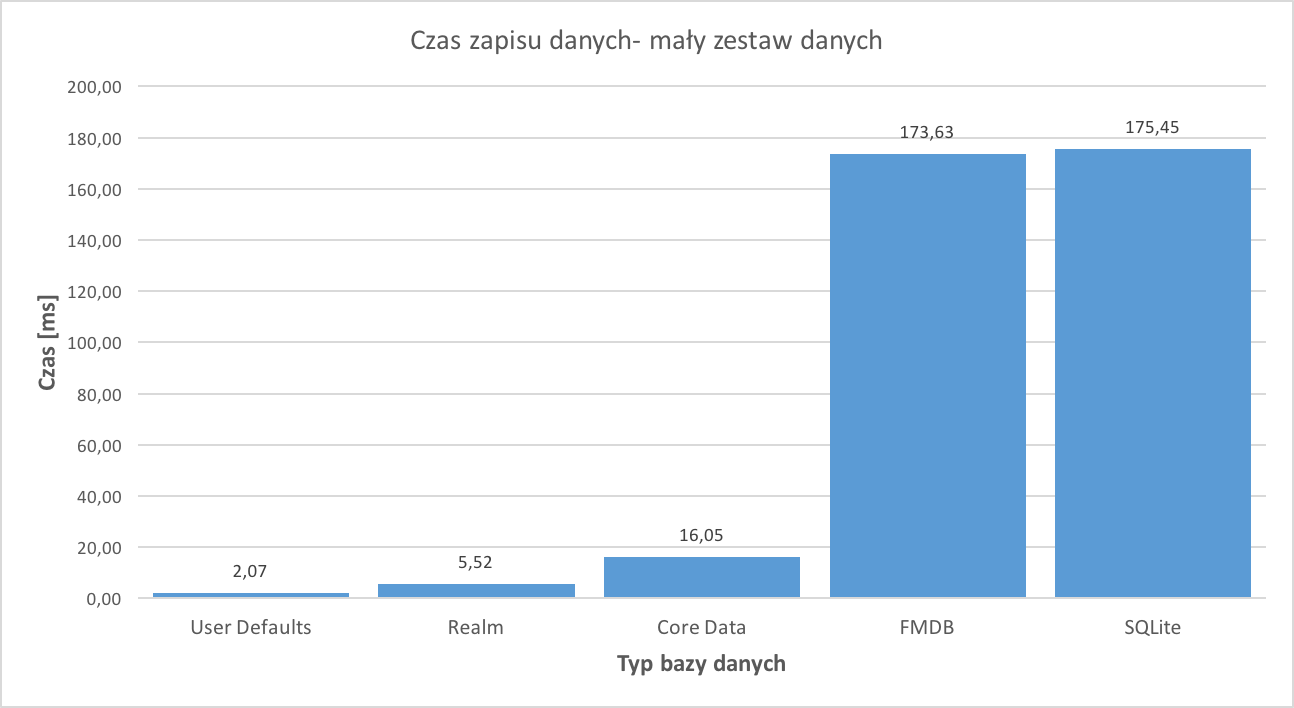
\includegraphics[width=15cm]{img/save_data/save_speed_small.png}
	\caption{Czasy zapisu danych do bazy - mały zestaw danych}
	\label{fig: small-save-time}
\end{figure}

\begin{figure}[h]
\centering
	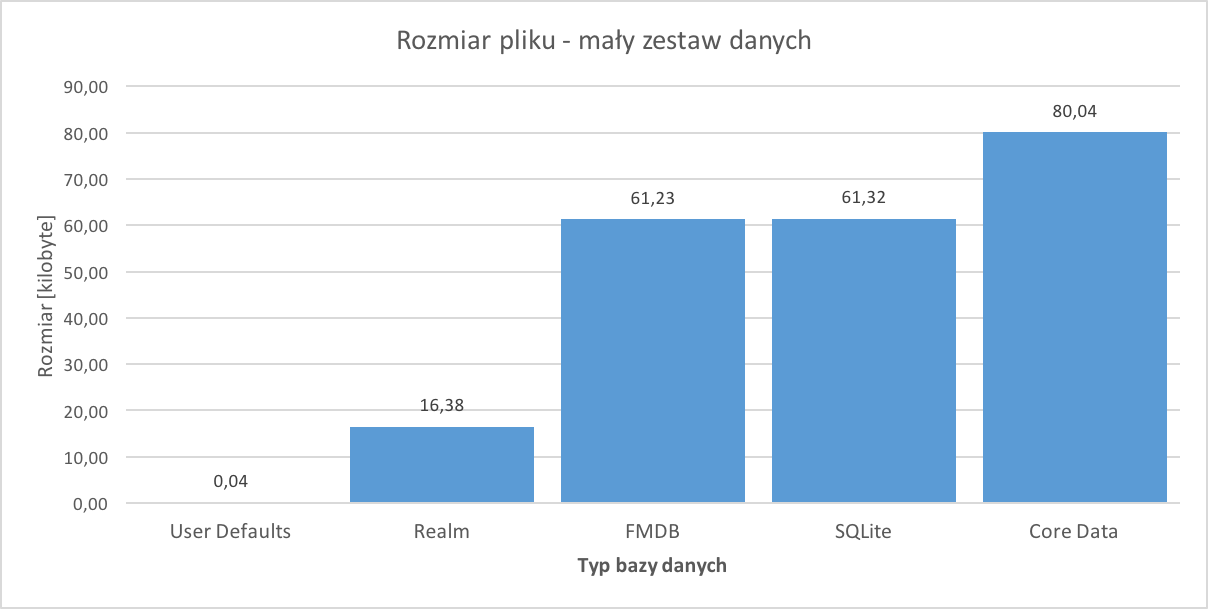
\includegraphics[width=15cm]{img/save_data/save_file_small.png}
	\caption{Rozmiar pliku wynikowego bazy danych - mały zestaw danych}
	\label{fig: small-save-file-size}
\end{figure}

\newpage

\begin{figure}[h]
\centering
	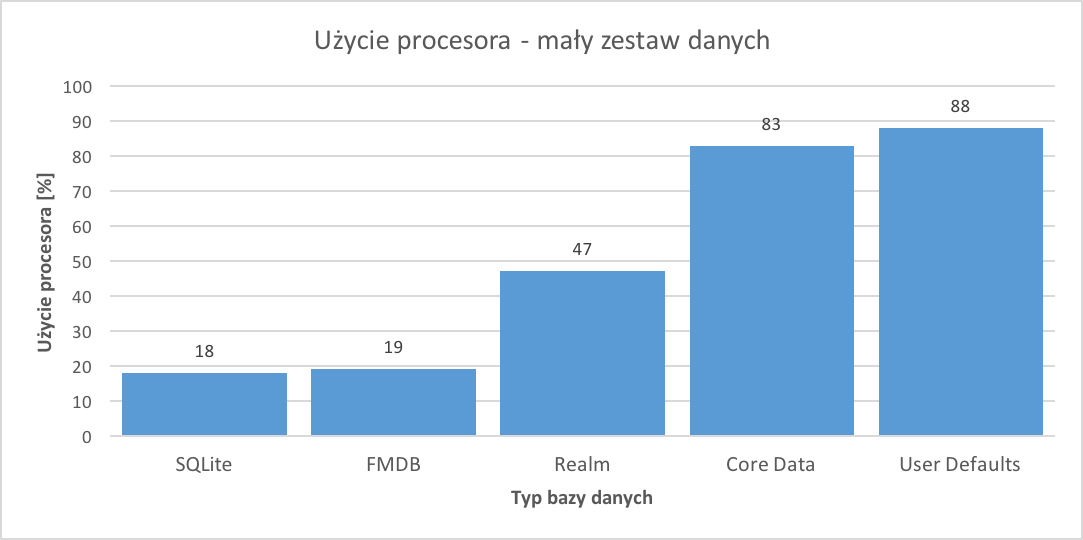
\includegraphics[width=15cm]{img/save_data/save_cpu_small.png}
	\caption{Użycie procesora podczas operacji - mały zestaw danych}
	\label{fig: small-save-cpu}
\end{figure}

\begin{figure}[h]
\centering
	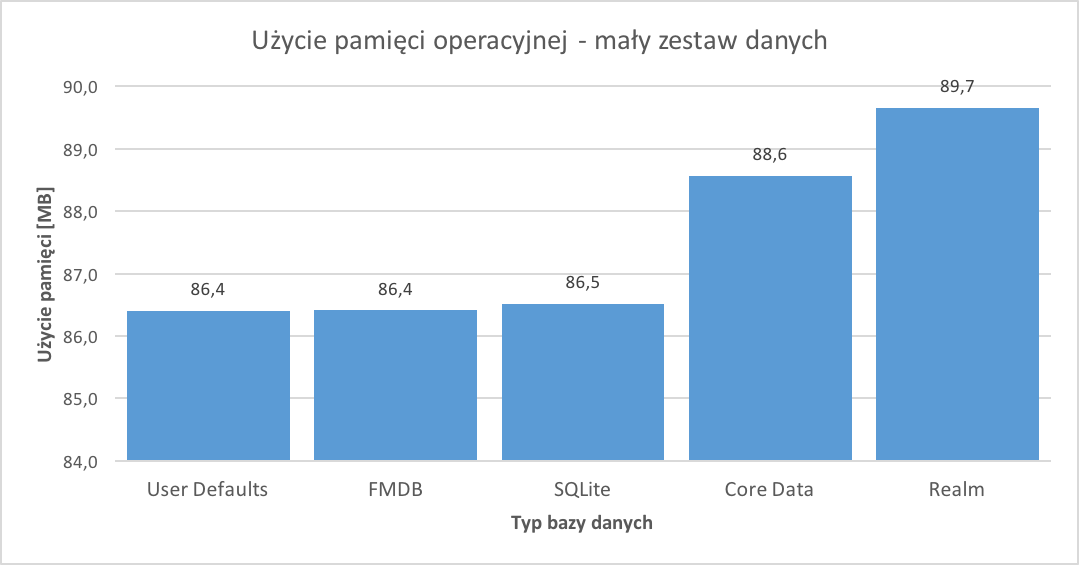
\includegraphics[width=15cm]{img/save_data/save_ram_small.png}
	\caption{Użycie pamięci operacyjnej podczas operacji - mały zestaw danych}
	\label{fig: small-save-ram}
\end{figure}

\newpage

Czasy zapisu danych widoczne na wykresie \ref{fig: small-save-time} i~w tabeli \ref{tab: small-save-time-table} pokazują, że najszybszy okazała się Domyślna Baza Użytkownika, wynika to z~zasady jej działania. Zapisywane są w~niej listy obiektów, nie zachodzi potrzeba ustawiania relacji pomiędzy tabelami. Z~czasem ponad dwukrotnie wyższym wynoszącym 5,52 ms drugi w~kolejności jest Realm. Core Data uzyskała czas trzykrotnie wyższy niż Realm wynoszący 16.05 ms. Najwolniejsze okazały się bazy SQLite i~FMDB uzyskując zbliżone czasy 173,63 ms i~175,45 ms. \par 

Rozmiary plików baz widoczne na wykresie \ref{fig: small-save-file-size} i~w tabeli \ref{tab: small-save-file-size-table} pokazują, że Domyślna Baza Użytkownika posiada najmniejszy rozmiar wynoszący 0.04 kb, przechowuje dane binarne w~wysokim stopniu kompresji. Baza danych Realm posiada plik dużo większy, jego rozmiar wynosi 16,38 kb. SQLite i~FMDB uzyskały niemal równe rozmiary plików. Plik wynikowy Core Data uzyskał rozmiar największy 80 kb. \par

Dane pokazujące użycie procesora podczas operacji zapisu widoczne w~tabeli \ref{tab: small-save-cpu-table} i~na wykresie \ref{fig: small-save-cpu} dowodzą, że SQLite i~FMDB używają jedynie 18-19\% zasobów procesora urządzenia. Realm uzyskuje wynik ponad 50\% wyższy wynoszący 47\%, zaś framework Core Data osiąga aż 83\%. Domyślna Baza Użytkownika, mimo iż uzyskuje najlepszy czas zapisu podczas wykonywania operacji, używa aż 88\% zasobów procesora co jest najgorszym wynikiem.\par 

Podczas testu przy użyciu najmniejszego zestawu danych użycie pamięci operacyjnej urządzenia jest zbliżone dla wszystkich baz danych. Rezultaty widoczne w~tabeli \ref{tab: small-save-ram-table} oscylują w~granicach od 86 mb do 89 mb. Przy tak małej ilości danych różnice te można przyjąć za mało istotne. Kolejne testy pokażą znaczne rozbieżności wykorzystania pamięci RAM pomiędzy testowanymi bazami.

\newpage

\subsubsection{Średni zestaw danych}

Prezentacja danych w~formie tabel: 

\begin{table}[h]
\centering
\caption{Czasy zapisu danych do bazy - średni zestaw danych}
\label{tab: medium-save-time-table}
\begin{tabular}{|c|c|}
\hline
Baza danych   & Czas zapisu [ms] \\ \hline
User Defaults & 4,48             \\ \hline
Realm         & 36,46            \\ \hline
Core Data     & 150,01           \\ \hline
FBDB          & 1872,36          \\ \hline
SQLite        & 1877,78          \\ \hline
\end{tabular}
\end{table}

\begin{table}[h]
\centering
\caption{Rozmiar pliku wynikowego bazy danych - średni zestaw danych}
\label{tab: medium-save-file-size-table}
\begin{tabular}{|c|c|}
\hline
Baza danych   & Rozmiar pliku bazy danych [kb] \\ \hline
User Defaults & 0,08                           \\ \hline
Realm         & 106,99                         \\ \hline
SQLite        & 318,34                         \\ \hline
FBDB          & 326,34                         \\ \hline
Core Data     & 592,94                         \\ \hline
\end{tabular}
\end{table}

\newpage

\begin{table}[h]
\centering
\caption{Użycie procesora podczas operacji - średni zestaw danych}
\label{tab: medium-save-cpu-table}
\begin{tabular}{|c|c|}
\hline
Baza danych   & Użycie procesora [\%] \\ \hline
SQLite        & 16                    \\ \hline
FMDB          & 19                    \\ \hline
Realm         & 77                    \\ \hline
User Defaults & 96                    \\ \hline
Core Data     & 97                    \\ \hline
\end{tabular}
\end{table}

\begin{table}[h]
\centering
\caption{Użycie pamięci operacyjnej podczas operacji - średni zestaw danych}
\label{tab: medium-save-ram-table}
\begin{tabular}{|c|c|}
\hline
Baza danych   & Użycie pamięci RAM [mb] \\ \hline
User Defaults & 91,3                    \\ \hline
FMDB          & 91,4                    \\ \hline
SQLite        & 91,4                    \\ \hline
Realm         & 94,8                    \\ \hline
Core Data     & 102,7                   \\ \hline
\end{tabular}
\end{table}

\newpage

Prezentacja wyników w~formie wykresów: 

\begin{figure}[h]
\centering
	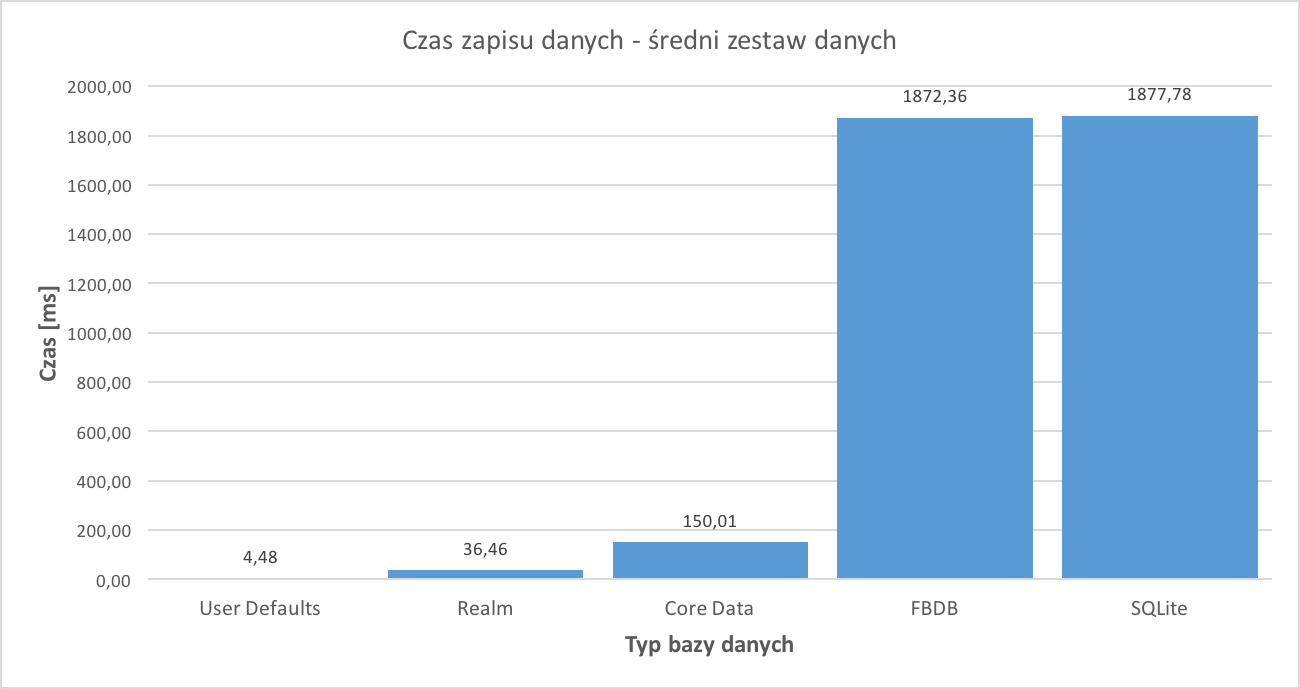
\includegraphics[width=15cm]{img/save_data/save_speed_medium.png}
	\caption{Czasy zapisu danych do bazy - średni zestaw danych}
	\label{fig: medium-save-time}
\end{figure}

\begin{figure}[h]
\centering
	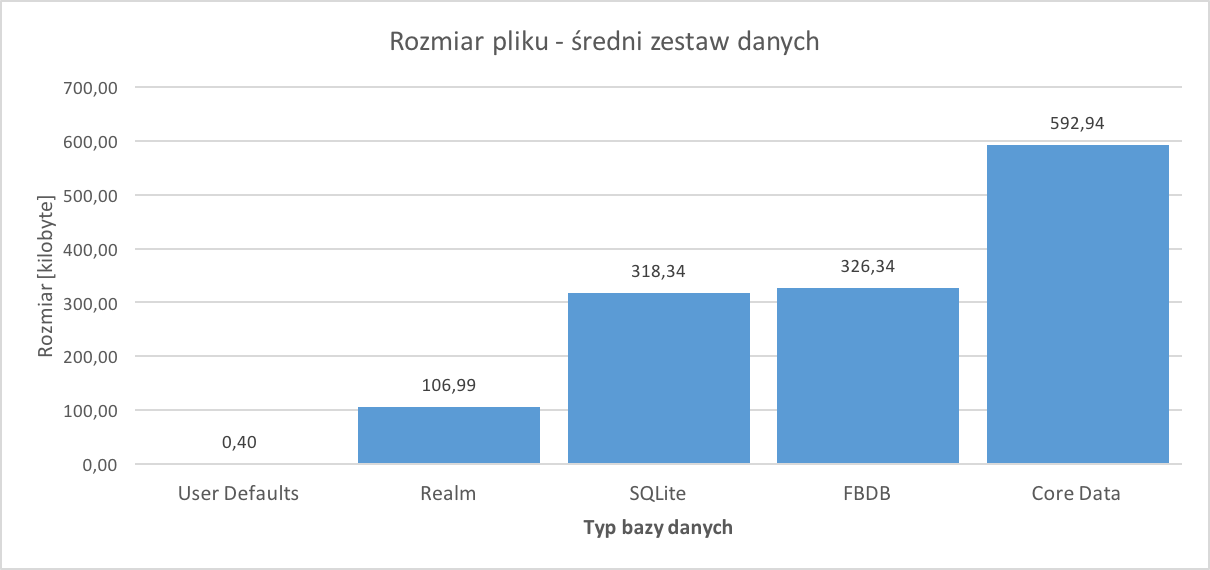
\includegraphics[width=15cm]{img/save_data/save_file_medium.png}
	\caption{Rozmiar pliku wynikowego bazy danych - średni zestaw danych}
	\label{fig: medium-save-file-size}
\end{figure}

\newpage

\begin{figure}[h]
\centering
	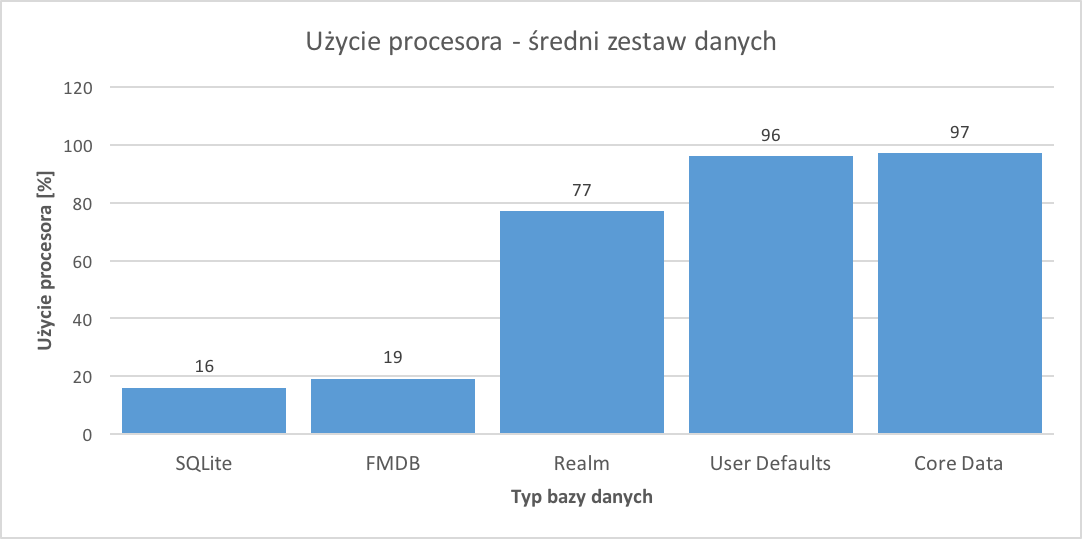
\includegraphics[width=15cm]{img/save_data/save_cpu_medium.png}
	\caption{Użycie procesora podczas operacji - średni zestaw danych}
	\label{fig: medium-save-cpu}
\end{figure}

\begin{figure}[h]
\centering
	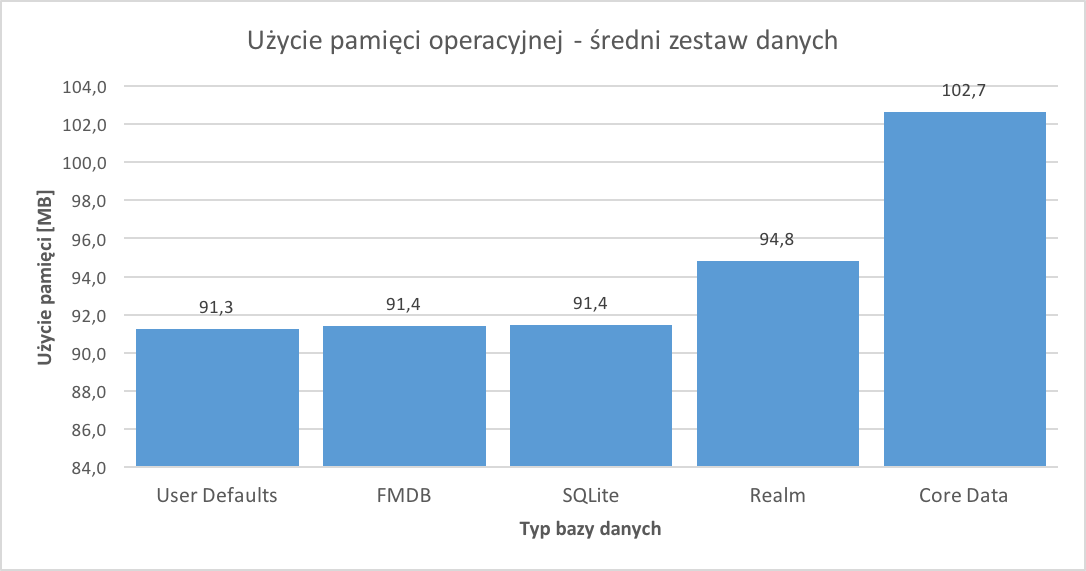
\includegraphics[width=15cm]{img/save_data/save_ram_medium.png}
	\caption{Użycie pamięci operacyjnej podczas operacji - średni zestaw danych}
	\label{fig: medium-save-ram}
\end{figure}

\newpage

Czasy zapisu danych podczas testu ze~średnim zestawem danych  widoczne na wykresie \ref{fig: medium-save-time} pokazały tą samą klasyfikację baz danych co test z~użyciem małego zestawu danych. Czas potrzebny na zapis danych wzrósł o~ponad 50\% dla Domyślnej Bazy Użytkownika, 80\% dla Realm, 85\% dla Core Data. SQLite i~FMDB potrzebowały ponad 90\% czasu więcej, aby zapisać dane średniego zestawu. \par

Podobna sytuacja występuje przy wynikach wielkości plików wynikowych zaprezentowanych na wykresie \ref{fig: medium-save-file-size}. Klasyfikacja baz jest identyczna jak w~poprzednim teście. Plik Domyślnej Bazy Użytkownika osiągnął rozmiar o~90\% większy. Realm, SQLite, FMDB i~Core Data osiągnęły podobny przyrost pliku wynoszący 85\%. \par 

Użycie procesora podczas testu ze~średnim zestawem danych widoczne na wykresie \ref{fig: medium-save-cpu} w~dalszym ciągu dowodzi, że pomimo wzrostu ilości danych SQLite i~FMDB zużywa najmniej zasobów procesora. W~przypadku Realm wykorzystanie CPU wzrosło o~40\%. Core Data i~Domyślna baza użytkownika przy większej ilości danych używały procesora w~96-97\%. \par 

Wykorzystanie pamięci operacyjnej dla SQLite, FMDB i~Domyślnej Bazy Użytkownika wzrosło o~5-6\% co pokazuje wykres \ref{fig: medium-save-ram}. Realm uzyskał lepszy rezultat względem poprzedniego testu, zmniejszając wykorzystanie pamięci RAM o~5\%. Core Data wypadła najgorzej, osiągając 103 MB. \par


\subsubsection{Duży zestaw danych}

Prezentacja danych w~formie tabel: 

\begin{table}[h]
\centering
\caption{Czasy zapisu danych do bazy - duży zestaw danych}
\label{tab: big-save-time-table}
\begin{tabular}{|c|c|}
\hline
Baza danych   & Czas zapisu [ms] \\ \hline
User Defaults & 30,48            \\ \hline
Realm         & 201,93           \\ \hline
Core Data     & 24912,73         \\ \hline
FMDB          & 34217,17         \\ \hline
SQLite        & 35044,62         \\ \hline
\end{tabular}
\end{table}

\newpage

\begin{table}[h]
\centering
\caption{Rozmiar pliku wynikowego bazy danych - duży zestaw danych}
\label{tab: big-save-file-size-table}
\begin{tabular}{|c|c|}
\hline
Baza danych   & Rozmiar pliku bazy danych [kb] \\ \hline
User Defaults & 4,00                           \\ \hline
Realm         & 2588,67                        \\ \hline
SQLite        & 3177,88                        \\ \hline
FMDB          & 3264,30                        \\ \hline
Core Data     & 7240,79                        \\ \hline
\end{tabular}
\end{table}

\begin{table}[h]
\centering
\caption{Użycie procesora podczas operacji - duży zestaw danych}
\label{tab: big-save-cpu-table}
\begin{tabular}{|c|c|}
\hline
Baza danych   & Użycie procesora [\%] \\ \hline
SQLite        & 16                    \\ \hline
FMDB          & 19                    \\ \hline
Realm         & 88                    \\ \hline
Core Data & 98                    \\ \hline
User Defaults    & 97                    \\ \hline
\end{tabular}
\end{table}

\begin{table}[h]
\centering
\caption{Użycie pamięci operacyjnej podczas operacji - duży zestaw danych}
\label{tab: big-save-ram-table}
\begin{tabular}{|c|c|}
\hline
Baza danych   & Użycie pamięci RAM [mb] \\ \hline
SQLite        & 133,2                   \\ \hline
FMDB          & 134,9                   \\ \hline
Realm         & 141,6                   \\ \hline
User Defaults & 145,7                   \\ \hline
Core Data     & 258,5                   \\ \hline
\end{tabular}
\end{table}

\newpage

Prezentacja wyników w~formie wykresów: 

\begin{figure}[H]
\centering
	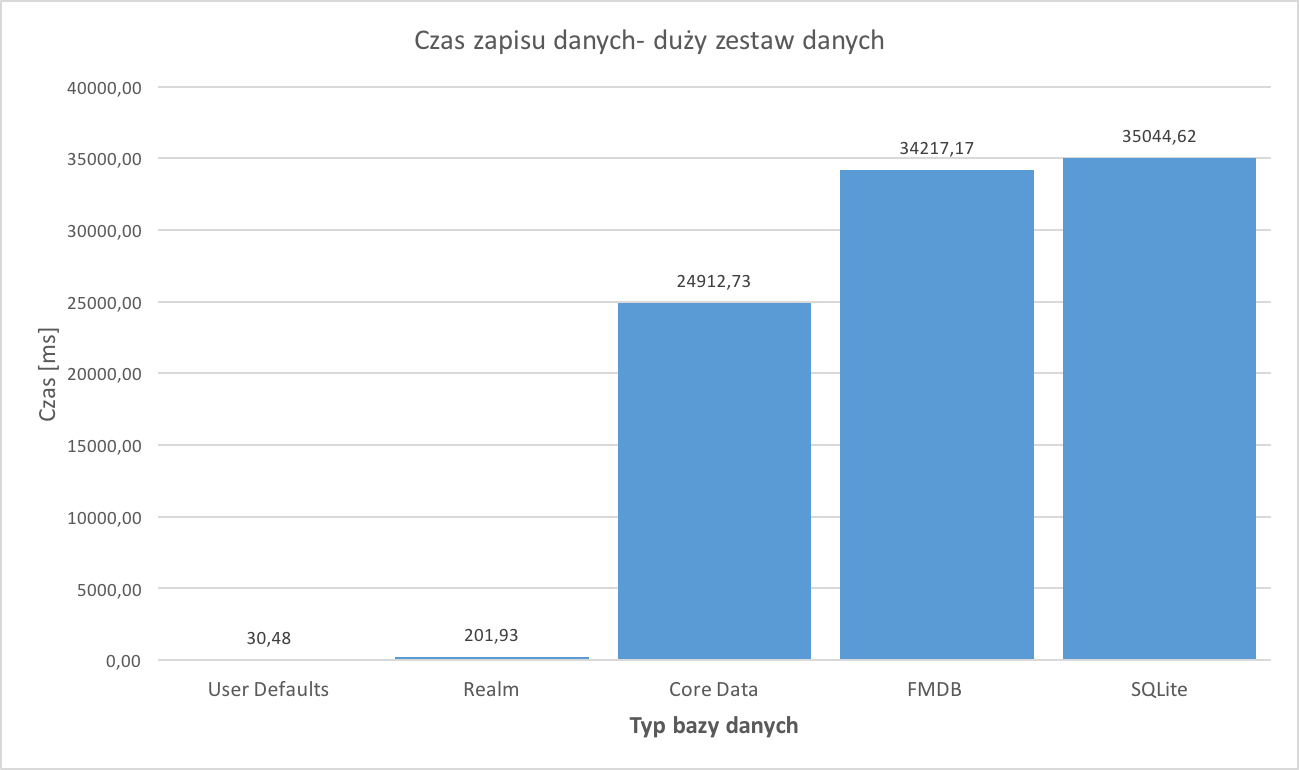
\includegraphics[width=13.5cm]{img/save_data/save_speed_big.png}
	\caption{Czasy zapisu danych do bazy - duży zestaw danych}
	\label{fig: big-save-time}
\end{figure}

\begin{figure}[H]
\centering
	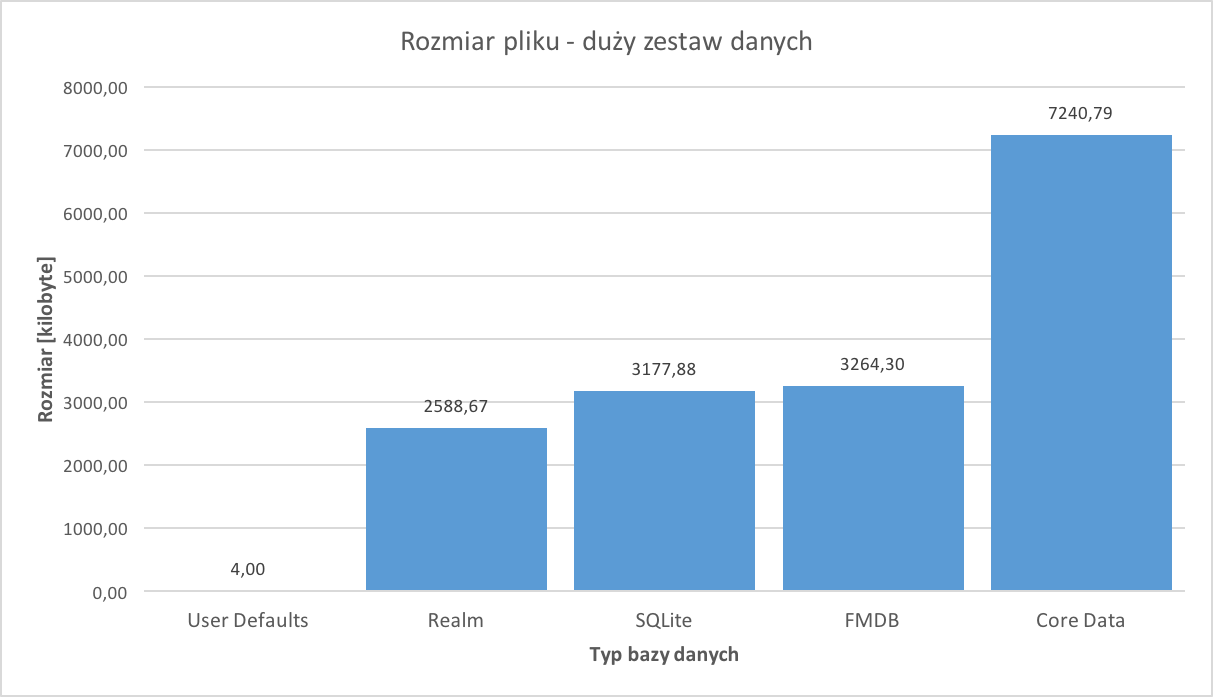
\includegraphics[width=13.5cm]{img/save_data/save_file_big.png}
	\caption{Rozmiar pliku wynikowego bazy danych - duży zestaw danych}
	\label{fig: big-save-file-size}
\end{figure}

\begin{figure}[H]
\centering
	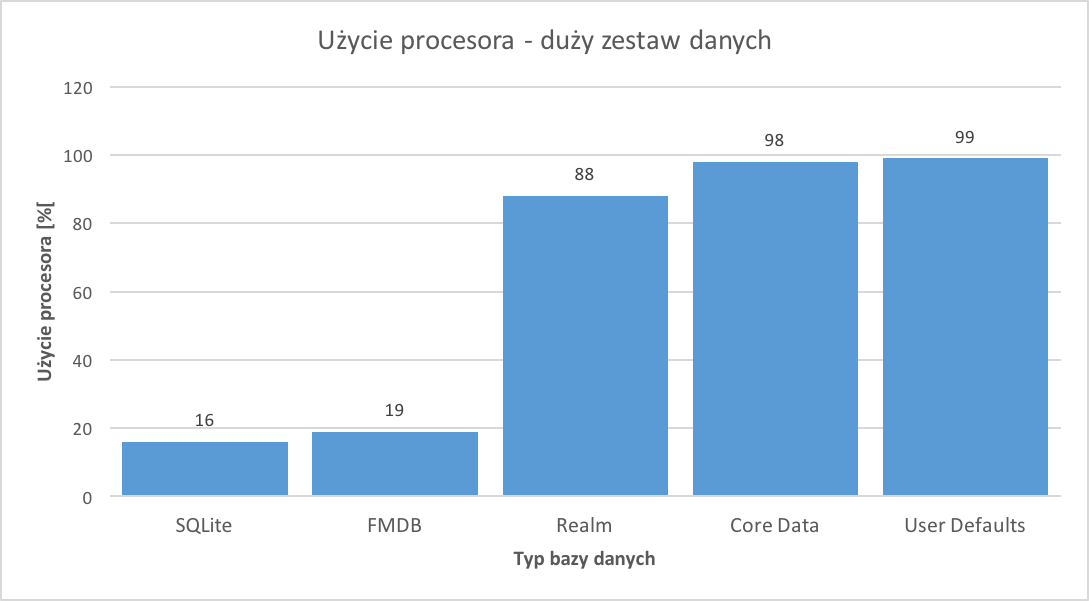
\includegraphics[width=15cm]{img/save_data/save_cpu_big.png}
	\caption{Użycie procesora podczas operacji - duży zestaw danych}
	\label{fig: big-save-cpu}
\end{figure}

\begin{figure}[H]
\centering
	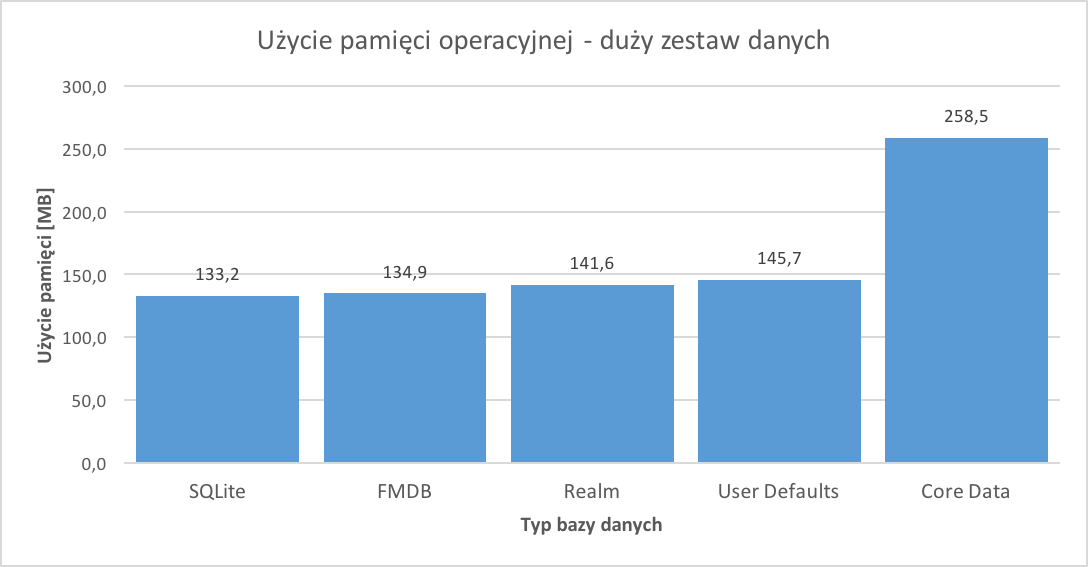
\includegraphics[width=15cm]{img/save_data/save_ram_big.png}
	\caption{Użycie pamięci operacyjnej podczas operacji - duży zestaw danych}
	\label{fig: big-save-ram}
\end{figure}

\newpage

Czasy zapisu danych pokazane na wykresie \ref{fig: big-save-time} udowadniają, że wraz ze wzrostem ilości danych Domyślna Baza Użytkownika i~Realm mają stały przyrost czasu względem dwóch poprzednich testów wynoszący około 85\%. Sytuacja zmienia się w~przypadku pozostałych baz danych. Core Data w~teście z~największym zestawem danych wypada o~wiele gorzej niż w~poprzednich testach. Czas zapisu danych sięga tu 25 sekund. Gorzej względem poprzednich testów wypada SQLite i~FMDB osiągając czasy 34-35 sekund. 

Rozmiary plików wynikowych w~teście z~największą ilością danych widoczny na wykresie \ref{fig: big-save-file-size} pokazują, że Domyślna Baza Użytkownika zwiększa rozmiar wykładniczo względem poprzednich testów. Plik bazy Realm osiąga rozmiar 2588 kb, jest to 25\% więcej niż w~teście ze średnim zestawem danych. FMDB i~SQLite zwiększyły swój rozmiar pliku o~10\% zaś Core Data zwiększyła rozmiar pliku o~12%. 

Użycie procesora podczas testu z~wielkim zestawem danych pokazane na wykresie \ref{fig: big-save-cpu} pokazuje, że w~dalszym ciągu SQLite i~FMDB nie zwiększają zapotrzebowania na moc obliczeniową. Realm w~tym teście potrzebował 10\% wykorzystania procesora. Domyślna Baza Użytkownika i~Core Data pokazały największe zapotrzebowanie wynoszące 98-99\%. 

 W~przypadku użycia pamięci RAM widocznego na wykresie \ref{fig: big-save-ram} można zauważyć, że SQLite i~FMDB posiadają najmniejsze wartości wynoszące 133-135 MB. Realm zachowuje zbliżony rezultat wynoszący 141 MB. Zapotrzebowanie zwiększyła Domyślna Baza Użytkownika, zajmując przedostatnie miejsce z~wartością 145 MB. Core Data zaś potrzebowała aż 258 MB pamięci operacyjnej do operacji zapisu największego zestawu danych, jest to 150\% więcej niż w~poprzednim teście. 

\subsubsection{Podsumowanie - zapis danych}

 Z~testów wynika, że najszybszy zapis danych możliwy jest przy wykorzystaniu Domyślnej Bazy Użytkownika. Realm posiada we wszystkich testach drugi rezultat. Core Data świetnie radzi sobie przy zapisie małej i~średniej ilości danych, natomiast czas zapisu drastycznie rośnie w~przypadku wielkiej liczby danych. SQLite i~FMDB osiągają najgorsze rezultaty, wynikać to może z~surowej implementacji obsługi konwersji danych podczas zapisu. 

 W~wielkości pliku wynikowego także dominuje Domyślna Baza Użytkownika a~zaraz po niej jest Realm. SQLite i~FMDB posiadają pliki niemal tej samej wielkości. Core Data ze względu na zapis do swojego pliku nie tylko samych danych, a~także danych przechowujących graficzną reprezentację bazy oraz wszelkich konfiguracji wykorzystywanych przed środowisko programistyczne XCode osiąga wielkie rozmiary plików wynikowych. 

Najmniejsze zużycie procesora wykazują bazy SQLite i~FMDB. W~przypadku Realm wykorzystanie mocy CPU zależne jest od ilości przetwarzanych danych i~rośnie wraz z~ich ilością. Core Data i~Domyślna Baza Użytkownika wymagają najwięcej zasobów procesora do przeprowadzenia operacji zapisywania danych. 

Wraz ze wzrostem ilości danych rośnie też zapotrzebowanie na pamięć operacyjna urządzenia. W~przypadku małej ilości danych wszystkie bazy wykazują niewielkie zapotrzebowanie na pamięć RAM. Największe różnice widoczne są przy wielkiej ilości danych. Najlepiej w~tej sytuacji radzą sobie bazy SQL, drugie miejsce zajmuje Realm. Core Data wymaga największej  ilości pamięci operacyjnej. 

\subsection{Testy odczytu danych}

Podrozdział przedstawia testy odczytu danych w~kliku różnych scenariuszach: 

\begin{itemize}
\item Odczyt wszystkich danych z~tabel.
\item Wyszukanie wszystkich autorów o~imieniu "Diena".
\item Wyszukanie 2 książek z~największa liczbą autorów.
\item Odczyt maksymalnie 20 wydawnictw z~największą liczba wydanych książek i~posortowanie wyniku rosnąco.
\end{itemize}

Zastosowanie różnych operacji odczytywania danych ma na celu sprawdzenie jak testowane bazy danych radzą sobie podczas wykonywania zapytań. Wykonanie jedynie jednej operacji nie pozwoliłoby uzyskać zadowalających rezultatów, gdyż wiadomo, iż każda z~baz danych inaczej będzie wykonywać każdą z~przeprowadzanych operacji. Tak samo, jak w~przypadku testowania zapisu danych każda z~operacji zostały przeprowadzone na trzech różnych zestawach danych oraz każdy z~testów wykonany został sto razy, a~prezentowany wynik jest średnią z~wszystkich stu operacji. 

\newpage

\subsubsection{Odczyt wszystkich danych}

\begin{figure}[h]
\centering
	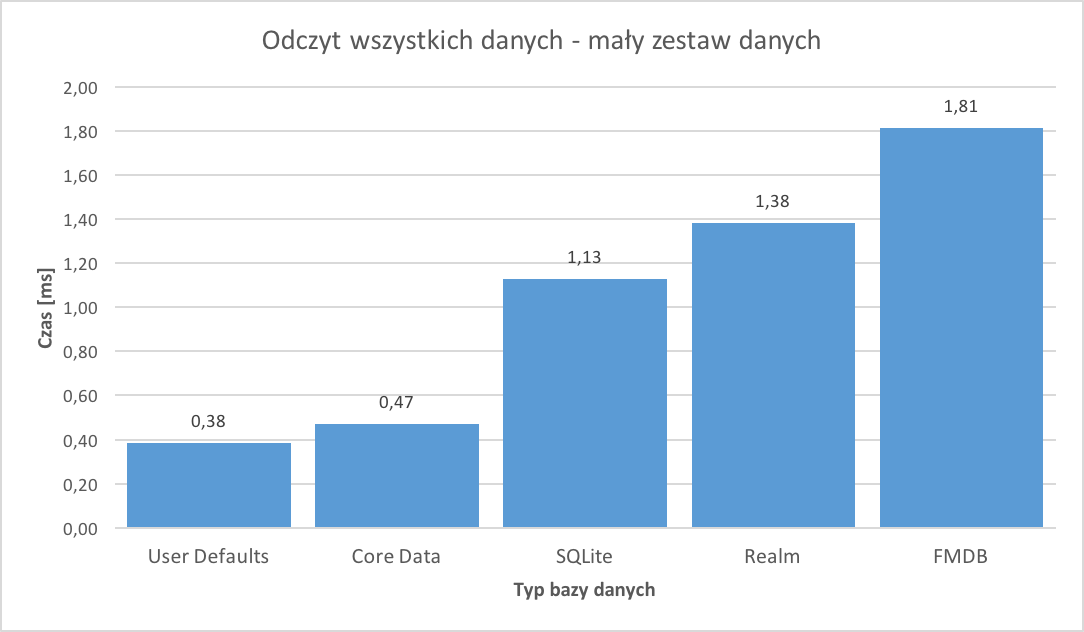
\includegraphics[width=13.5cm]{img/read_data/read_all/read_all_test_small.png}
	\caption{Czas odczytu wszystkich danych - mały zestaw danych}
	\label{fig: read-data-small}
\end{figure}

\begin{figure}[h]
\centering
	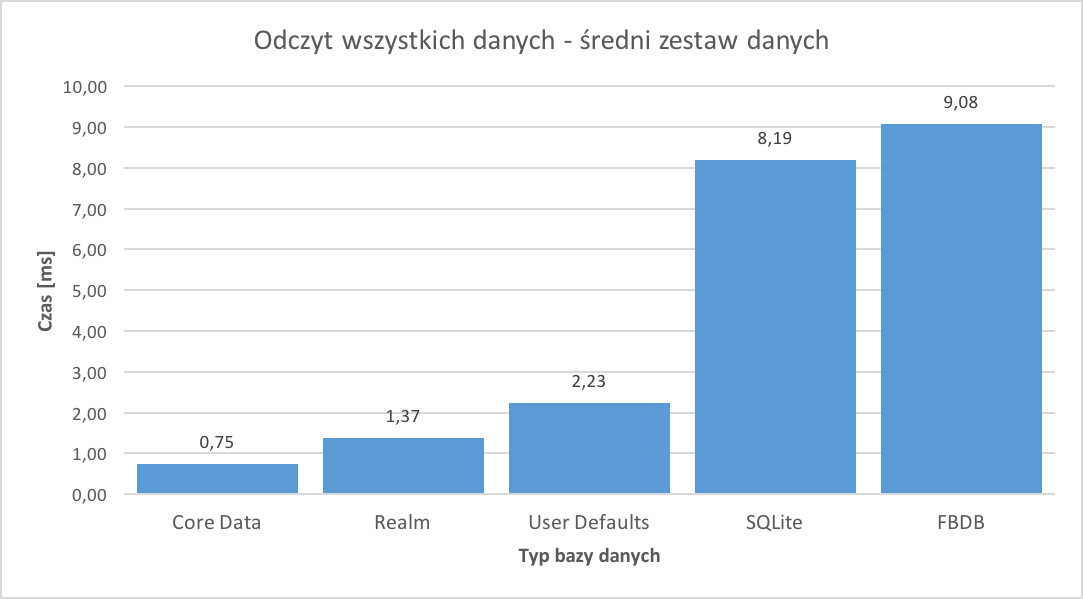
\includegraphics[width=13.5cm]{img/read_data/read_all/read_all_test_medium.png}
	\caption{Czas odczytu wszystkich danych - średni zestaw danych}
	\label{fig: read-data-medium}
\end{figure}

\newpage

\begin{figure}[h]
\centering
	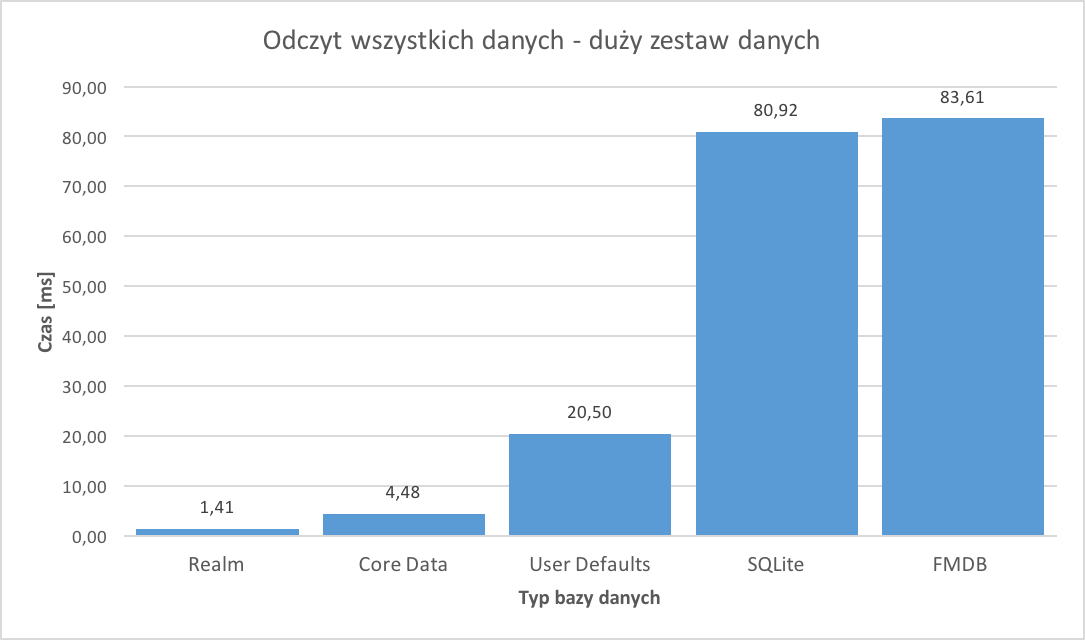
\includegraphics[width=15cm]{img/read_data/read_all/read_all_test_big.png}
	\caption{Czas odczytu wszystkich danych - duży zestaw danych}
	\label{fig: read-data-big}
\end{figure}

Rezultaty odczytu wszystkich danych z~baz prezentują różne wyniki zależne od ilości danych. W~przypadku małego zestawu danych najmniejszy czas równy 0.38 ms uzyskała Domyślna Baza Użytkownika. Zaraz po niej z~czasem 0.47 ms znajduje się Core Data. SQLite uzyskał czas 1.13 ms. Baza danych Realm odczytała wszystkie dane w~czasie 1.38 ms. Najwolniejsza okazała się FMDB dając rezultat 1.81 ms. 

 W~przypadku odczytu średniego zestawu danych najszybsza okazała się Core Data, uzyskując czas 0.75 ms. Realm zaś odczytał dane zestawu średniego w~czasie 1.37 ms, czas ten różnie się zaledwie o~0.01 ms od wyniku uzyskanego przez tą bazę danych przy odczycie małego zestawu danych. Domyślna Baza Użytkownika uzyskała czas 2.23 ms co jest rezultatem gorszym aż o~1.85 względem testu z~użyciem małego zestawu danych. Najwolniejsze okazały się SQLite z~czasem 8,19 ms i~FMDB z~czase 9.08 ms. 

Testy z~użyciem dużego zestawu danych pokazują, że Realm jest najszybszą bazą danych, jeżeli chodzi o~odczyt wszystkich danych znajdujących się w~bazie. Czas odczytu największej ilości danych to zaledwie 1.41 ms. Core Data uzyskała drugi rezultat z~czasem 4.48 ms. Domyślna Baza Użytkownika odczytała dane w~czasie 20.50 ms. SQLite i~FMDB odczytały dane w~najdłuższym czasie wynoszącym ponad 80 ms. 

Można więc zaważyć, że Realm mimo słabych rezultatów w~testach z~małym i~średnim zestawem danych uzyskał doskonały rezultat podczas największego testu. Różnice w~czasach odczytu w~zależności od ilości danych przy użyciu Realm są bardzo niewielkie, wahają się w~granicach 0.04 ms. Domyślna Baza Użytkownika znacząco zwiększa czas odczytu danych wraz ze wzrostem ilości zapisanych danych. Czas odczytu danych w~przypadku użycia Core Data wzrasta wraz ze wzrostem ilości danych, lecz przyrost czasu jest nieduży względem reszty testowanych baz danych. Najwolniejsze i~z największym przyrostem czasowym okazały się bazy SQLite i~FMDB. 

\subsubsection{Wyszukanie wszystkich autorów o~imieniu ''Diena,,}

\begin{figure}[H]
\centering
	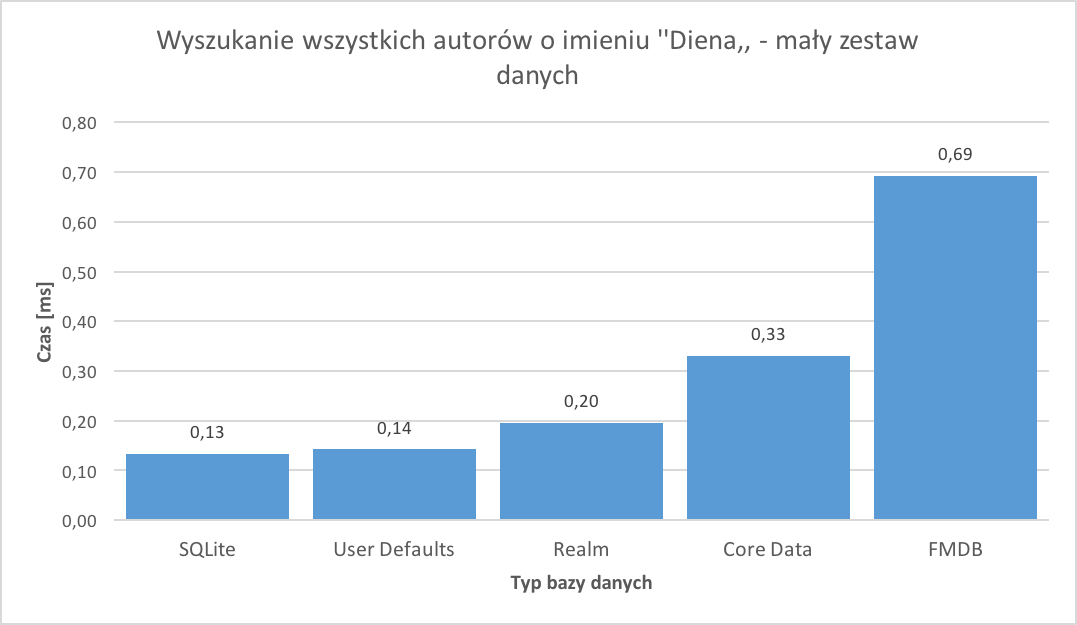
\includegraphics[width=15cm]{img/read_data/read_by_authors/read_by_author_small_test.png}
	\caption{Wyszukanie wszystkich autorów o~imieniu ''Diena,, - mały zestaw danych}
	\label{fig: read-by-author-small}
\end{figure}

\begin{figure}[H]
\centering
	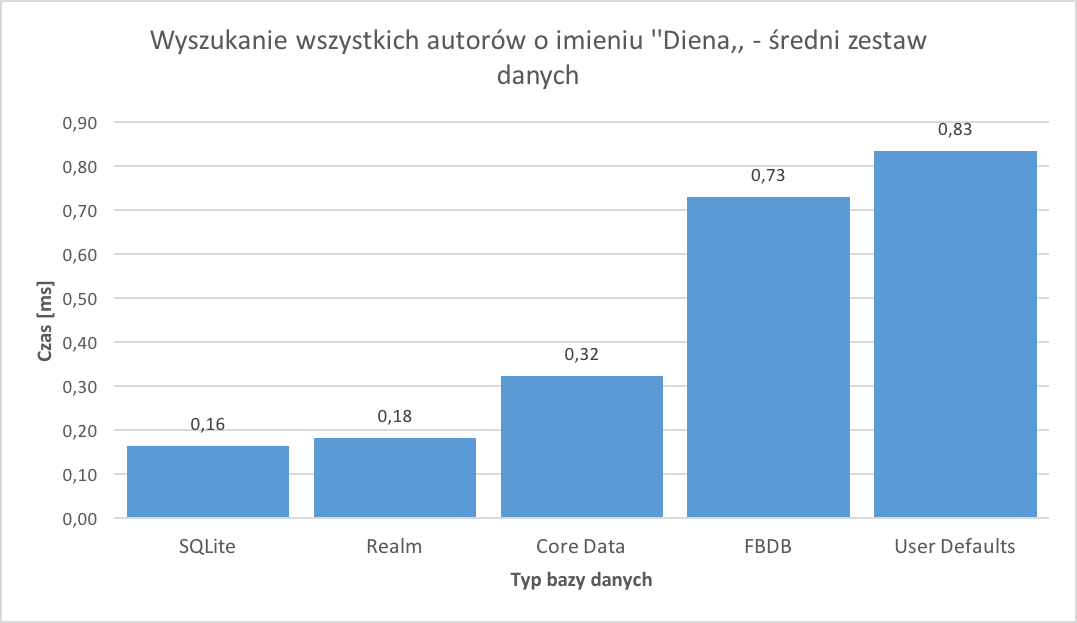
\includegraphics[width=15cm]{img/read_data/read_by_authors/read_by_author_medium_test.png}
	\caption{Wyszukanie wszystkich autorów o~imieniu ''Diena,, - średni zestaw danych}
	\label{fig: read-by-author-medium}
\end{figure}

\begin{figure}[H]
\centering
	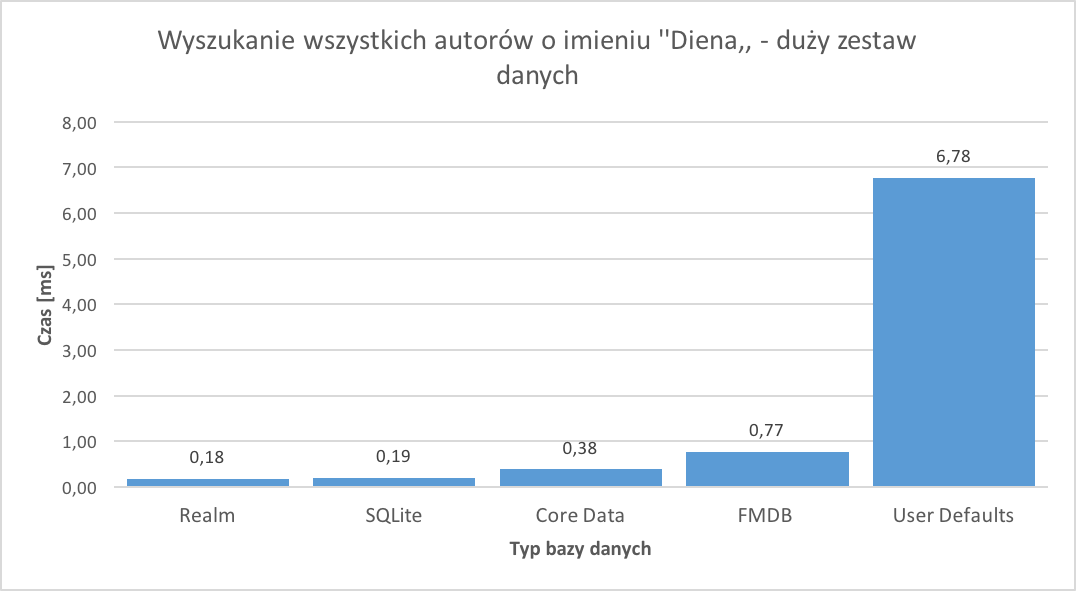
\includegraphics[width=15cm]{img/read_data/read_by_authors/read_by_author_big_test.png}
	\caption{Wyszukanie wszystkich autorów o~imieniu ''Diena,, - duży zestaw danych}
	\label{fig: read-by-author-big}
\end{figure}

Test odczytu autorów o~imieniu ''Diena,, przedstawia następujące wyniki. W~przypadku małego zestawu danych okazał się SQLite z~wynikiem 0.13 ms, na drugim miejscu znalazła się Domyślna Baza Użytkownika uzyskując czas 0.14 ms. Rezultat Realm widoczny na wykresie 6.16 wynosi 0.20 ms, baza ta jest więc wolniejsza o~0.07 ms od najszybszej SQLite. Core Data wyszukała dane w~czasie 0.33 ms. Dobrze widoczna jest różnica w~czasie FMDB od czystej bazy SQLite. Wraper odczytał dane w~czasie 0.69 ms, jest to rezultat gorszy o~0.56 ms od SQLite. 

Odczyt w~przypadku średniego zestawu danych pokazuję, że dziesięciokrotnie większa ilość rekordów względem poprzedniego testu  nie wpływa znacząco na bazy Realm, SQLite, Core Data i~FMDB. Rezultaty widoczne na wykresie \ref{fig: read-by-author-medium} są większe o~0.02 - 0.04 ms. Znaczącą różnicę pokazuję zaś Domyślna Baza Użytkownika, odczytała ona dane w~czasie 0.83 ms co jest rezultatem o~85\% gorszym niż w~poprzednim teście. 

Także odczyt dużego zestawu danych nie wpłyną znacząco na uzyskane czasy otrzymania rezultatów. Na wykresie \ref{fig: read-by-author-big} widać, że tak jak poprzednio czasy dla baz Realm, SQLite, Core Data i~FMDB są większe o~0.02 - 0.04 ms w~porównaniu to poprzedniego testu. Domyślna Baza Użytkownika tak samo zwiększyła swój czas odczytu do 6.78 ms i~jest to rezultat także o~85\% większy niż w~poprzednim teście. 

Przedstawiona operacja odczytu autorów o~wybranym imieniu nie wymagała przetwarzania relacji w~bazach. Można tutaj zauważyć, które z~baz danych dobrze radzą sobie z~prostym przeszukiwaniem zapisanych danych. Realm i~SQLite przetwarzając różne ilości danych, potrzebują bardzo zbliżonego czasu na znalezienie rezultatu zapytania. Core Data, pomimo iż jest blisko dwukrotnie wolniejsza od Realm i~SQLite także nie zwiększa znacząco czasu odczytu względem ilości danych. FMDB, mimo iż jest wraperem SQLite okazuje się jednym z~najwolniejszych rozwiązań. Domyślna Baza Użytkownika radzi sobie znakomicie z~małą ilością danych. Wraz ze wzrostem liczby rekordów czas rośnie o~85\% przy zwiększaniu ilości danych dziesięciokrotnie.

\subsubsection{Wyszukanie 2 książek z~największa liczbą autorów}

\begin{figure}[H]
\centering
	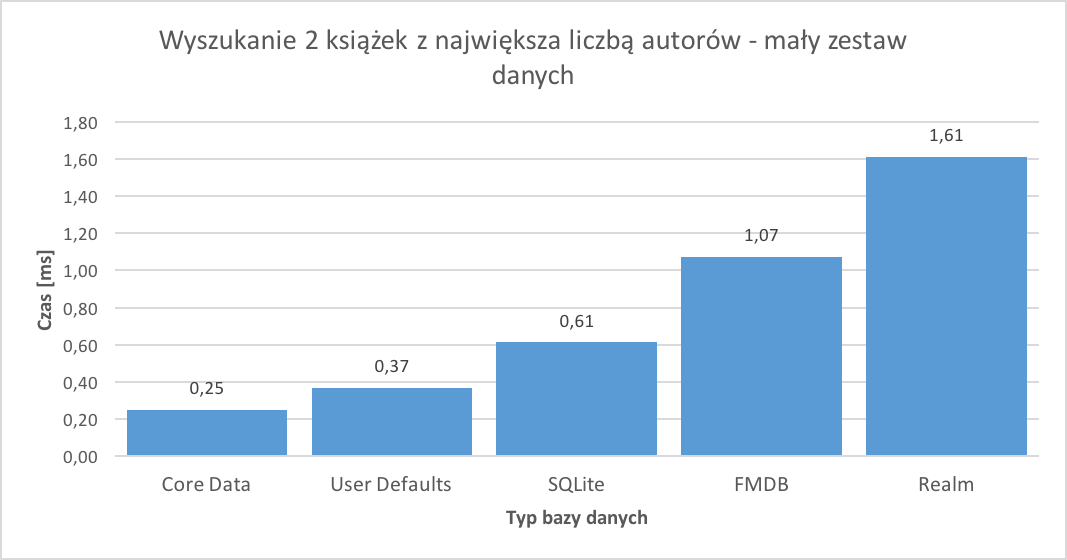
\includegraphics[width=15cm]{img/read_data/read_by_books/read_by_books_small_test.png}
	\caption{Wyszukanie 2 książek z~największa liczbą autorów - mały zestaw danych}
	\label{fig: read-by-books-small}
\end{figure}

\begin{figure}[H]
\centering
	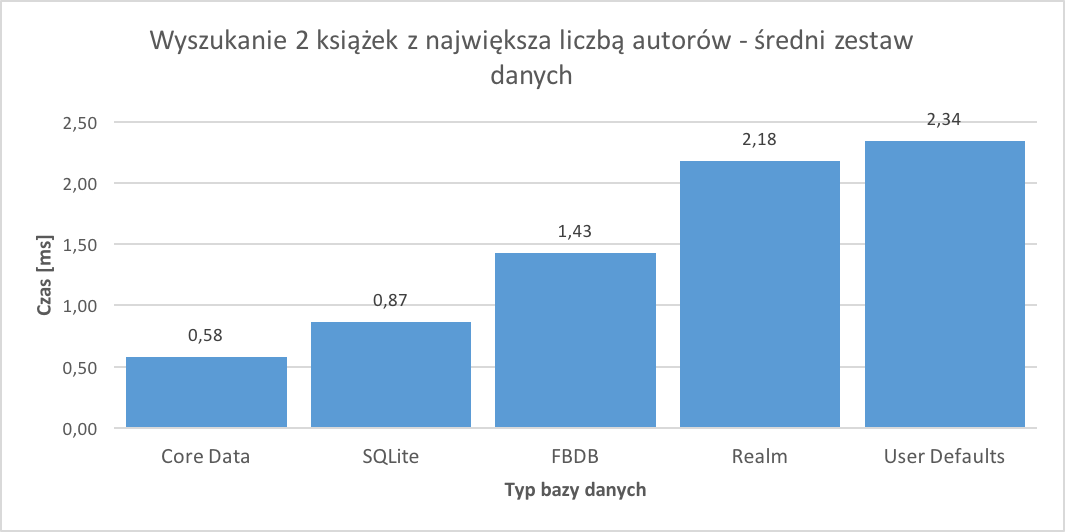
\includegraphics[width=15cm]{img/read_data/read_by_books/read_by_books_medium_test.png}
	\caption{Wyszukanie 2 książek z~największa liczbą autorów - średni zestaw danych}
	\label{fig: read-by-books-medium}
\end{figure}

\begin{figure}[H]
\centering
	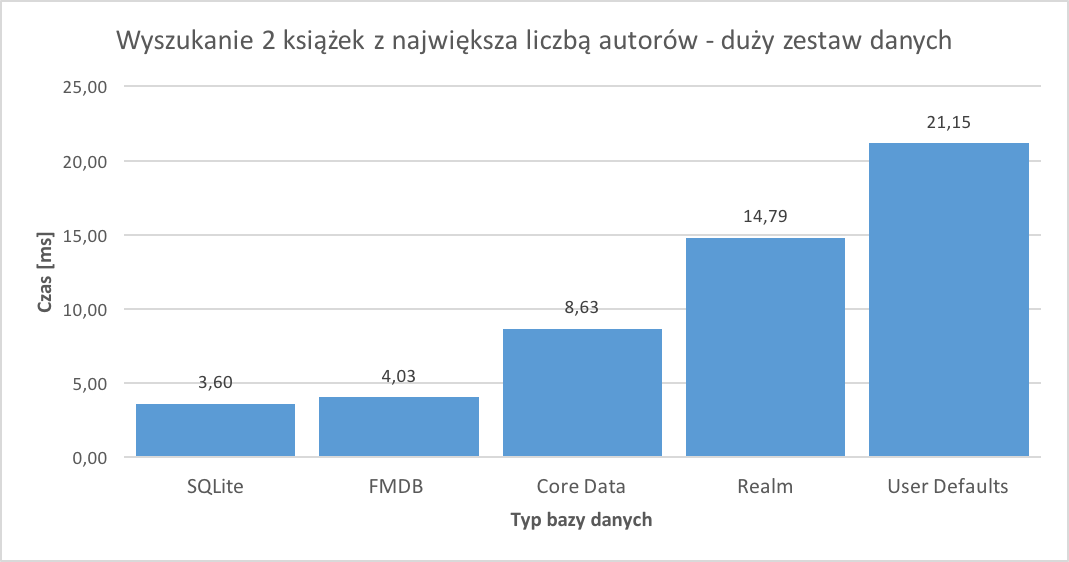
\includegraphics[width=15cm]{img/read_data/read_by_books/read_by_books_big_test.png}
	\caption{Wyszukanie 2 książek z~największa liczbą autorów - duży zestaw danych}
	\label{fig: read-by-books-big}
\end{figure}

Test wyszukania książek z~największą liczbą autorów wymagał wspierania się relacjami pomiędzy tabelami książka i~autor. Wyniki testów pokazują znaczące różnice w~szybkości działania baz w~porównaniu do testu przeszukiwania jednej tabeli. 

Wykres \ref{fig: read-by-books-small} przedstawia rezultaty wyszukanie 2 książek z~największa liczbą autorów w~przypadku użycia małego zestawu danych. Najszybsza okazała się Core Data uzyskując czas równy 0.25 ms. Z~małą ilością danych dobrze poradziła sobie też Domyślna Baza Użytkownika uzyskując rezultat 0.37 ms. Trzeci w~kolejności jest SQLite z~czasem 0.61 ms. Ponownie wolniejszy od SQLite okazał się FMDB, zwrócił on rezultat w~czasie 1.07 ms. Najwolniejsza jest baza Realm, uzyskała ona czas 1.61 ms.

Dane przedstawione na wykresie \ref{fig: read-by-books-medium} pokazują rezultatu testu z~użyciem średniego zestawu danych. Core Data uzyskała najmniejszy czas 0.58 ms jest to rezultat o~55\% większy od testu z~małym zestawem danych. SQLite zakończył zadanie w~czasie 0.87 ms, zaś FMDB ponownie okazał się wolniejszy od SQLite uzyskując czas 1.43 ms. Przedostatni rezultat uzyskał Realm, czas operacji wyniósł 2.18 ms. Domyślna Baza Użytkownika po raz kolejny, podczas zwiększenia ilości danych uzyskuje znacznie gorsze wyniki. Baza zwróciła rezultat w~czasie 2.34 ms i~kolejny raz jest to rezultat większy o~85\% od testu na małym zestawie danych. 

Test z~użyciem dużego zestawu danych, którego wyniki widoczne są na wykresie \ref{fig: read-by-books-big} pokazuje przewagę SQL-a w~operacjach na dużej liczbie danych. Najszybsze okazują się tu bazy SQLite i~FMDB. SQLite uzyskał czas 3.60 ms zaś FMDB 4.03 ms. Trzeci rezultat uzyskała Core Data, potrzebowała ona 90\% czasu więcej niż w~teście poprzednim, lecz w~dalszym ciągu ukończyła zadanie z~dobrym czasem wynoszącym 8.63 ms. Jedną z~najwolniejszych baz okazał się Realm, zrealizował on zapytanie w~czasie 14.79 ms. Najwolniejsza okazała się ponownie Domyślna Baza Użytkownika, uzyskując czas 21.15 ms. 

Powyższy test pokazuję przewagę rozwiązań SQL w~bardziej skomplikowanych operacjach niż przeszukanie jednej tabeli. Rozwiązania takie jak SQLite i~FMDB okazują się wolniejsze w~przypadku małej i~średniej liczby danych, lecz zyskują wiele w~przypadku dużej ilości danych. Core Data uzyskuję czasy coraz większe wraz z~liczbą rekordów, lecz nie jest to tak znacząca różnica, jak w~przypadku Realm czy Domyślnej Bazy Użytkownika, która okazała się najwolniejsza w~przedstawionym teście niezależnie od zestawu danych. 

\subsubsection{Odczyt maksymalnie 20 wydawnictw z~największą liczba wydanych książek oraz posrotowanie wyniku rosnąco}

\begin{figure}[H]
\centering
	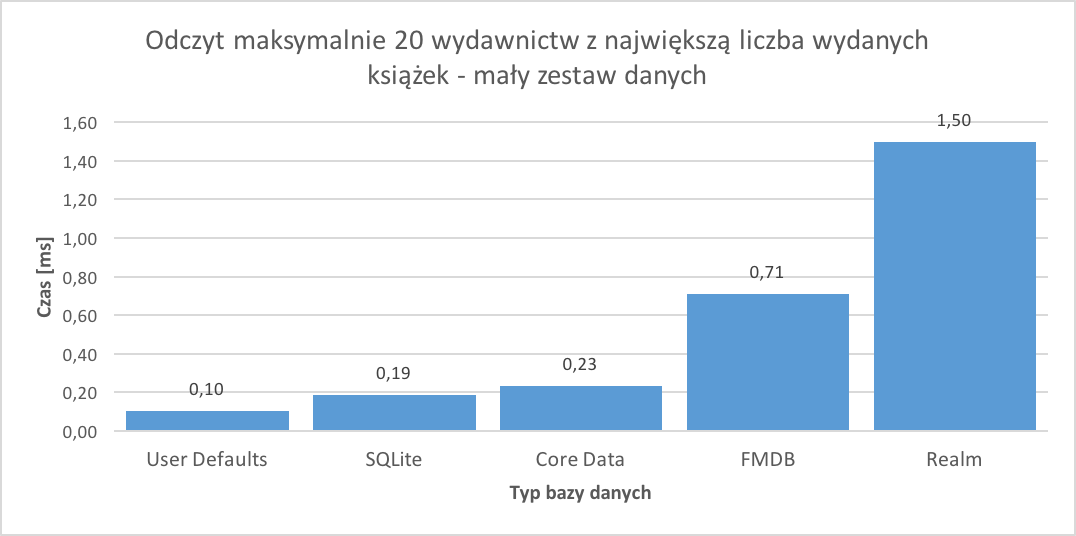
\includegraphics[width=13.5cm]{img/read_data/read_by_publishers/read_by_publishers_small_test.png}
	\caption{Odczyt wydawnictw z~największą liczba wydanych książek - mały zestaw}
	\label{fig: read-by-publishers-small}
\end{figure}

\begin{figure}[H]
\centering
	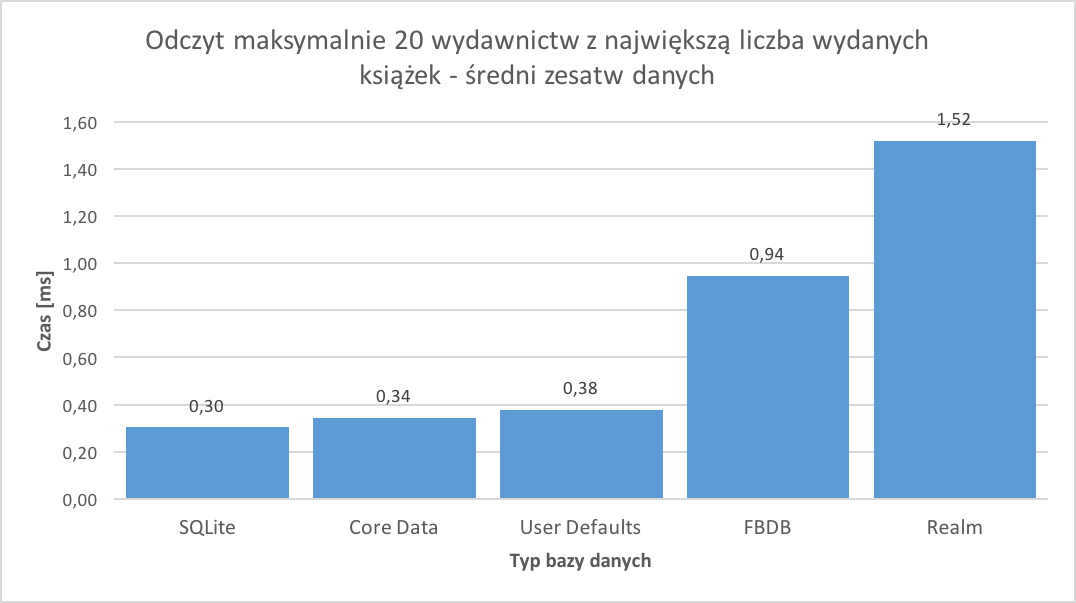
\includegraphics[width=13.5cm]{img/read_data/read_by_publishers/read_by_publishers_medium_test.png}
	\caption{Odczyt wydawnictw z~największą liczba wydanych książek - średni zestaw}
	\label{fig: read-by-publishers-medium}
\end{figure}

\begin{figure}[H]
\centering
	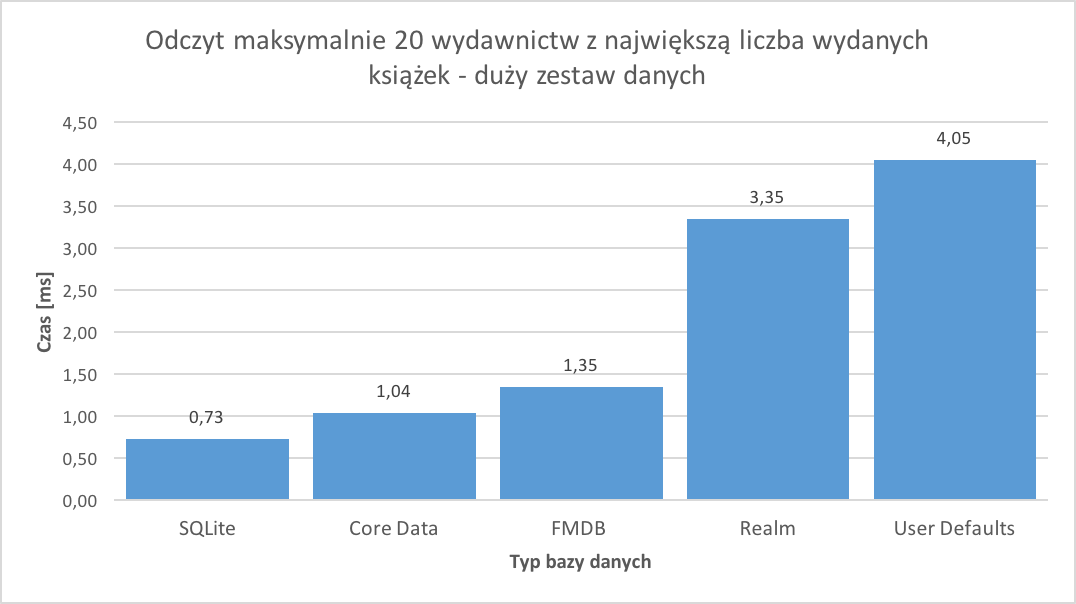
\includegraphics[width=13.5cm]{img/read_data/read_by_publishers/read_by_publishers_big_test.png}
	\caption{Odczyt wydawnictw z~największą liczba wydanych książek - duży zestaw}
	\label{fig: read-by-publishers-big}
\end{figure}

 W~przedstawionym teście zostało dodatkowo dodane sortowanie otrzymanego wyniku. Przy użyciu małego zestawu danych najszybszy czas otrzymania rezultatu uzyskała Domyślna Baza Użytkownika, skończyła wykonywać operacje w~czasie 0.10 ms. Drugi w~kolejności czas należy do SQLite i~wynosi 0.19 ms. O~0.04 ms wolniejsza okazała się Core Data, wykonując operacje w~czasie 0.23 ms. Jednym ze znacznie wolniejszych rozwiązań okazał się FMDB, uzyskał on czas 0.71 ms. Najwolniejszy w~teście okazał się Realm wykonując zadanie w~1.50 ms.\par

Przy użyciu średniego zestawu danych najszybsza jest baza SQLite, wynik otrzymany zostaje w~czasie 0.30 ms. Kolejny raz Core Data jest o~0.04 ms wolniejsza, rezultat zostaje zwrócony po 0.34 ms. Domyślna Baza Użytkownika uzyskała gorszy rezultat niż w~przypadku małego zestawu danych, uzyskała czas 0.38 ms. Przedostatnie miejsce kolejny raz zajmuje FMDB, wykonując operacje w~czasie 0.94 ms. Kolejny raz najwyższy czas należy do Realm wynosi on 1.51 ms i~jest on jedynie o~0.01 ms większy niż w~poprzednim teście.\par

Podczas testów z~wykorzystaniem największego zestawu danych, najlepszy rezultat ponownie należy do SQLite, uzyskał on czas 0.73 ms. Core Data kolejny raz jest za SQLite z~czasem 1.04 ms. Lepszy wynik prezentuje FMDB, wykonując operacje odczytu w~czasie 1.35 ms. Jednym z~wolniejszych rozwiązań jest Realm, zakończenie odczytu nastąpiło w~czasie 3.35 ms. Najwolniejsza jest Domyślna Baza Użytkownika, kończąc operacje w~czasie 4.05 ms. 

Prezentowane wyniki pokazują, że w~przypadku małej ilości danych w~tego typu operacji dobrze spisuje się Domyślna Baza Użytkownika, lecz traci ona swoją wydajność w~przypadku dużych ilości danych. Przy większej ilości danych i~dodatkowych operacjach takich jak sortowanie wyniku znacznie lepiej spisują się rozwiązania SQL (SQLite i~FMDB), a~także Core Data. Dokumentowa baza Realm okazała się najmniej wydajna w~przedstawionym teście. 

\subsection{Testy usuwania danych}

Podrozdział przedstawia testy usuwania danych w~kilku różnych scenariuszach: 

\begin{itemize}
\item Usunięcie wszystkich danych.
\item Usunięcie wszystkich autorów, którzy wydali 3 książki.
\item Usunięcie wydawnictw, które wydały książki o~tytułach "Annie Oakley" lub "Tokyo Zombie (Tky zonbi)".
\end{itemize}

Testu usuwania danych przedstawiają różne stopnie skomplikowania operacji. Usunięcie wszystkich danych jest standardowym czyszczeniem bazy danych, podczas którego czyszczone są wszystkie rekordy we wszystkich tablicach. Usunięcie wszystkich autorów, którzy wydali 3 książki, jest to operacja wymagająca zliczenia książek i~wybraniu odpowiednich rekordów do usunięcia. Usunięcie wydawnictw, które wydały książki o~tytułach "Annie Oakley" lub "Tokyo Zombie (Tky zonbi)" wymaga przeszukania relacji jeden do wielu wydawnictwo - książka, porównaniu nazw i~usunięciu odpowiednich rekordów z~tablicy wydawnictwo. 

\subsubsection{Usunięcie wszystkich danych}

\begin{figure}[H]
\centering
	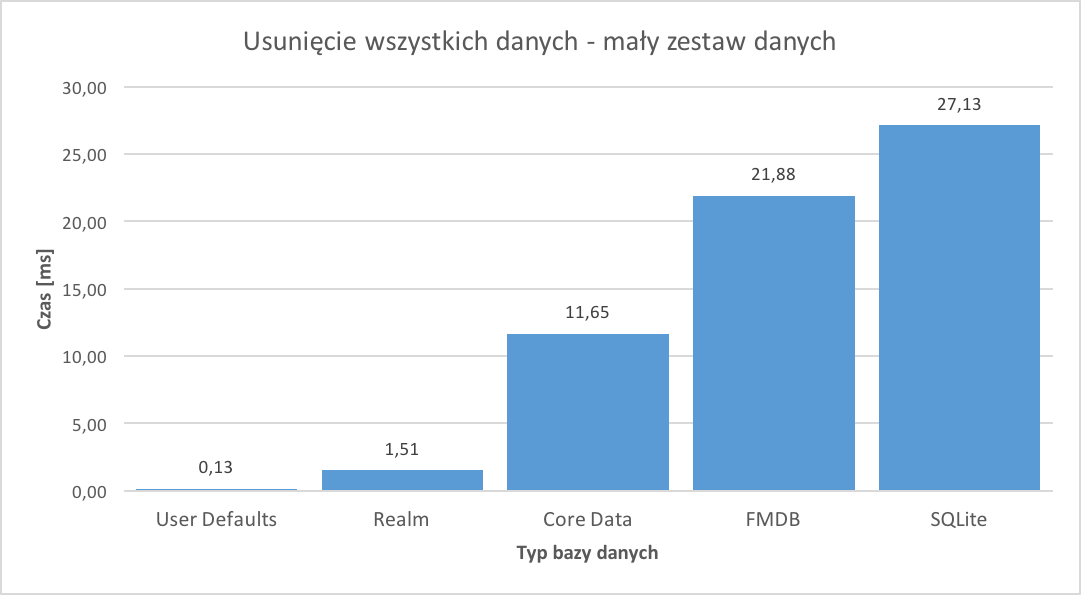
\includegraphics[width=15cm]{img/delete_data/delete_all/delete_all_small_test.png}
	\caption{Usunięcie wszystkich danych - mały zestaw}
	\label{fig: delete-all-small}
\end{figure}

\begin{figure}[H]
\centering
	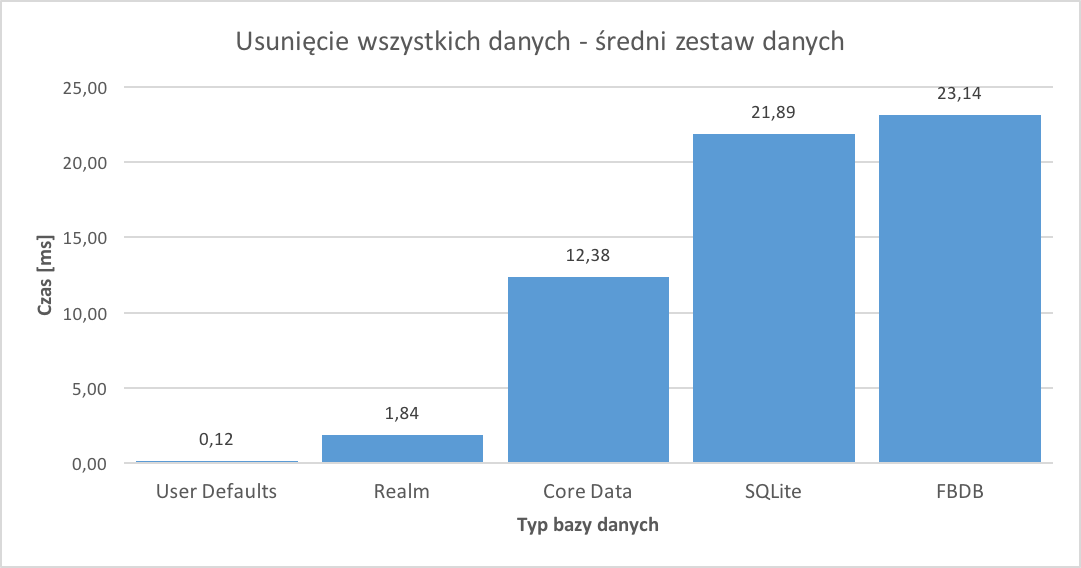
\includegraphics[width=15cm]{img/delete_data/delete_all/delete_all_medium_test.png}
	\caption{Usunięcie wszystkich danych- średni zestaw}
	\label{fig: delete-all-medium}
\end{figure}

\begin{figure}[H]
\centering
	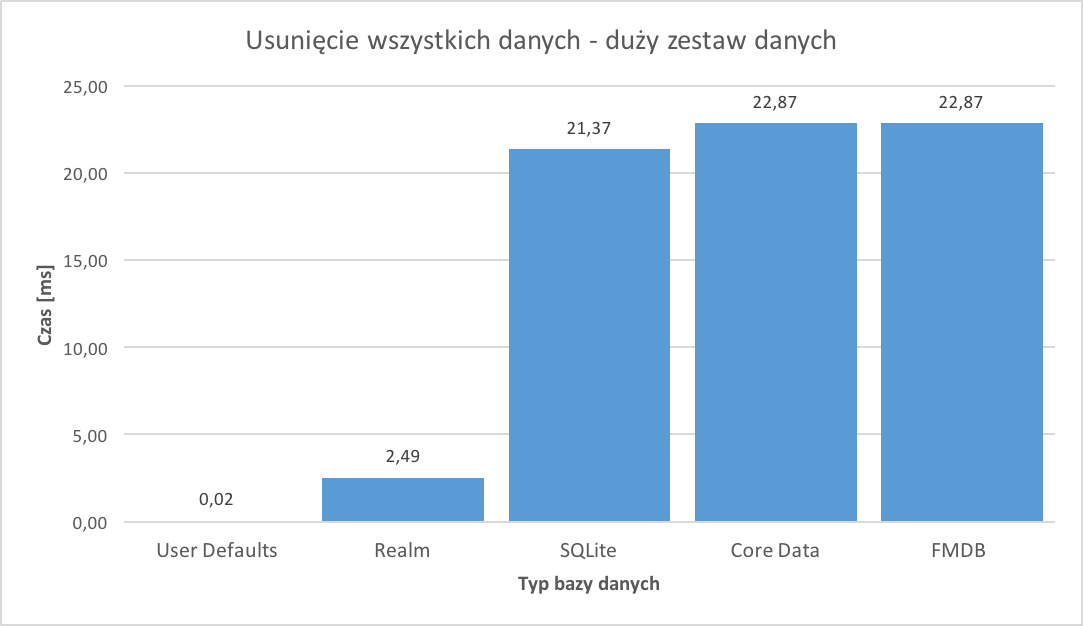
\includegraphics[width=15cm]{img/delete_data/delete_all/delete_all_big_test.png}
	\caption{Usunięcie wszystkich danych - duży zestaw}
	\label{fig: delete-all-big}
\end{figure}

Usunięcie wszystkich danych przy małym zestawie danych pokazuje, że najszybsza jest Domyślna Baza Użytkownika, operacja zakończyła się po 0.13 ms. Realm uzyskał drugi czas wynoszący 1.51 ms. Core Data uzyskała rezultat znacznie wyższy od poprzednich dwóch baz danych i~usunęła dane w~czasie 11.65 ms. Najgorzej wypadły bazy SQL, FMDB wyczyścił tablice w~czasie 21.88 ms. Najwolniejszy był SQLite uzyskując czas 27.13 ms. 

Test przeprowadzony na średnim zestawie danych kolejny raz pokazuję, że najszybsza jest Domyślna Baza Użytkownika, uzyskała ona czas 0.12 ms. Drugi czas ponownie osiąga Realm i~jest on równy 1.84 ms. Core Data także w~tym teście znacząco wolniej usuwa dane, czas wyniósł 12.38 ms. SQLite wraz ze wzrostem ilości danych osiągnął rezultat lepszy niż w~poprzednim teście i~ukończył operacje w~21.89 ms. Najwolniejszy tym razem jest FMDB uzyskując czas 23.14 ms. 

 W~przypadku dużego zestawu danych ponownie najlepszy rezultat należy do Domyślnej Bazy Użytkownika wynosi on 0.02 ms. Ponownie też Realm jest na drugim miejscu, uzyskując czas 2.49 ms. SQLite w~porównaniu do poprzedniego testu wykonał operacje szybciej, pomimo większej ilości danych. Czas uzyskany przez SQLite wynosi 21.37 i~jest o~0.51 mniejszy niż przy użyciu średniego zestawu danych. Różnica ta wynika z~obecnego stanu urządzenia, można więc przyjąć, że operacja wykonana została w~takim samym czasie. Core Data i~FMDB uzyskały takie same czasy wynoszące 22.87 ms. 

Test pokazuje, że niezależnie od zestawu danych najszybsza podczas usuwania wszystkich danych jest Domyślna Baza Użytkownika. Szybki jest też Realm, jego czasy w~stosunku do zwiększającej się ilości danych nie rosną znacząco. SQLite ponownie pokazuję, że doskonale radzi sobie podczas dużej ilości danych, zaś jego wydajność podczas niewielkiej ilości rekordów nie jest zadowalająca. Rezultaty Core Data są zależne od ilości danych i~wydajność bazy spada wraz ze wzrostem ilości rekordów. Najwolniejszy w~teście okazał się wraper FMDB, zaprezentował on najmniejszą wydajność podczas testów. 

\subsubsection{Usunięcie wszystkich autorów którzy wydali 3 książki}

\begin{figure}[H]
    \centering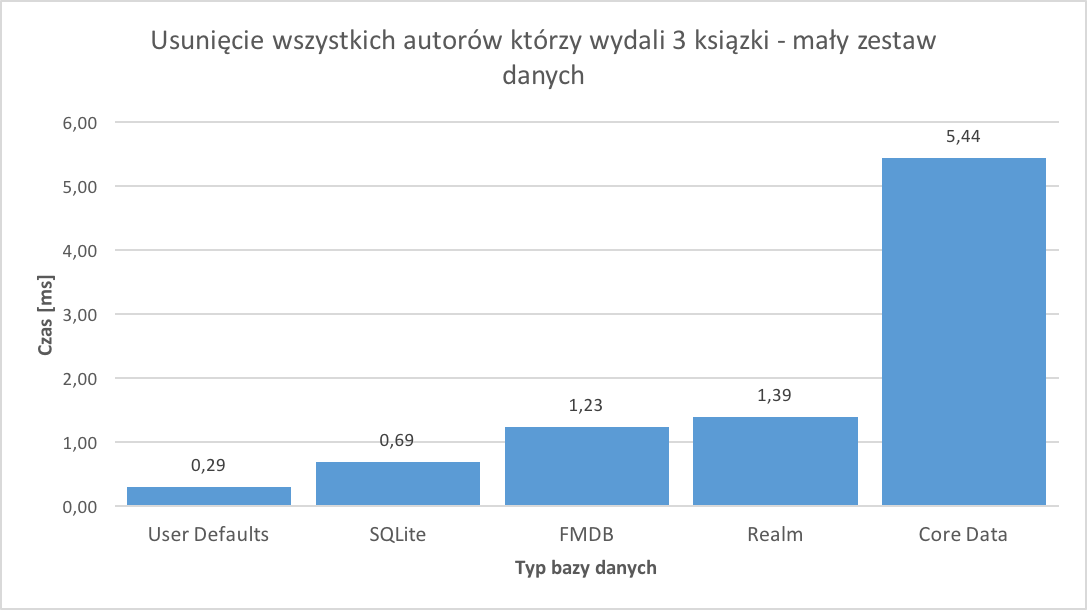
\includegraphics[width=\linewidth]{img/delete_data/delete_by_author/delete_by_author_small_test.png}
    \caption{Usunięcie wszystkich autorów, którzy wydali 3 książki - mały zestaw danych}
    \label{img: delete-by-author-small}
\end{figure}

\begin{figure}[H]
    \centering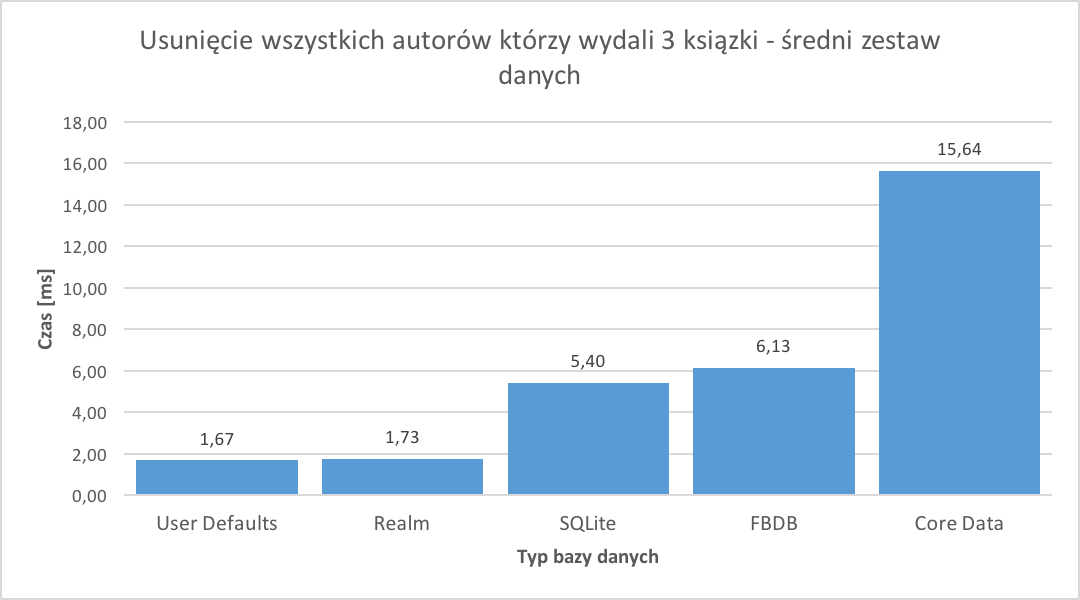
\includegraphics[width=\linewidth]{img/delete_data/delete_by_author/delete_by_author_medium_test.png}
    \caption{Usunięcie wszystkich autorów, którzy wydali 3 książki - średni zestaw danych}
    \label{img: delete-by-author-medium}
\end{figure}

\begin{figure}[H]
    \centering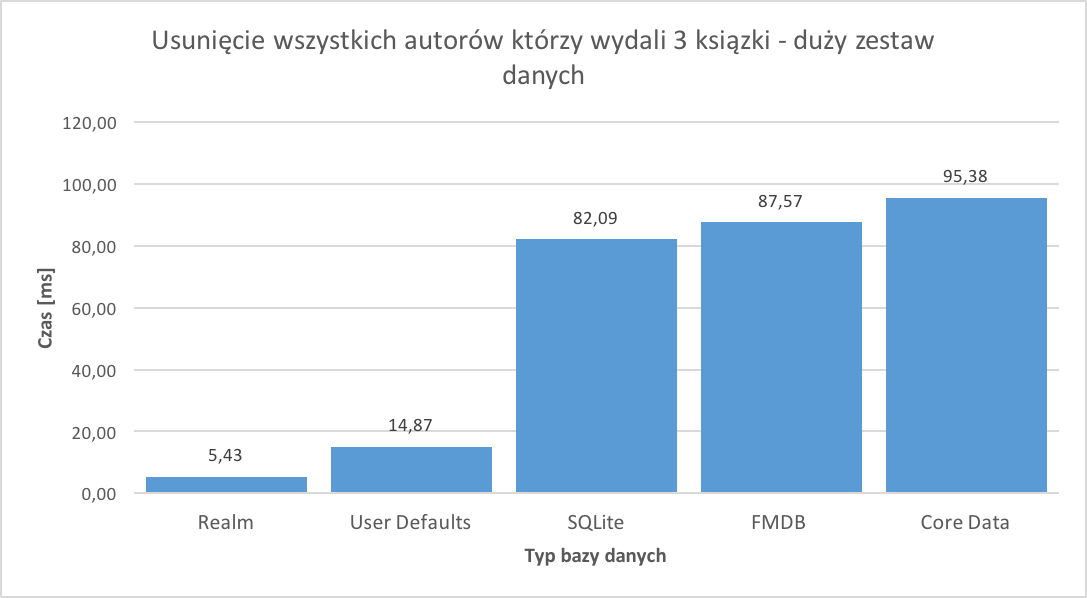
\includegraphics[width=\linewidth]{img/delete_data/delete_by_author/delete_by_author_big_test.png}
    \caption{Usunięcie wszystkich autorów, którzy wydali 3 książki - duży zestaw danych}
    \label{img: delete-by-author-big}
\end{figure}

Wyniki testów usunięcia wszystkich autorów, którzy wydali 3 książki w~przypadku użycia małego zestawu danych widoczne są na wykresie \ref{img: delete-by-author-small}.  Najniższy czas wynoszący 0.29 ms uzyskała Domyślna Baza Użytkownika. Drugi co do wielkości czas należy do SQLite, który uzyskał 0.69 ms. FMDB uzyskał blisko dwukrotnie wyższy czas wynoszący 1.23 ms. Realm zaś ukończył operacje z~czasem gorszym o~0.16 ms od FMDB równym 1.39 ms. Najwolniejsza okazała się Core Data, wykonała ona operacje po upływie 5.44 ms. 

Wyniki testów z~użyciem średniego zestawu danych widoczne są na wykresie \ref{img: delete-by-author-medium}. Najniższy czas równy 1.67 ms ponownie uzyskała Domyślna Baza Użytkownika. Wolniejszy o~0.06 ms okazał się Realm, kończąc zadanie w~czasie 1.73 ms. SQLite zakończył operacje w~czasie 5.40 ms. FMDB zakończyło zadanie w~czasie 6.13 ms. Najwolniejsza ponownie była Core Data, uzyskując czas 15.64 ms.

Rezultaty testów z~wykorzystaniem dużego zestawu danych widoczne są na wykresie \ref{img: delete-by-author-big}. Najszybszy okazał się Realm uzyskując czas 5.43 ms. Drugi co do wielkości rezultat wynoszący 14.87 ms należy do Domyślnej Bazy Użytkownika. SQlite ukończył wykonywanie zadanie w~82.09 ms. FMDB okazał się wolniejszy od SQLite o~5.48 ms i~wykonał operacje w~87.57 ms. Ponownie najwolniejsza okazała się Core Data, uzyskując czas 95.38 ms.

Przedstawiony test wymagał zliczenia wszystkich książek dla każdego z~autorów, a~następnie wybraniu tych, którzy wydali trzy książki i~usunięciu ich z~bazy. Wyniki pokazują, że przy małej i~średniej ilości danych w~tego typu operacjach, dobrze spisuję się Domyślna Baza Użytkownika, która radzi sobie gorzej w~przypadku dużej ilości danych. Realm w~przypadku małej i~średniej ilości danych wykonuje zadanie w~podobnym czasie, różnica wynosi jedynie 0.34 ms, zaś ta baza danych prezentuje doskonały rezultat w~przypadku dużej ilości danych i~jest najszybsza z~testowanych baz. SQLite i~FMDB nie pokazują zaskakującej wydajności w~tego typu operacjach. FMDB przy użyciu różnych zestawów danych zawsze wypada gorzej od SQLite. Core Data okazała się najwolniejszym rozwiązaniem.

\subsubsection{Usunięcie wydawnictw które wydały książki o~tytułach ,,Annie Oakley'' lub ,,Tokyo Zombie (Tky zonbi)''}

\begin{figure}[H]
    \centering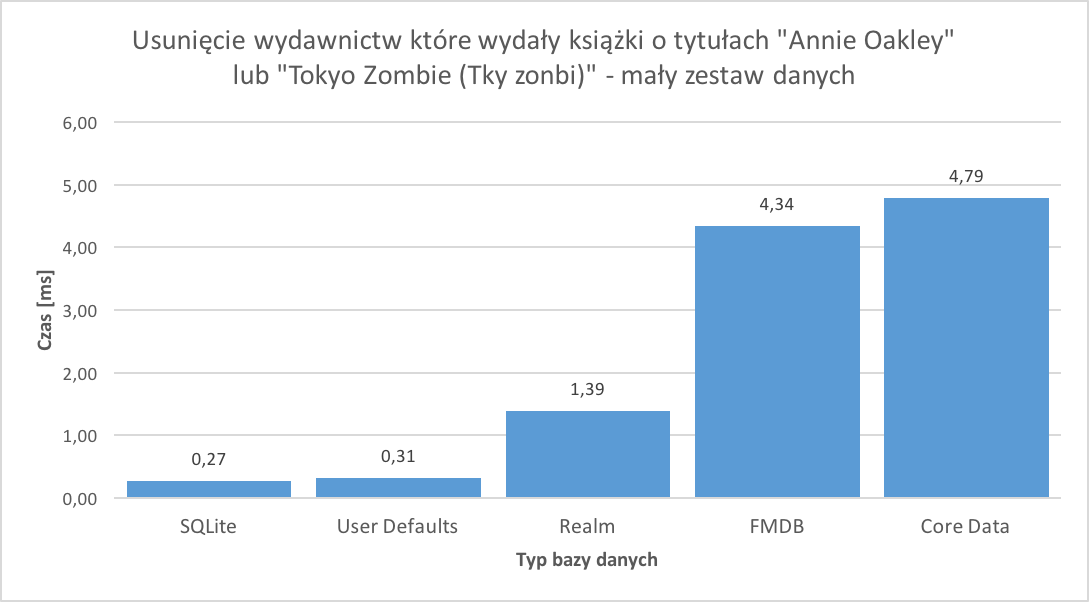
\includegraphics[width=\linewidth]{img/delete_data/delete_by_publisher/delete_by_publisher_small_test.png}
    \caption{Usunięcie wydawnictw, które wydały książki o~tytułach ,,Annie Oakley'' lub ,,Tokyo Zombie (Tky zonbi)'' - mały zestaw danych}
    \label{img: delete-by-publisher-small}
\end{figure}

\begin{figure}[H]
    \centering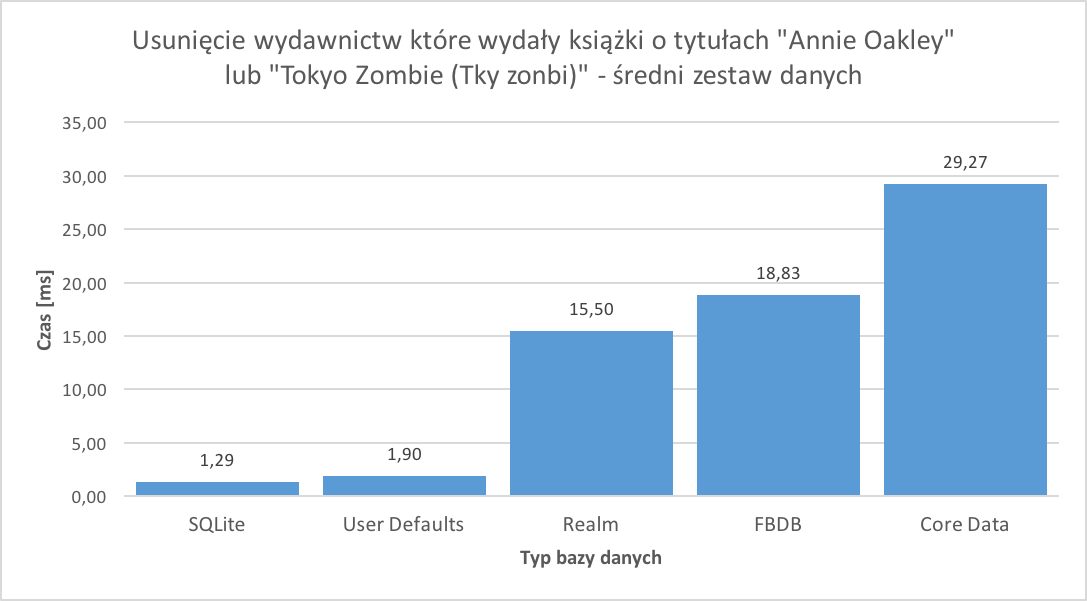
\includegraphics[width=\linewidth]{img/delete_data/delete_by_publisher/delete_by_publisher_medium_test.png}
    \caption{Usunięcie wydawnictw, które wydały książki o~tytułach ,,Annie Oakley'' lub ,,Tokyo Zombie (Tky zonbi)'' - średni zestaw danych}
    \label{img: delete-by-publisher-medium}
\end{figure}

\begin{figure}[H]
    \centering\includegraphics[width=\linewidth]{img/delete_data/delete_by_publisher/delete_by_publisher_big_test.png}
    \caption{Usunięcie wydawnictw, które wydały książki o~tytułach ,,Annie Oakley'' lub ,,Tokyo Zombie (Tky zonbi)'' - duży zestaw danych}
    \label{img: delete-by-publisher-big}
\end{figure}

Rezultaty testu usunięcia wydawnictw, które wydały książki o~tytułach ,,Annie Oakley'' lub ,,Tokyo Zombie (Tky zonbi)'' z~użyciem małego zestawu danych widoczne na wykresie \ref{img: delete-by-publisher-small} pokazują, że najszybszy w~tym przypadku okazał się SQLite. Uzyskał on czas równy 0.27 ms. Wolniej wykonała operacje Domyślna Baza Użytkownika kończąc zadanie w~ciągu 0.31 ms. Trzeci rezultat uzyskał Realm wykonując operacje w~1.39 ms. FMDB ukończył zadanie w~4.34 ms, zaś Core Data okazała się najwolniejsza czas zakończenia operacji, w~jej wykonaniu wyniósł 4.79 ms. 

 W~przypadku średniego zestawu danych ponownie najszybszy jest SQLite z~czasem 1.29 ms. Ponownie nieznacznie wolniejsza w~stosunku do SQLite okazała się Domyślna Baza Użytkownika, wykonując operacje w~1.90 ms. Realm przedstawia znaczny spadek wydajności względem poprzedników, kończąc zadanie po upływie 15.50 ms, co jest o~13.9 ms wolniej niż Domyślna Baza Użytkownika. FMDB i~Core Data ponownie okazały się najmniej wydajne. Czas wykonania testu dla FMDB wynosi 18.83 ms zaś dla Core Data równy jest on 29.27 ms.

Podczas wykorzystania dużego zestawu danych kolejność uzyskanych czasów przez bazy nie uległa zmianie. Ponownie najszybszy jest SQLite, czas wyniósł 6.63 ms. Znacznie wolniej operacje wykonała Domyślna Baza Użytkownika, zadanie wykonane zostało po upływie 24.92 ms. Realm zakończył operacje w~50.86 ms. FMDB zakończył usuwanie wybranych wydawnictwa w~czasie 94.44 ms. Core Data prezentuje znacznie wolniejsze działanie w~tego typu zapytaniach, uzyskała największy czas równy 174.6 ms. 

Test pokazuję, że w~przypadku operacji wymagającej pracy z~relacjami pomiędzy danymi, najszybszym rozwiązaniem jest SQLite. Domyślna Baza Użytkownika ponownie prezentuje duży spadek wydajności wraz ze wzrostem ilości danych. Realm i~FMDB prezentują zbliżone wyniki, lecz kiedy operacje wykonywane są na dużej ilości danych, zdecydowaną przewagę posiada Realm. Core Data, niezależnie od ilości danych, posiada najmniejszą wydajność spośród testowanych baz danych, niezależnie od ilości danych.

\subsection{Testy edycji danych}

Podrozdział przedstawia testy edycji danych w~dwóch różnych opcjach: 

\begin{itemize}
\item Zmiana imienia autora ,,Diena'' na ,,Alona''.
\item Zmiana daty wydania książek na obecna datę.
\end{itemize}

Pierwszy z~testów przedstawia operacje przeprowadzoną na wybranych rekordach z~tabeli, wymaga on przeszukania bazy w~celu odnalezienia odpowiedniego rekordu do edycji. Drugi test jest operacją przeprowadzaną na całej tablicy bez potrzeby wykonywania dodatkowych operacji wyszukiwania w~obrębie danego rekordu.

\subsubsection{Zmiana imienia autora ,,Diena'' na ,,Alona''}

\begin{figure}[H]
    \centering\includegraphics[width=\linewidth]{img/update_data/update_author/update_author_small_test.png}
    \caption{Zmiana imienia autora ,,Diena'' na ,,Alona'' - mały zestaw danych}
    \label{img: update-by-author-small}
\end{figure}

\begin{figure}[H]
    \centering\includegraphics[width=\linewidth]{img/update_data/update_author/update_author_medium_test.png}
    \caption{Zmiana imienia autora ,,Diena'' na ,,Alona'' - średni zestaw danych}
    \label{img: update-by-author-medium}
\end{figure}

\begin{figure}[H]
    \centering\includegraphics[width=\linewidth]{img/update_data/update_author/update_author_big_test.png}
    \caption{Zmiana imienia autora ,,Diena'' na ,,Alona'' - duży zestaw danych}
    \label{img: update-by-author-big}
\end{figure}

Test zmiany imienia autora ,,Diena'' na ,,Alona'' z~użyciem małego zestawu danych najszybciej wykonał SQLite, uzyskując czas 0.20 ms. Wraper FMDB zakończył to zadanie w~czasie 0.67 ms. Realm test zakończył po upływie 1.44 ms. Core Data pokazała niższa wydajność i~skończyła zadanie w~czasie 2.13 ms. Najwolniejsza okazała się Domyślna Baza Użytkownika, kończąc operacje w~czasie 2.31 ms. 

Zastosowanie średniego zestawu danych przyniosło następujące rezultaty. SQLite wykonał operacje w~czasie 0.45 ms. FMDB okazał się wolniejszy o~0.55 ms i~uzyskał czas 1 ms. Dla bazy Realm test zajął 1.47 ms. Core Data zakończyła zadanie w~czasie 2.73 ms. Ponownie najmniej wydajna jest Domyślna Baza Użytkownika, kończąc test w~3.43 ms.

Użycie dużego zestawu danych pokazuje, że SQLite w~dalszym ciągu jest bardzo wydajny, czas ukończenia operacji w~tym przypadku wyniósł 0.74 ms. Znacznie wolniejszy jest FMDB, zakończył test w~2.33 ms. Realm przy zwiększonej ilości danych uzyskał czas 2.66 ms, zaś Core Data potrzebowała 3.83 ms na edycje danych. Domyślna Baza Użytkownika po raz kolejny była najmniej wydajna, potrzebowała aż 4.36 ms, aby wykonać test. 

Test pokazuje, że wybranie odpowiednich rekordów i~ich edycja jest mocną stroną baz SQL, SQLite i~FMDB pokazują największą wydajność w~wykonanym teście niezależnie od ilości danych. Pozostałe bazy danych poddane testowi zwiększają swoje czasy wraz ze wzrostem ilości danych. Najmniej wydajną bazą w~przypadku przedstawionego testu jest Domyślna Baza Użytkownika. 

\subsubsection{Zmiana daty wydania książek na obecna datę}

\begin{figure}[H]
    \centering\includegraphics[width=\linewidth]{img/update_data/update_book/update_book_small_test.png}
    \caption{Zmiana daty wydania książek na obecna datę - mały zestaw danych}
    \label{img: update-by-book-small}
\end{figure}

\begin{figure}[H]
    \centering\includegraphics[width=\linewidth]{img/update_data/update_book/update_book_medium_test.png}
    \caption{Zmiana daty wydania książek na obecna datę - średni zestaw danych}
    \label{img: update-by-book-medium}
\end{figure}

\begin{figure}[H]
    \centering\includegraphics[width=\linewidth]{img/update_data/update_book/update_book_big_test.png}
    \caption{Zmiana daty wydania książek na obecna datę - duży zestaw danych}
    \label{img: update-by-book-big}
\end{figure}

Test zmiany daty wydania książek na obecna datę operował na wszystkich rekordach w~tabeli Książka. Rezultaty w~przypadku małego zestawu danych prezentują się następująco. Realm zakończył test w~czasie 0.74 ms. FMDB i~SQLite ukończyły operacje kolejno w~czasach 3.22 i~3.33 ms. Core Data okazała się znacznie wolniejsza od poprzedników i~potrzebowała 7.50 ms, aby zakończyć zadanie. Najwolniejsza jest Domyślna Baza Użytkownika, uzyskując czas wykonania operacji równy 10.15 ms. 

Średni zestaw danych w~przedstawianym teście przedstawia bardzo wysoką wydajność bazy Realm, zakończył on operacje w~2.49 ms. SQLite na wykonanie testu potrzebował 8.49 ms. FMDB zakończył zadanie w~czasie 17.58 ms. Znacznie wolniejsza od poprzednich baz jest Domyślna Baza Użytkownika, zakończyła test w~40.43 ms. Najwolniejsza jest Core Data, potrzebowała aż 172.88  ms na uaktualnienie dat wydania książek.

Użycie dużego zestawu danych pokazało, że w~dalszym ciągu Realm jest w~podanym teście najszybszy, czas zakończenia operacji wyniósł 8.57 ms. Dużo wolniejszy jest FMDB, potrzebował aż 75.59 ms. SQLite także potrzebował dużo czasu na zakończenie testu, operacja wymagała 136.73 ms. Domyślna Baza Użytkownika operacje zakończyła po upływie 306.18 ms. Core Data na wykonanie testu potrzebowała 490,68 ms. 

Podczas edycji każdego z~rekordów tabeli najwydajniejszą bazą okazał się Realm. Wolniejsze od dokumentowej bazy danych okazały się bazy SQL, edycja danych zajęła im więcej czasu. Najmniej wydajna jest Domyślna Baza Użytkownika oraz Core Data, której wydajność jest bardzo słaba w~przedstawionej operacji. 

\subsection{Podsumowanie wszystkich wyników}

Przeprowadzone testy dowodzą, że pod względem zużycia zasobów urządzenia, czyli pamięci operacyjnej i procesora bez względu na ilość danych, najlepsze okazują się bazy SQLite oraz FMDB. Stosunkowo najmniejszy plik wynikowy posiada Domyślna Baza Użytkownika i Realm. W sytuacji, kiedy potrzebna jest duża wydajność bazy danych podczas zapisu doskonałym rozwiązaniem okazuję się ponownie Realm i Domyślna Baza Użytkownika, niezależnie od ilości danych. Realm pokazuje wysoką wydajność podczas wykonywania operacji na średnich i dużych ilościach danych, lecz jego wydajność spada wraz ze wzrostem stopnia skomplikowania operacji. Bazy FMDB i SQLite są zaś wydajne przy skomplikowanych operacjach bazodanowych wykonywanych na większych ilościach danych. Core Data uzyskuje najlepsze wyniki podczas pracy nad średnią ilością danych. Domyślna Baza Użytkownika przystosowana jest do małej ilości danych oraz do wykonywania nieskomplikowanych zadań.

\section{Różnice implementacji baz danych}

 W~rozdziale zostały pokazane różnice i~podobieństwa w~implementacji poszczególnych rozwiązań bazodanowych. Przedstawiono fragmenty kodów wykonujące te same operacje przy użyciu różnych baz danych. Opisany też został stopień skomplikowania każdej z~operacji. 

\subsection{Modele danych}
Modele danych definiowane są różnie w~zależności od wykorzystanej bazy danych. W~przypadku Core Data używany jest edytor w~środowisku programistycznym XCode opisany w~drugim rozdziale pracy. Stworzony schemat bazy widoczny jest na rysunku \ref{fig: nosql_data_scheme}. Do poprawnego działania bazy Core Data wymagane jest wygenerowanie klas reprezentujących zaprojektowane tabele. Klasy te mogą zostać stworzone na kilka sposobów: ręcznie, za pomocą wbudowanego narzędzia w~XCode lub za pomocą dodatkowego programu typu ,,mogenerator". 

Bazy SQL przedstawione w~pracy używają standardowych poleceń SQL do stworzenia tabel i~relacji pomiędzy nimi. Przykład kodu źródłowego \ref{lis:create_SQL_table_code} prezentuje zapytania użyte w~stworzonym do testów  programie. 

\begin{code}[
		language=swift,
		caption={Polecenia tworzenia tabel w~SQLite i~FMDB},
		label={lis:create_SQL_table_code},
	]
    let createBookTableString = "CREATE TABLE IF NOT EXISTS Book (id INTEGER PRIMARY KEY AUTOINCREMENT, title TEXT, isbn TEXT, publishDate TEXT, publisher_id INTEGER, FOREIGN KEY(publisher_id) REFERENCES Publisher(id))"
    let createAuthorTableString = "CREATE TABLE IF NOT EXISTS Publisher (id INTEGER PRIMARY KEY AUTOINCREMENT, name TEXT)"
    let createPublisherTableString = "CREATE TABLE IF NOT EXISTS Publisher (id INTEGER PRIMARY KEY AUTOINCREMENT, name TEXT)"
\end{code}

 W~przypadku dokumentowej bazy Realm kolekcje tworzone są na podstawie obiektów dziedziczących z~klasy \textit{Object} biblioteki Realm. Kod źródłowy \ref{lis:realm_object_code} pokazuje przykład klasy.

\begin{code}[
		language=swift,
		caption={Przykład obiektu bazy Realm},
		label={lis:realm_object_code},
	]
class RAuthor: Object {
    
    @objc dynamic var id: Int = 0
    @objc dynamic var firstName = ""
    @objc dynamic var lastName = ""    
    var books = List<RBook>()
    
    override static func primaryKey() -> String? {
        return "id"
    }
}
\end{code}

 W~liniach 3-5 przedstawione są zmienne przechowujące dane obiektu, linia 6 pokazuje listę obiektów \textit{RBook}. Lista ta jest odwzorowaniem relacji pomiędzy tablicami. Metoda \textit{primaryKey()} znajdująca się w~linii numer 10 oznacza pole odpowiadające za klucz główny danej klasy. 

Domyślna Baza Użytkownika jak wspomniane zostało w~rozdziale 2.5 do konwersji obiektów wymaga rozszerzenia obiektów o~protokół \textit{NSCoding}. Przykład kodu klasy Domyślnej Bazy Użytkownika reprezentuje kod źródłowy \ref{lis:ud_object_code}. Tak jak w~w przypadku Realm linie 2-4 reprezentują pola przechowujące dane za w~linii 5 przedstawiona jest lista identyfikatorów książek wydanych przez danego autora. Lista ta reprezentuje relacje pomiędzy obiektami. Metoda \textit{encode(with aCoder: NSCoder)} potrzebna jest do poprawnego zapisu obiektu w~pamięci zaś funkcja \textit{convenience init(coder aDecoder: NSCoder)} odpowiada za odczyt obiektu.

\begin{code}[
		language=swift,
		caption={Przykład obiektu Domyślnej Bazy Użytkownika},
		label={lis:ud_object_code},
	]
class UDAuthor: NSObject, NSCoding {
    var authorId: Int
    var firstName: String
    var lastName: String
    var books: [Int]
    
    init(authorId: Int, firstName: String, lastName: String, books: [Int]) {
        self.authorId = authorId
        self.firstName = firstName
        self.lastName = lastName
        self.books = books
    }
    
    func encode(with aCoder: NSCoder) {
        aCoder.encode(authorId, forKey: "authorId")
        aCoder.encode(firstName, forKey: "firstName")
        aCoder.encode(lastName, forKey: "lastName")
        aCoder.encode(books, forKey: "books")
    }
    
    required convenience init(coder aDecoder: NSCoder) {
        let authorId = aDecoder.decodeInteger(forKey: "authorId")
        let firstName = aDecoder.decodeObject(forKey: "firstName") as! String
        let lastName = aDecoder.decodeObject(forKey: "lastName") as! String
        let books = aDecoder.decodeObject(forKey: "books") as! [Int]
        
        self.init(authorId: authorId, firstName: firstName, lastName: lastName, books: books)
    }
}

\end{code}

Można zauważyć znaczące różnice w~tworzeniu struktury danych w~każdej z~przedstawionych baz. Core Data dzięki dobremu wsparciu ze strony XCode może wydawać się prosta w~zaimplementowaniu lecz wymaga dobrej znajomosci całego framework-a. W~celu szybszej implementacji klas reprezentujących tabele trzeba skorzystać z~oddzielnych narzędzi co może przysporzyć dodatkowych problemów w~dalszych procesach utrzymywania oprogramowania. SQLite i~FMDB wymagają dobrej znajomości języka SQL, ale dobrze napisane polecenia są w~stanie posłużyć przez wiele lat gdyż język SQL jest jednym z~najstabilniejszych i~najpopularniejszych rozwiązań bazodanowych. Realm wymaga stosunkowo małej ilości kodu i~umiejętności aby stworzyć strukturę bazy. Klasy są bardzo przejrzyste i~zbliżone do zwykłych klas obiektów w~języku Swift. Domyślna Baza Użytkownika poza standardową deklaracją pól i~konstruktorów wymaga jeszcze zaimplementowania metod protokołu \textit{NSCoding}. Dodatkowo wymagane jest dodanie odpowiednich kluczy dla każdego z~pól obiektu. Ilość kodu i~kluczy uzależniona jest tutaj od ilości pól obiektu. Przy wielu tabelach może to stanowić znaczące problemy w~implementacji oraz utrzymaniu kodu. 

\subsection{Zapis danych}

Zapis danych w~przypadku Core Data przedstawiony jest w~przykładzie \ref{lis:core_data_save_code} znajdującym się poniżej.

\begin{code}[
		language=swift,
		caption={Przykład zapisu obiektu Core Data},
		label={lis:core_data_save_code},
	]
    private func insertPublishers(list: [Publisher]) {
        list.forEach { (publisher) in
            let publisherObject = CDWydawnictwo(context: stack.managedObjectContext)
            publisherObject.fill(publisher: publisher)
            guard let booksList = publisher.books else { return }
            booksList.forEach({ (bookId) in
                guard let book = featchBook(bookId: bookId) else { return }
                book.wydawnictwo = publisherObject
                publisherObject.ksiazki.adding(book)
            })
        }
        stack.saveContext()
    }
\end{code}

Dla każdego obiektu z~listy tworzony jest obiekt \textit{CDWydawnictwo} będący reprezentacją rekordu w~tabeli wydawnictwo. W~linii za pomocą funkcji \textit{fill} uzupełniane są pola obiektu. Następnie dla każdej książki wydanej przez wydawnictwo w~pętli pokazanej w~linii 8 odczytywany jest obiekt \textit{CDKsiazka} wcześniej już zapisany w~bazie. Po odczytaniu obiektu następuję ustawienie relacji książka - wydawnictwo co reprezentują linie 10 i~11 w~przedstawionym przykładzie. Po wykonaniu opisanych operacji w~linii numer 15 następuję zapis stanu bazy Core Data. 

Podczas użycia baz SQLIte i~FMDB aby zapisać obiekt do bazy należy w~pierwszej kolejności zdefiniować odpowiednie zapytania. Aby poprawnie wprowadzać dane do przedstawionej w~pracy bazie testowej zostały użyte zapytania SQL widoczne w~przykładzie \ref{lis:insert_sql_query}. 

\begin{code}[
		language=swift,
		caption={Zapytania SQL do wprowadzania danych},
		label={lis:insert_sql_query},
	]
    private let insertBookDataQueryString = "INSERT INTO Book (title, isbn, publishDate) VALUES (?, ?, ?)"
    private let insertAuthorDataQueryString = "INSERT INTO Author (firstName, lastName) VALUES (?, ?)"
    private let insertPublisherDataQueryString = "INSERT INTO Publisher (name) VALUES (?)"
    private let insertAuthorsBooksDataQueryString = "INSERT INTO authors_books (book_id, author_id) VALUES (?, ?)"
\end{code}

Kolejnym krokiem jest odpowiednie użycie przedstawionych powyżej zapytań oraz przypisanie odpowiednich pól obiektu do zapytania. Czynności te dla bazy SQLite zostały pokazane w~fragmencie kodu \ref{lis:sqlite_save_code}. Przykład pokazuję zapis obiektu \textit{Książka}. Aby zapisać obiekt niezbędna jest zmienna typu \textit{OpaquePointer} reprezentująca obiekt zapytania do bazy danych. Za pomocą funkcji widocznej w~4 linii \textit{sqlite3\_prepare\_v2} zapytanie z~formy ciągu znaków konwertowane jest na obiekt. Następnie w~liniach 8-11 za pomocą funkcji \textit{sqlite3\_bind\_text} pola obiektu \textit{Książka} przypisywane są do zapytania. W~linii 13 przy użyciu \textit{sqlite3\_step} następuję wykonanie zapytania i~zapis obiektu do tablicy. Funkcja \textit{sqlite3\_reset} czyści przypisane w~zapytaniu zmienne i~umożliwia ponowne załadowane nowych danych do zapytania. W~linii 20 przykładu następuję zapis stanu bazy danych przy użyciu \textit{sqlite3\_finalize}.

\begin{code}[
		language=swift,
		caption={Przykład zapisu obiektu SQLIte},
		label={lis:sqlite_save_code},
	]
    private func insertBooks(list: [Book]) {
        var insertDataStatement: OpaquePointer?
        
        if sqlite3_prepare_v2(db, insertBookDataQueryString, -1, &insertDataStatement, nil) != SQLITE_OK {
            print("error create database statement")
        }
        
        list.forEach { (book) in
            sqlite3_bind_text(insertDataStatement!, 1, (book.title as! NSString).utf8String, -1, nil)
            sqlite3_bind_text(insertDataStatement!, 2, (book.isbn as! NSString).utf8String, -1, nil)
            sqlite3_bind_text(insertDataStatement!, 3, (book.stringDate as NSString).utf8String, -1, nil)
            
            if sqlite3_step(insertDataStatement!) != SQLITE_DONE {
                print("Could not insert row into Book table")
            }
            
            sqlite3_reset(insertDataStatement!)
        }
        
        sqlite3_finalize(insertDataStatement)
    }
\end{code}

Przy użyciu biblioteki FMDB użycie SQLite jest znacznie łatwiejsze. Bliźniacza metoda do zapisu obiektów \textit{Książka} została przedstawiona w~przykładzie \ref{lis:fmdb_save_code}. Proces zapisu obiektu jest znacząco ułatwiony. W~linii 2 poprzez funkcje \textit{open()} otwierane jest połączenie z~bazą danych. Następnie w~pętli wykonywana jest operacja \textit{executeUpdate}, która przyjmuje jako parametr zapytanie do bazy i~listę pól obiektu. Po zapisaniu wszystkich obiektów do bazy w~linii numer 15 wywoływana jest funkcja \textit{close} służąca do zamknięcia połączenia z~bazą danych. 

\begin{code}[
		language=swift,
		caption={Przykład zapisu obiektu FMDB},
		label={lis:fmdb_save_code},
	]
    private func insertBooks(list: [UDBook]) {
        guard database.open() else {
            print("Unable to open database")
            return
        }
        
        list.forEach({ (book) in
            do {
                try! database.executeUpdate(insertBookDataQueryString, values: [book.title, book.isbn, book.stringDate])
            } catch {
                print("failed: error.localizedDescription")
            }
        })
        
        database.close()
    }
\end{code}

Jedną z~najprostszych implementacji zapisu danych posiada Domyślna Baza Użytkownika. Kod wykonujący to samo zadanie co przytoczone wcześniej przykłady reprezentuje fragment kodu \ref{lis:ud_save_code}. Dzięki implementacji protokołu \textit{NSCoding} możliwe jest szybkie kodowanie i~dekodowanie obiektów. W~celu uzyskania formatu danych pozwalającego na zapis w~Domyślnej bazie użytkownika użyta została metoda \textit{NSKeyedArchiver.archivedData} przekształcająca listę obiektów na typ \textit{Data} a~następnie dane zostały zapisane za pomocą funkcji \textit{userDefaults.set} a~w ostatniej linii za pomocą metody \textit{synchronize} zapisany został stan bazy. 

\begin{code}[
		language=swift,
		caption={Przykład zapisu obiektu User Defaults},
		label={lis:ud_save_code},
	]
    private func insertBooks(list: [UDBook]) {
        let encodedData = NSKeyedArchiver.archivedData(withRootObject: list)
        userDefaults.set(encodedData, forKey: booksKey)
        userDefaults.synchronize()
    }
\end{code}

Biblioteka Realm także posiada prosty interfejs zapisu danych. Metoda wykonująca to zadanie przedstawiona została poniżej w~przykładzie \ref{lis:realm_save_code}. Cała operacja sprowadza się do stworzenia bloku zapisu \textit{write} i~wywołaniu metody \textit{add} z~listą obiektów przeznaczoną do zapisu. 

\begin{code}[
		language=swift,
		caption={Przykład zapisu obiektu Realm},
		label={lis:realm_save_code},
	]
    private func insertBooks(list: [RBook]) {
        try! realm.write {
            realm.add(list)
        }
    }
\end{code}

Można zauważyć, że najmniej wymagający interfejs do zapisu danych posiada biblioteka Realm. Składa się on praktycznie z~dwóch metod. Bardzo prosty zapis danych posiada także Domyślna Baza Użytkownika lecz w~jej przypadku należy dodatkowo w~każdym obiekcie implementować protokół \textit{NSCoding}. Jedną z~bardziej wymagających bibliotek jest Core Data. Zapis danych wymaga tutaj większej ilości kodu a~także konwersji zapisywanego obiektu do obiektu reprezentującego tablice bazy. Należy też zadbać o~zapisywanie kontekstu bazy w~odpowiednich momentach. Najbardziej wymagające są bazy SQL. SQLite i~FMDB wymagają sformułowania odpowiednich zapytań SQL, dodatkowo w~przypadku SQLite implementacja wymaga pojedynczego przypisywania pól obiektu do stworzonego zapytania. Problem ten znika przy użyciu FMDB lecz w~większości przypadków to rozwiązanie pomimo ułatwień w~implementacji okazuję się działać znacznie wolniej od SQLite. 

\subsection{Odczyt danych}
Odczyt danych zostanie porównany na podstawie funkcji użytej podczas testu przedstawionego w~rozdziale 6.2 polegającego na wyszukaniu wszystkich autorów o~imieniu ,,Diena". 

Wybrany przykład funkcja dla Core Data został przedstawiony poniżej w~kodzie źródłowym \ref{lis:core_data_read_code}. Do odczytu danych należy zainicjalizować obiekt \textit{NSFetchRequest} z~odpowiednią nazwą tablicy na której przeprowadzona ma zostać operacja. Następnie tworzony jest \textit{NSPredicate}, który odpowiada za odpowiednie wyszukanie rezultatu zapytania, w~tym przypadku wybraniu autorów o~konkretnym imieniu. Po prawidłowej konfiguracji operacja jest wykonywana za pomocą funkcji \textit{executeFetchRequest}, która jako parametr przyjmuje \textit{NSFetchRequest} i~kontekst bazy danych.

\begin{code}[
		language=swift,
		caption={Przykład odczytu danych Core Data},
		label={lis:core_data_read_code},
	]
    func getAuthorsByName() {
        let name = "Diena"
        
        let request = NSFetchRequest<NSFetchRequestResult>(entityName: CDAuthor.entityName())
        let predicate = NSPredicate(format: "name == %@", name)
        
        request.predicate = predicate
        
        guard let result = stack.executeFetchRequest(request: request, inContext: stack.managedObjectContext) else { return }
    }
\end{code}

Inny sposób przeszukiwania danych oferuje Domyślna Baza Użytkownika. Funkcja wykonująca te same zadanie została przedstawiona w~przykładzie \ref{lis:ud_read_code}.

\begin{code}[
		language=swift,
		caption={Przykład odczytu danych User Defaults},
		label={lis:ud_read_code},
	]
    func getAuthorsByName() {
        let name = "Diena"
        var result = [UDAuthor]()
        
        if  let authorsData = userDefaults.data(forKey: authorsKey) {
            let authorsList = NSKeyedUnarchiver.unarchiveObject(with: authorsData) as! [UDAuthor]
            result = authorsList.filter { firstName == name }
        }
    }
\end{code}


 W~5 linii za pomocą zdefiniowanego klucza dla tabeli odczytywane są wszystkie dane dla tablicy Autor. Następnie w~linii numer 6 następuję konwersja surowego typu danych na obiekty. Kolejnym krokiem jest przeszukanie listy i~wybranie autorów o~podanym imieniu. 

Bazy SQL do odczytania danych wymagały zdefiniowana zapytania widocznego poniżej. Zapytanie te zostało użyte dla bazy SQLite i~FMDB.

\begin{code}[
		language=swift,
		caption={Zapytanie SQL do odczytu danych},
		label={lis:sql_read_query_code},
	]
let selectAuthorByNameQueryString = "SELECT id, firstName, lastName FROM Author a~WHERE a.firstName = ?"
\end{code}

 W~przypadku użycia SQLite odczyt danych przeprowadzony był poprzez poprzez funkcje widoczna w~fragmencie kodu \ref{lis:sqlite_read_code}

\begin{code}[
		language=swift,
		caption={Przykład odczytu danych SQLite},
		label={lis:sqlite_read_code},
	]
    func getAuthorsByName() {
        let name = "Diena"
        var result = [Author]()
        var stmtAuthors: OpaquePointer?
        
        if sqlite3_prepare(db, selectAuthorByNameQueryString, -1, &stmtAuthors, nil) != SQLITE_OK {
            let errmsg = String(cString: sqlite3_errmsg(db)!)
            print("error preparing insert: errmsg")
            return
        }
        
        sqlite3_bind_text(stmtAuthors!, 1, (name as! NSString).utf8String, -1, nil)
        
        while(sqlite3_step(stmtAuthors) == SQLITE_ROW) {
            let id = Int(sqlite3_column_int(stmtAuthors, 0))
            let firstName = String(cString: sqlite3_column_text(stmtAuthors, 1))
            let lastName = String(cString: sqlite3_column_text(stmtAuthors, 2))
            
            result.append(Author(authorId: id, firstName: firstName, lastName: lastName))
        }
    }
\end{code}

Ponownie w~przypadku SQLite wcześniej zdefiniowane zapytanie zostaje przypisane do obiektu typu \textit{OpaquePointer} za pomocą funkcji \textit{sqlite3\_prepare}. Następnie w~linii 12 do zapytania zostaje przypisany parametr oznaczony za pomocą "?" w~zapytaniu. W~linii numer 14 za pomocą funkcji \textit{sqlite3\_step} w~pętli odczytywane są kolejne rekordy będące wynikiem zapytania. Każde z~pól obiektu musi zostać odczytane i~sformatowane na odpowiedni typ. 

Operacja odczytu została ułatwia FMDB w~stosunku do SQLite. Funkcja wykonująca tą samą operacje przy użyciu bazy FMDB została przedstawiona poniżej. 

\begin{code}[
		language=swift,
		caption={Przykład odczytu danych FMDB},
		label={lis:fmdb_read_code},
	]
func getAuthorsByName() {
        let name = "Diena"
        var authorsList = [Author]()
        
        guard database.open() else {
            print("Unable to open database")
            return
        }
        
        do {
            let result = try database.executeQuery(selectAuthorByNameQueryString, values: [name])
            
            while(result.next()) {
                let id = Int(result.int(forColumnIndex: 0))
                let firstName = result.string(forColumnIndex: 1)
                let lastName = result.string(forColumnIndex: 2)
                
                authorsList.append(Author(authorId: id, firstName: firstName, lastName: lastName))
            }
        } catch {
            print("failed: (error.localizedDescription)")
        }
        
        database.close()
    }
\end{code}

FMDB po otworzeniu połączenia z~bazą umożliwia wykonanie zapytania za pomocą funkcji \textit{executeQuery} i~podaniu argumentów zapytania jako parametry funkcji. Następnie można iterować po kolejnych rekordach będących wynikiem zapytania. Rezultaty nie wymagają ponownego parsowania na odpowiednie typy. Po zakończeniu operacji należy pamiętać o~zamknięciu połączenia z~bazą danych za pomocą funkcji \textit{close}. 

Jedną z~najprostszych implementacji posiada biblioteka Realm. Przykład reprezentuje fragment kodu \ref{lis:realm_read_code}.

\begin{code}[
		language=swift,
		caption={Przykład odczytu danych Realm},
		label={lis:realm_read_code},
	]
    func getAuthorsByName() {
        let name = "Diena"
        let predicate = NSPredicate(format: "firstName = %@", name)
        let result = realm.objects(RAuthor.self).filter(predicate)
    }
\end{code}

Realm tak samo jak Core Data używa \textit{NSPredicate} do sformułowania zapytania odczytu danych. W~linii 4 za pomocą funkcji \textit{object()}, podając odniesienie do klasy, której rezultat chcemy otrzymać istnieje możliwość odczytania wszystkich rekordów. Następnie za pomocą funkcji \textit{filter}, której argumentem jest wcześniej zdefiniowany predykant następuje filtrowanie wyniku. 

Odczyt danych jest inny dla każdej z~bibliotek. Core Data pomimo dość prostej składni tworzenia zapytań posiada często problematyczne w~użyciu sformułowania predykantów. Domyślna Baza Użytkownika operuje jedynie na funkcjach filtrowania oferowanych przez środowisko przez co często operacje są znacznie wolniejsze niż w~przypadku innych rozwiązań bazodanowych. Dużym problemem jest też sytuacja kiedy wyszukanie rezultatu wymaga przeszukania relacji lub filtrowania wielu parametrów. W~takich przypadkach wymagane jest stworzenie wielu funkcji co niesie za sobą duży nakład kodu. SQLite posiada problematyczne przypisywanie argumentów do zapytania a~także wymaga parsowania odczytanych pól na odpowiednie typy. FMDB rozwiązuje te problemy lecz ilość kodu potrzebnego na zaimplementowanie jest zbliżona do implementacji SQLite. Jeden z~najprostszych sposobów implementacji posiada Realm. Odczytanie danych sprowadza się jedynie do kilku linii kodu. Oferuje on także możliwość używania predykatów tak samo jak w~przypadku Core Data a~także zwykłego filtrowania wyniku jak Domyślna Baza Użytkownika.


\subsection{Usuwanie danych}

Usuwanie danych zostanie porównane na podstawie funkcji użytej podczas testu przedstawionego w~rozdziale 6.3 polegającego na usunięciu wszystkich autorów, którzy wydali 3 książki.

 Kod źródłowy \ref{lis:core_data_delete_code} przedstawia przykład usuwania danych przy użyciu biblioteki Core Data. W~usuwaniu danych tak samo jak podczas odczytu tworzony jest \textit{NSFetchRequestResult} za pośrednictwem którego odczytywane są dane z~określonej tabeli. Następnie otrzymany rezultat jest filtrowany. Po przefiltrowaniu w~linii 9 wykonywana jest operacja usuwania wybranych rekordów. Standardowo po wszystkich operacjach następuje zapis stanu bazy danych.
 
\begin{code}[
		language=swift,
		caption={Przykład usuwania danych Core Data},
		label={lis:core_data_delete_code},
	]
    func removeAuthorsByBooks() {
        let requestAuthors = NSFetchRequest<NSFetchRequestResult>(entityName: CDAutor.entityName())
        
        guard var result = stack.executeFetchRequest(request: requestAuthors, inContext: stack.managedObjectContext) as? [CDAutor] else { return }
        result = result.filter { 0.ksiazki.count == 3 }
        
        result.forEach { (author) in
            stack.managedObjectContext.delete(author)
        }
        
        stack.saveContext()
    }
 \end{code}
    
Kod źródłowy \ref{lis:ud_delete_code} reprezentuje usuwanie danych w~Domyślnej Bazie Użytkownika. W~przykładzie widać słabe strony tego rozwiązania bazodanowego. W~linii 4 następuje filtrowanie listy zapisanych rekordów w~taki sposób aby wyszukać identyfikatory autorów których należy usunąć. W~linii 5 wykonywane jest ponowne przeszukanie listy rekordów i~usunięcie wybranych danych. W~przypadku złożonych operacji podczas używania Domyślnej Bazie Użytkownika często istnieje potrzeba przeszukiwania kilkukrotnie więcej niż jednej listy. Często jest to problematyczne w~zaimplementowaniu oraz znacząco spowalnia aplikacje.
    
\begin{code}[
		language=swift,
		caption={Przykład usuwania danych User Defaults},
		label={lis:ud_delete_code},
	]
        func removeAuthorsByBooks() {
        if  let authorsData = userDefaults.data(forKey: authorsKey) {
            let authorsList = NSKeyedUnarchiver.unarchiveObject(with: authorsData) as! [UDAuthor]
            let resultIdsToRemove = authorsList.filter { 0.books.count == 3 }.map { 0.authorId }
            let result = authorsList.filter { !resultIdsToRemove.contains(0.authorId) }
            let encodedData = NSKeyedArchiver.archivedData(withRootObject: result)
            userDefaults.set(encodedData, forKey: authorsKey)
            userDefaults.synchronize()
        }
    }
\end{code}

Bazy SQL do usuwania danych wymagały zdefiniowana zapytania widocznego poniżej. Zapytanie te zostało użyte dla bazy SQLite i~FMDB.

\begin{code}[
		language=swift,
		caption={Zapytanie SQL do usuwania danych},
		label={lis:sql_delete_query_code},
	]
let deleteAuthorsByBooks = "DELETE FROM Author WHERE EXISTS (SELECT authorId FROM ( SELECT Author.id as authorId, COUNT(authors_books.book_id) as booksCount FROM Author, authors_books WHERE Author.id = authors_books.author_id GROUP BY Author.id) WHERE booksCount = 3)"
\end{code}

Przykłady kodów źródłowych \ref{lis:sqlite_delete_code} (SQLite) i~\ref{lis:fmdb_delete_code} (FMDB) pokazują, że implementacja tego samego zadania nie różni się znacząco. Największą różnice pomiędzy nimi stanowi składnia. SQLite posiada składnie pokrewną dla języka C zaś biblioteka FMDB pomimo wykorzystywania SQLite udostępnia wszystkie funkcja charakterystyczne dla języka Swift. 

\begin{code}[
		language=swift,
		caption={Przykład usuwania danych SQLite},
		label={lis:sqlite_delete_code},
	]
    func removeAuthorsByBooks() {
        var stmtAuthors: OpaquePointer?
        
        if sqlite3_prepare(db, deleteAuthorsByBooks, -1, &stmtAuthors, nil) != SQLITE_OK {
            let errmsg = String(cString: sqlite3_errmsg(db)!)
            print("error preparing insert: (errmsg)")
            return
        }
        
        sqlite3_step(stmtAuthors!)
        sqlite3_finalize(stmtAuthors)
    }
\end{code}

\begin{code}[
		language=swift,
		caption={Przykład usuwania danych FMDB},
		label={lis:fmdb_delete_code},
	]
    func removeAuthorsByBooks() {
        guard database.open() else {
            print("Unable to open database")
            return
        }

        do {
            try database.executeStatements(deleteAuthorsByBooks)
        } catch {
            print("failed: (error.localizedDescription)")
        }
        
        database.close()
    }
\end{code}

Najmniej wymagający interfejs posługiwania się bazą danych zaprezentowany został w~przykładzie \ref{lis:realm_delete_code}. Biblioteka Realm wymaga jedynie przefiltrowania listy rekordów a~następnie przekazanie rezultatu jako argument funkcji \textit{delete}. 

\begin{code}[
		language=swift,
		caption={Przykład usuwania danych Realm},
		label={lis:realm_delete_code},
	]
    func removeAuthorsByBooks() {
        try! realm.write {
            let authors = realm.objects(RAuthor.self).filter { 0.books.count == 3 }
            realm.delete(authors)
        }
    }
\end{code}

Przykłady usuwania danych bardzo dobrze pokazują w~jakim stopniu różni się sposób implementacji operacji na danych w~przypadku różnych bibliotek. Core Data posiada swój charakterystyczny sposób przeprowadzania operacji za pomocą \textit{NSFetchRequest}. Implementacja SQLite i~FMDB są do siebie zbliżone. W~przypadku SQLite implementacja może wydawać się trudniejsza ze względu na interfejs C biblioteki. Domyślna Baza Użytkownika jest doskonałym rozwiązaniem do prostych operacji. Podczas skomplikowanych operacji na danych ilość kodu i~czas poświęcony na implementacje wzrasta. Najmniej wymagającą biblioteką jest dokumentowa baza Realm. Nie wymaga ona znaczących umiejętności od programisty a~także przeprowadzenie operacji na danych sprowadza się najczęściej do wywołania paru metod udostępnionych przez bibliotekę.

\section{Podsumowanie}

Celem pracy było porównanie wydajności oraz sposobów implementacji baz danych w~systemie iOS. Wykonane testy, przedstawione w~pracy pozwoliły porównać wydajność opisanych  baz danych. W~pracy przedstawione i~opisane zostały też fragmenty kodu dla każdej bazy danych potrzebne do wykonywania tych samych operacji. Przytoczone fragmenty kodu obrazują też różnice w~skomplikowaniu i~ilości potrzebnego kody do przeprowadzania tych samych zadań. 

Stworzono aplikacje na system iOS, która pozwala na wybranie bazy danych do testu, wykonanie odpowiednich testów, określenie ilości powtórzeń danego testu a~także wysłanie wyniku w~formacie CSV na adres email. 

Wykonano 10 różnych testów. Każdy z~testów został przeprowadzony na trzech zestawach danych: małym - 10-elementowym, średnim - 100-elementowym i~dużym - 1000-elementowym. Dodatkowo każdy z~testów dla uzyskania wiarygodnych wyników został wykonany sto razy. W~pracy testom zostały podane różne typy baz danych dlatego wynikiem końcowym każdego z~testów był moment otrzymania identycznych obiektów, które zostały uprzednio poddane zapisowi w~bazie. 

Podczas zapisu danych dominuje Domyślna Baza Użytkownika lecz należy pamiętać o~jej ograniczeniach takich jak brak relacji czy brak możliwości zapisu zdjęć. Baza Realm w~testach zapisu zajmuje drugie miejsce pod względem uzyskanych czasów, czas zapisu nie rośnie znacząco podczas zwiększania ilości zapisywanych danych. Core Data znacząco Zwiększa czas wraz ze wzrostem ilości danych. Najwolniejsze podczas zapisu danych okazały się bazy SQLite i~FMDB co pozwala stwierdzić, że zapis danych nie jest ich mocną stroną. 

Testy odczytu wszystkich danych pokazują, że zależnie od ilości danych testowane bazy osiągają różne czasy wykonania operacji. Realm pomimo przedostatniego rezultatu przy małej ilości rekordów zwiększa czas odczytu nieznacznie wraz z~ilością danych. Domyślna Baza Użytkownika radzi sobie dobrze jedynie z~małą ilością danych. Core Data osiąga najmniejszy czas podczas pracy ze średnim zestawem danych. Bazy SQLite i~FMDB osiągają najgorsze rezultaty ze wszystkich testowanych baz danych. 

Testy odczytu wybranych danych, które wymagały przeszukania zbioru jednoznacznie pokazują, że w~takich operacjach najlepiej spisuję się baza SQLite. FMDB wykorzystująca SQLite posiada większe czasy wykonywania operacji. Rezultaty Domyślnej Bazy Użytkownika zależne są od stopnia skomplikowania operacji, im bardziej złożona operacja tym czas wykonania zadania jest większy. Core Data i~Realm w~tego typu testach wypada różnie, wpływ na wyniki ma ilość danych i~stopień trudności operacji.

 W~testach usuwania wszystkich danych dominuje Domyślna Baza Użytkownika i~Realm. Core Data posiada trzeci co do wielkości czas usunięcia małej i~średniej ilości danych. Całkowite czyszczenie bazy najwięcej trwa w~przypadku SQLite i~FMDB.  Testy wymagające przeszukania bazy i~usunięciu jedynie wybranych elementów pokazują, że im bardziej skomplikowana jest operacja tym lepsze są bazy SQLite i~FMDB. W~przeciwnym wypadku Realm i~Domyślna Baza Użytkownika uzyskują lepsze rezultaty. Najwolniej tego typu operacje przeprowadzane są przez Core Data. 

Edycje danych najwolniej wykonuje Domyślna Baza Użytkownika i~Core Data. Doskonale zaś radzą sobie bazy SQL a~także Realm, który najlepiej spisuję się podczas edycji całych tabel. 

Przytoczone fragmenty kodu obrazują sposoby i~różnice implementacji użytych w~pracy baz danych. Najmniejszy nakład pracy programisty wymagany jest podczas używania bazy Realm. Dostarcza ona doskonały interfejs dzięki, któremu nawet skomplikowane operacje programista jest w~stanie zaimplementować za pomocą jedynie kilku linii kodu. Core Data wymaga doskonałej znajomości tego narzędzia, nakład kodu jest większy niż w~przypadku Realm. SQLite posiada nieczytelny interfejs a~także wymaga bardzo dobrej znajomości baz SQL. Operację są trudne w~zaimplementowaniu. Opisane problemy bazy SQLite eliminuje biblioteka opakowująca FMDB niestety wnosi ona opóźnienia przez, które wypada ona gorzej pod względem wydajności. Domyślna Baza Użytkownika wymaga jedynie znajomości języka programowania lecz implementacja skomplikowanych operacji jest bardzo skomplikowana i~wymaga dużej ilości kodu. 

Wskazanie najbardziej wydajnej bazy danych jest bardzo trudne. Uzależnione jest to od wielu czynników między innymi: ilości przechowywanych danych, rodzaju najczęściej wykonywanych operacji przez bazę czy też typu przechowywanych danych. Wydajność każdej z~bazy może też ulec zmianie poprzez wykorzystanie różnego typu dostępnych bibliotek do operacji na zmiennych. Tego typu biblioteki mogą znacząco poprawić wydajność baz SQL poprzez szybszą konwersje typów zmiennych przechowywanych w~obiektach programu pomiędzy typami wymaganymi do zapisu w~bazie. Jednoznacznie można zaś stwierdzić iż najprostszy interfejs i~sposób implementacji posiada biblioteka Realm.
%\section{Angular}
	15 września 2016 roku po blisko półtora roku prac Google wydało wzorowaną na poprzedniku, przepisaną od nowa nową wersję - Angular 2. Określana słowami \textit{One framework. Mobile \& desktop.} platforma programistyczna do tworzenia aplikacji internetowych na urządzenia mobilne i desktopowe z wykorzystaniem języka TypeScript. Implementuje podstawowe i opcjonalne funkcjonalności jako zbiór bibliotek gotowych do zaimportowania. W kolejnych podrozdziałach omówione zostaną podstawowe struktury i sposoby tworzenia aplikacji.
	
	\subsection{Nazewnictwo i wersjonowanie}  
	Początkowo Angular miał pozostać w wersji 2, tak samo jak AngularJS pozostał w wersji 1, dlatego właśnie początkowa nazwa - Angular 2 \cite{angular-versioning}. Jednak miesiąc po oficjalnej publikacji twórcy ogłosili zmianę sposobu wersjonowania na SEMVER (ang. \textit{Semantic Versioning}). Głównym celem SEMVER jest nadanie znaczenia numerom wersji. Pozwala to na zobrazowanie jak duże zmiany wprowadzono, a nawet umożliwienie narzędziom takim jak NPM (ang. \textit{Node Package Manager}) na aktualizowanie \blockquote{paczek} w automatyczny i bezpieczny sposób.\par
	
	Każda wersja składa się z 3 liczb. Przykładem jest \textit{2.5.3}. Kiedy naprawiony zostaje jakiś \textit{bug} zwiększana jest ostatnia liczba. Kiedy dodana jest nowa funkcjonalność zwiększana jest środkowa liczba. Kiedy wydanie posiada \textit{breaking change}, to znaczy zmianę taką, która zmusza użytkownika do dostosowania wcześniej działającego programu do nowej wersji, zwiększana jest pierwsza liczba.\par
	
	Dlatego właśnie początkowa nazwa Angular 2 od tamtej pory przekształciła się w Angular. Na czas pisania tej pracy najnowszą wersją jest 6.0.0.
	
	\subsection{RxJS}
	Jednym z założeń przepisania frameworku była zmiana sposobu detekcji zmian. Zdecydowano się na programowanie reaktywne. Jest to asynchroniczny paradygmat programowania dotyczący strumieni danych i propagacji zmian. Do tego celu użyto biblioteki RxJS (ang. \textit{Reactive Extensions for JavaScript}), która zapewnia implementację typu \textit{Observable} oraz dużą ilość operatorów (ponad 150), które umożliwiają dowolną manipulację strumieniami danych, ich łączenie, czy odwoływanie w czasie. W kodzie źródłowym \ref{lis:rxjs-example} przedstawiony został przykład wypisania na konsolę potęg liczb, które są mniejsze od 5.
	
	\begin{code}[
		language=javascript,
		caption={Przykład użycia RxJS (źródło: opracowanie własne)},
		label={lis:rxjs-example},
	]
Observable.of(1, 2, 3)
    .map(x => x * x)
    .filter(x => x < 5)
    .subscribe(x => console.log(x))
// Wynik:
// 1
// 4
	\end{code}	
	
	\subsection{TypeScript}
	Innym z założeń nowego frameworku, było to, aby był skalowalny. Bez względu na rozmiar aplikacji czytelność kodu nie powinna być skomplikowana. Jednym z takich problemów była trudność określenia typów zmiennych. W dużych programach bardzo łatwo popełnić błąd w nazwie pola obiektu lub pomylić jego typ, a ów problem uwidaczniał się dopiero w trakcie wykonania kodu. Z pomocą przyszedł, stworzony przez Microsoft, TypeScript \cite{typescript-doc}.\par
	
	TypeScript jest nadzbiorem JavaScript, to znaczy, że każdy poprawny program w JavaScript jest poprawnym programem w TypeScript, który pozwala na dodawanie statycznego typowania. Jest transpilowany do dowolnych wersji JavaScript, dzięki czemu funkcjonalności z najnowszych wersji ECMAScript nie są już przeszkodą w używaniu na starszych przeglądarkach.\par
	
	\begin{code}[
		language=javascript,
		caption={Przykład wykrycia błędu w TypeScript (źródło: opracowanie własne)},
		label={lis:typescript-example},
	]
function sayHello(name: string) {
  console.log("Hello " + name)
}

sayHello({ name: "John" })
	\end{code}		
	
	Przykład wykrycia błędu pokazano w kodzie źródłowym \ref{lis:typescript-example}. Funkcja \textit{sayHello} przyjmuje imię jako parametr i wita użytkownika komunikatem wyświetlonym w konsoli. Początkowo program wydaje się być poprawny, ale tak nie jest. Należy zwrócić uwagę na to, że funkcja przyjmuje nazwę jako \textit{string}, natomiast wywołana została z obiektem. W JavaScript problem zauważony zostałby dopiero po uruchomieniu programu. W przypadku TypeScript już sam kompilator zwraca błąd: \textit{error TS2345: Argument of type '{ name: string; }' is not assignable to parameter of type 'string'.} 
	
	\subsection{Kompilacja AOT}	
	Aplikacja Angularowa w większości składa się z komponentów i ich szablonów HTML. Przed wyrenderowaniem aplikacji przez przeglądarkę komponenty i szablony są tramspilowane przez kompilator Angulara do wykonywalnego kodu JavaScript. Angular oferuje 2 metody kompilacji: JIT (ang. \textit{Just-in-Time}) oraz AOT (ang. \textit{Ahead-of-Time}) \cite{angular-aot}.\par
	JIT, jak sama nazwa wskazuje, kompiluje aplikację dopiero w momencie uruchomienia w przeglądarce. Konsekwencją tego jest to, że oprócz samej aplikacji użytkownik musi pobrać również kompilator, który waży około 300kB. Może się to nie wydawać dużo, ale w erze urządzeń mobilnych każdy kilobajt się liczy. Oczywiście kompilowanie w trakcie wykonania posiada kolejny minus w postaci czasu. Im większy czas oczekiwania na interakcję z aplikacją, tym mniejsza ilość odwiedzających użytkowników, dlatego tak ważna jest jak najszybsza gotowość do użycia.\par
	AOT kompiluje aplikację już w trakcie budowania, a co za tym idzie użytkownik nie potrzebuje już pobierać kompilatora, przez co zaoszczędzi transfer danych i czas. Kolejnym plusem jest dołączenie szablonów HTML i arkuszów stylów CSS bezpośrednio do kodu JavaScript, dzięki czemu eliminuje się wysyłanie zapytań po te pliki. Kompilator AOT również wykrywa i zgłasza błędy wiązania szablonu HTML podczas kompilacji, zanim użytkownicy będą mogli je zobaczyć.
	
	\subsection{Podział na warstwy - NativeScript} \label{sec:angular-layers}
	AngularJS mógł być uruchomiony tylko w środowisku przeglądarki przez to, że był zależny od jQuery. Jednym z celów nowej wersji była możliwość uruchomienia aplikacji w różnych środowiskach. Dlatego zdecydowano się na podział na 2 warstwy \cite{angular-layers}: warstwę aplikacji oraz warstwę renderującą. Warstwa aplikacji zawiera API (ang. \textit{Application Programmin Interface}) oraz środowisko uruchomienia, z którym kod aplikacji komunikuje się bezpośrednio, a warstwa renderująca określa sposób, jak aktualizować UI (ang. \textit{User Interface}). Taka architektura warstwowa umożliwia działanie aplikacji na różnych platformach, tym samym nie zmieniając sposobu jej tworzenia. Aby stworzyć własną warstwę renderującą należy zaimplementować szereg interfejsów, w których struktury Angularowe tłumaczone są na język zrozumiały dla platformy, na której aplikacja miałaby zostać uruchomiona.\par
	NativeScript jest frameworkiem, który pozwala tworzyć natywne aplikacje mobilne używając Angulara, TypeScriptu lub JavaScriptu. Dzięki posiadaniu własnej warstwy renderującej, na podstawie kodu XML i komponentów renderuje elementy tak, jak miałoby to miejsce w przypadku kodu w Javie na Androida, lub w Swift na iOS.
	
	\subsection{Modularność}
	JavaScript i Angular używają modułów w celu organizacji struktury kodu i chociaż robią to w różny sposób, Angular używa obu tych technik.
	
	\subsubsection*{Moduły JavaScript}
	W JavaScript moduły to pojedyncze pliki z poprawnym kodem JavaScript. Aby sprawić, by pozostałe pliki mogły używać tego kodu wystarczy dopisać słowo kluczowe \textit{export} przed takimi strukturami, jak: funkcje, klasy, stałe, itp. Sposób ten przedstawiono w kodzie źródłowym \ref{lis:javascript-export-import} w linijce \ref{line:js-module-export}. Aby móc korzystać z kodu innych plików należy użyć schematu zaprezentowanego w linijce \ref{line:js-module-import}. Takie rozwiązanie zapobiega między innymi kolizji nazw oraz przypadkowym zmiennym globalnym.
	
	\begin{code}[
		language=javascript,
		caption={Stosowanie modułów JavaScript (źródło: \cite{javascript-module})},
		label={lis:javascript-export-import},
		escapechar=|
	]
// app.component.js
export class AppComponent { ... } |\label{line:js-module-export}|

// main.js
import { AppComponent } from './app.component'; |\label{line:js-module-import}|
	\end{code}	
	
	\subsubsection*{Moduły Angular}
	W Angular moduły są to klasy opisane dekoratorem \textit{@NgModule}. Zawierają on metadane na temat tego co dany moduł eksportuje, co importuje, jakie nowe struktury tworzy, od czego jest zależny, itp. W kodzie źródłowym \ref{lis:angular-module} przedstawiono deklarację modułu \textit{AppModule}, który deklaruje nowy komponent \textit{AppComponent} oraz importuje angularowy, zewnętrzny moduł przeglądarki \textit{BrowserModule}. Jak można zauważyć oba rodzaje modułów bardzo dobrze ze sobą współgrają.
	
	\begin{code}[
		language=javascript,
		caption={Stosowanie modułów Angular (źródło: \cite{javascript-module})},
		label={lis:angular-module},
		escapechar=|
	]
import { BrowserModule } from '@angular/platform-browser';
import { NgModule } from '@angular/core';
import { AppComponent } from './app.component';

@NgModule({
  declarations: [
    AppComponent
  ],
  imports: [
    BrowserModule
  ],
  providers: [],
  bootstrap: [AppComponent]
})
export class AppModule { }
	\end{code}\\
	
	Angular jako framework zawiera w sobie wiele gotowych do użycia modułów, których funkcjonalności przedstawiono w tabelce \ref{tab:angular-frequent-modules}.
	
	\begin{center}
    	\begin{table}[ht]
    	\begin{tabular}{ | l | l | p{5.5cm} |}
    \hline
    NgModule & Lokalizacja & Zastosowania \\ \hline
    BrowserModule & @angular/platform-browser & Kiedy aplikacja jest uruchamiana w przeglądarce \\ \hline
	CommonModule & @angular/common & Użycie dyrektyw takich jak: NgIf, NgFor, NgSwitch, NgClass, itp. \\ \hline
	FormsModule & @angular/forms & Podczas tworzenia formularzy opartych na szablonach \\ \hline
	ReactiveFormsModule & @angular/forms & Podczas tworzenia rektywnych formularzy \\ \hline
	RouterModule & @angular/router & Routing \\ \hline
	HttpClientModule & @angular/common/http & Wysyłanie zapytań HTTP typu AJAX \\ \hline
    \end{tabular}
    	\caption{Popularne moduły dołączone do Angular i ich zastosowania (źródło: \cite{angular-frequent-modules})}
    	\label{tab:angular-frequent-modules}
    	\end{table}
	\end{center}
	
	\subsection{Dołączanie danych}
	Domyślnie każde dołączenie danych jest jednokierunkowe, dzięki czemu maleje złożoność detekcji zmian. Zdecydowano się na podział na 3 sposoby:
	
	\subsubsection*{Jednokierunkowe ze źródła do celu}
	Stosowane przy dołączaniu do pól komponentu, dodawaniu dodatkowych atrybutów, takich jak \textit{aria-label}, dodawaniu klas, czy stylów lokalnych (ang. \textit{inline}). Składnię i przykładowe użycie przedstawiono w kodzie źródłowym \ref{lis:angular-one-way-binding-to-component}.
	
	\begin{code}[
		language=javascript,
		caption={Składnia i użycie dołączenia jednokierunkowego ze źródła do celu (źródło: \cite{angular-template-syntax})},
		label={lis:angular-one-way-binding-to-component},
		escapechar=|,
		keywords={},
	]
// Syntax
{{expression}}
[target]="expression"
bind-target="expression"

// Use
<img [src]="heroImageUrl">
<button [attr.aria-label]="help">help</button>
<div [class.special]="isSpecial">Special</div>
<button [style.color]="isSpecial ? 'red' : 'green'">
	\end{code}
	
	\subsubsection*{Jednokierunkowe od celu do źródła}
	Stosowane podczas reagowania na wydarzenia.	Jako wartość podaje się wyrażenie, które zostanie wywołane dopiero po jego zajściu. Dlatego istnieje bezpośrednia możliwość wywołania funkcji z odpowiednimi parametrami, zamiast przekazywania jej referencji. Składnię i przykładowe użycie przedstawiono w kodzie źródłowym \ref{lis:angular-one-way-binding-from-component}.
	
	\begin{code}[
		language=javascript,
		caption={Składnia i użycie dołączenia jednokierunkowego od celu do źródła (źródło: \cite{angular-template-syntax})},
		label={lis:angular-one-way-binding-from-component},
		escapechar=|,
		keywords={},
	]
// Syntax
(target)="statement"
on-target="statement"

// Use
<button (click)="onSave()">Save</button>
<div (myClick)="clicked=\$event" clickable>click me</div>
	\end{code}
	
	\subsubsection*{Dwukierunkowe}
	Stosowane, gdy istnieje potrzeba wyświetlenia i aktualizowania danych, gdy użytkownik przeprowadzi zmiany. Najczęstszą sytuacją jest dołączenie wartości do elementu HTML \textit{<input/>}, której aktualna wartość powinna być pokazana w polu tekstowym, a jej zmiana powinna być odzwierciedlona w stanie aplikacji. Składnię i przykładowe użycie przedstawiono w kodzie źródłowym \ref{lis:angular-two-way-binding}.
	
	\begin{code}[
		language=javascript,
		caption={Składnia i użycie dołączenia dwukierunkowego (źródło: \cite{angular-template-syntax})},
		label={lis:angular-two-way-binding},
		escapechar=|,
		keywords={},
	]
// Syntax
[(target)]="expression"
bindon-target="expression"

// Use
<input [(ngModel)]="name">
	\end{code}
	
	\subsection{Komponenty}
	Tak jak w AngularJS pozostano przy koncepcji komponentów i dyrektyw. Jednak w tym przypadku to komponenty zostały głównymi strukturami zapewniającymi reużywalność powtarzających się części kodu. Tworzenie komponentów odbywa się za pomocą dekorowania klas dekoratorem \textit{@Component} lub dla dyrektywy \textit{@Directive}. Jako medatadane można przekazać, na przykład: listę animacji komponentu, nazwę selektora, atrybuty wychodzące, sposób detekcji zmian i wiele innych. W kodzie źródłowym \ref{lis:angular-component} przedstawiony został komponent oferujący taką funkcjonalność, jak dyrektywa pokazana w podrozdziale \ref{page:angularjs-directives-and-components} \textit{Dyrektywy i komponenty}.
	
	\begin{code}[
		language=javascript,
		caption={Użycie komponentu w Angularze (źródło: opracowanie własne)},
		label={lis:angular-component},
		escapechar=|
	]
// customer.ts
@Component({
  selector: 'my-customer',
  template: `Name: {{customer.name}}, Address: {{customer.address}}`
})
export class CustomerComponent {
  customer = {
    name: 'Adam',
    address: 'Belveder st.'
  }
}
  
// app.html
<my-customer></my-customer> <!-- Name: Adam, Address: Belveder st. -->
	\end{code}
	
	\subsubsection{Dane wejściowe i wyjściowe}
	Jednak komponent powinien być elastyczny i pozwalać na ponowne użycie za pomocą danych wejściowych i wyjściowych. W tym celu ponownie zastosowano metodę dekorowania, w tym wypadku pól klas komponentów lub dyrektyw, dekoratorami \textit{@Input} i \textit{@Output}. W kodzie źródłowym \ref{lis:angular-component-input-output-create} pokazany został przykład tego samego komponentu przyjmującego obiekt klienta jako dane wejściowe (linijka \ref{line:angular-input}) oraz emitującego dane wyjściowe (linijka \ref{line:angular-output-use}). W tym wypadku jest to napis emitowany co 1 sekundę.\par
	W kodzie źródłowym \ref{lis:angular-component-input-output-use} przedstawione zostało użycie  komponentu \textit{CustomerComponent} jako elementu HTML (linijka \ref{line:angular-component-element}). Warto zwrócić uwagę na sposób przekazywania danych jako atrybuty. W atrybucie \textit{[customer]} nawiasy klamrowe informują kompilator, że dane mają zostać dołączone jednokierunkowo do komponentu do polu o tej samej nazwie. W atrybucie \textit{(helloEmitter)} nawiasy klamrowe informują kompilator, że funkcja \textit{greet} powinna być wywołana za każdym razem kiedy nastąpi emisja danych, a jej parametrem ma być ta emitowana wiadomość. Takie oddzielenie składni pozwala na łatwe dostrzeżenie danych wchodzących, jak i wychodzących.

	\begin{code}[
		language=javascript,
		caption={Utworzenie komponentu z danymi wejściowymi Angularze (źródło: opracowanie własne)},
		label={lis:angular-component-input-output-create},
		escapechar=|
	]
// customer.ts
export interface User {
  name: string;
  address: string;
}
@Component({
  selector: 'my-customer',
  template: `Name: {{customer.name}}, Address: {{customer.address}}`
})
export class CustomerComponent implements OnInit, OnDestroy {
  @Input() customer: User; |\label{line:angular-input}|
  @Output() helloEmitter = new EventEmitter<string>();
  private intervalId;

  ngOnInit(): void { |\label{line:angular-ngOnInit}|
    this.intervalId = setInterval(() => {
      this.helloEmitter.emit('Hello: ' + this.customer.name); |\label{line:angular-output-use}|
    }, 1000);
  }
  ngOnDestroy(): void { |\label{line:angular-ngOnDestroy}|
    clearInterval(this.intervalId);
  }
}
	\end{code}
	
	\begin{code}[
		language=javascript,
		caption={Użycie komponentu z danymi wejściowymi Angularze (źródło: opracowanie własne)},
		label={lis:angular-component-input-output-use},
		escapechar=|
	]
// app.ts
@Component({
  selector: 'app-root',
  template: `
<my-customer |\label{line:angular-component-element}|
  [customer]="myCustomer"
  (helloEmitter)="greet(\$event)"
></my-customer> 
  `
})
export class AppComponent {
  myCustomer: User = {
    name: 'Adam',
    address: 'Belveder st.'
  };
  greet(message: string) {
    console.log(message);
  }
}
	\end{code}
	
	\subsubsection{Cykl życia}
	Każdy komponent ma własny cykl życia zarządzany przez framework \cite{angular-lifecycle-hooks}. Angular tworzy komponent, renderuje go, tworzy i renderuje jego dzieci, sprawdza zamianę danych wejściowych i niszczy go przed usunięciem z drzewa DOM. Istnieje możliwość implementacji  jednej lub wielu funkcji wywoływanych właśnie w tych kluczowych momentach. Tak samo zachowują się również dyrektywy.\par
	Przykład użycia zaprezentowano w kodzie źródłowym \ref{lis:angular-component-input-output-create} w linijkach \ref{line:angular-ngOnInit} i \ref{line:angular-ngOnDestroy}. W metodzie \textit{ngOnInit()}, która wywoływana jest tuż po utworzeniu komponentu, uruchomiony zostaje licznik emitujący co sekundę napis. W metodzie \textit{ngOnDestroy()}, która wywoływana jest tuż przed usunięciem komponentu licznik ten zostaje zatrzymany w celu uniknięcia wycieków pamięci.
	
	\subsection{Dyrektywy}
	W Angularze istnieją 2 rodzaje dyrektyw: atrybutowe i strukturalne. Używa się ich za pomocą atrybutów elementów HTML. Atrybutowe \cite{angular-attribute-directives} zmieniają wygląd lub zachowanie elementu drzewa DOM.  Natomiast strukturalne \cite{angular-structural-directives} manipulują drzewem DOM.\par
	Angular posiada moduł z kilkoma bardzo przydatnymi dyrektywami strukturalnymi. W kodzie źródłowym \ref{lis:angular-structural-directives} w linijce \ref{line:angular-ngif} użyta została dyrektywa \textit{ngIf}, która usuwa z drzewa DOM element, na którym została użyta, jeśli wyrażenie użyte jako jej wartość jest fałszywe. W linijce \ref{line:angular-ngfor} użyta zostałą dyrektywa \textit{ngFor}, która powiela element, na którym została użyta, tyle razy, ile istnieje elementów w tablicy \textit{customers}. Składnia wyrażenia przypomina tą z pętli \textit{for/of} w ECMAScript 6. Warto zauważyć, że użycie dyrektyw strukturalnych jako atrybutów poprzedzone jest gwiazdką (\textit{*}).
	
	\begin{code}[
		language=javascript,
		caption={Użycie wbudowanych dyrektyw strukturalnych w Angularze (źródło: opracowanie własne)},
		label={lis:angular-structural-directives},
		escapechar=|
	]
<div *ngIf="age >= 18"> |\label{line:angular-ngif}|
  Adult
</div>

<div *ngFor="let c of customers"> |\label{line:angular-ngfor}|
  {{c.name}}
</div>
	\end{code}
	
	\subsection{Filtry}
	Zdecydowano się również na zachowanie Filtrów, choć teraz pod nazwą \textit{Pipes}. Ich rola pozostała niezmienna, lecz zmienił się tylko sposób ich tworzenia, tak jak pokazano to w kodzie źródłowym \ref{lis:angular-filter}.
	
	\begin{code}[
		language=javascript,
		caption={Utworzenie i użycie filtru w Angularze (źródło: opracowanie własne)},
		label={lis:angular-filter}
	]
// incrementer.pipe.ts
@Pipe({
  name: 'incrementer'
})
export class IncrementerPipe implements PipeTransform {
  transform(value: any, ...args: any[]): any {
    return value + 1;
  }
}

// app.html
<div>
	<p>{{5 | incrementer}}</p> <!-- 6 -->
</div>
	\end{code} 

	\subsection{Serwisy i wstrzykiwanie zależności}
	Tak jak AngularJS zdecydowano się na zastosowanie wstrzykiwania zależności. Dostarczenie zależności odbywa się poprzez przekazanie ich jako parametry konstruktora. Dlatego właśnie podczas deklaracji komponentów w modułach przekazuje się ich referencje, a nie utworzone już obiekty. Angular sam znajdzie i zdecyduje które obiekty użyć, a w przypadku ich braku wyrzuci odpowiedni wyjątek.\par
	Wstrzyknięcie odpowiednich obiektów można zawdzięczyć TypeScriptowi. Tak jak pokazano to w kodzie źródłowym \ref{lis:angular-serwis} przy parametrach konstruktora należy podać typ oczekiwanej wartości. Następnie za pomocą refleksji Angular jest w stanie wykryć jakie obiekty i w jakiej kolejności są potrzebne. Oczywiście istnieje możliwość zależności cyklicznej, czyli takiej, w której komponenty, czy serwisy są zależne od siebie nawzajem. W takim wypadku wstrzyknięcie zależności powinno odbyć się poprzez wstrzyknięcie serwisu \textit{Injector} a następnie wywołaniu na nim metody \textit{get()} z typem zależności cyklicznej.\par
	Podobnie jak w AngularJS zastosowano koncepcję serwisów. Każda klasa serwisu musi zostać opisana dekoratorem \textit{@Injectable()} a następnie jej referencja przekazana do modułu w tablicy \textit{providers}. Po tych krokach serwis dostępny jest do wykorzystania pozostałym strukturom tego modułu. W kodzie źródłowym \ref{lis:angular-serwis} przedstawiono zachowanie takie jak w kodzie źródłowym \ref{lis:angularjs-serwis}. 
	
	\begin{code}[
		language=javascript,
		caption={Utworzenie i użycie serwisu w Angularze (źródło: opracowanie własne)},
		label={lis:angular-serwis},
		escapechar=|
	]
@Injectable()
export class DateService {
  getCurrentDate(): Date {
    return new Date();
  }
}
@Component({selector: 'my-component', template: ''})
export class MyComponent implements OnInit {
  constructor(public dateService: DateService) {
  }
  ngOnInit(): void {
    console.log(this.dateService.getCurrentDate());
  }
}
@NgModule({
  providers: [DateService],
  declarations: [MyComponent]
})
export class MyModule {
}
	\end{code} 
	
	\subsection{Router}
	Angular posiada również moduł odpowiedzialny za płynne nawigowanie między widokami. W kodzie źródłowym \ref{lis:angular-router} przedstawiona została konfiguracja routera identyczna w stosunku do tej z kodu źródłowego \ref{lis:angularjs-router}. Obiekt konfiguracyjny należy przekazać do statycznej metody \textit{forRoot} w trakcie importowania modułu do aplikacji.
	
	\begin{code}[
		language=javascript,
		caption={Konfiguracja routera w Angularze (źródło: opracowanie własne)},
		label={lis:angular-router},
		escapechar=|
	]
const appRoutes: Routes = [
  {path: '/shop', component: ShopComponent},
  {path: '/shop/item/:itemId', component: ShopItemComponent},
];

@NgModule({
  imports: [
    RouterModule.forRoot(
      appRoutes,
    )
  ],
})
export class AppModule {
}
	\end{code} 
	


























 \label{angular-section}

%\section{ReactJS}
	 ReactJS jest to JavaScriptowa biblioteka do budowania interfejsów użytkownika wydana w 2013 roku przez firmę Facebook. Należy zwrócić uwagę, że twórcy określają ją jako bibliotekę, a nie framework, ponieważ jej jedyną funkcjonalnością jest tworzenie UI. Jednak przez framework można rozumieć szkielet do budowy aplikacji, który definiuje jej strukturę oraz ogólny mechanizm działania. ReactJS wpisuje się w tę definicję, dlatego w tej pracy postrzegany będzie właśnie jako framework. W kolejnych podrozdziałach, w przypadku braku funkcjonalności w samym ReactJS, omówione zostaną najpopularniejsze moduły tworzone przez społeczność w ramach oprogramowania o otwartym źródle.
	 
	 \subsection{JSX}
	 JSX (ang. \textit{JavaScript extension}) jest językiem rozszerzającym składnię JavaScript. Najważniejszą jego funkcjonalnością jest możliwość bezpośredniego używania znaczników HTML w kodzie JavaScript. Takiego formatu nie obsługuje żadna przeglądarka, dlatego niezbędnym krokiem jest przekształcenie go do JavaScriptu. W kodzie źródłowym \ref{lis:reactjs-jsx} przedstawiony został przykład, gdzie funkcja \textit{getElement} zwraca element \textit{MyButton} przed i po transpilacji. Warto zwrócić uwagę, że wartości atrybutów mogą być ustawiane dynamicznie, dzięki zamianie cudzysłowów na nawiasy klamrowe (linijka \ref{line:jsx-attrs}).
	  
	 \begin{code}[
		language=javascript,
		caption={Przykład użycia JSX (źródło: \cite{reactjs-jsx})},
		label={lis:reactjs-jsx},
		escapechar=|
	]
// Przed
const getElement = size => (
  <MyButton color="blue" shadowSize={size}> |\label{line:jsx-attrs}|
    Click Me
  </MyButton>)
// Po
const getElement = size => (
  React.createElement(
    MyButton,
    { color: 'blue', shadowSize: size },
    'Click Me'
  ))
	\end{code}
	
	 \subsection{Redux}
	 ReactJS nie posiada mechanizmu do globalnego przechowywania stanu aplikacji. W związku z tym najczęściej wybieraną do tego biblioteką jest Redux. Jej cechami są: proste API, przewidywalność i łatwość w testowaniu.\par
	 Główną ideą jest przechowywanie stanu całej aplikacji w jednym obiekcie, tzw. \textit{store}. Jedynym sposobem na zmianę którejkolwiek z wartości jest wysłanie akcji, czyli obiektu opisującego co się wydarzyło. Aby określić w jaki sposób akcje przekształcają drzewo stanu należy utworzyć reduktory, czyli czyste funkcje, które na podstawie tych samych danych wyjściowych zwrócą zawsze ten sam wynik.
	 
	 \begin{code}[
		language=javascript,
		caption={Przykład użycia Redux (źródło: opracowanie własne)},
		label={lis:reactjs-redux},
		escapechar=|
	]
// Store
const initialState = { |\label{line:redux-store}|
  name: 'John',
  age: 15
}
// Reducer
function reducer(state = initialState, action) { |\label{line:redux-reducer}|
  switch (action.type) {
    case 'MULTIPLY_AGE_BY':
      return {
        ...state,
        age: state.age * action.payload
      }
    default:
      return state
  }
}
// Action
const action = { |\label{line:redux-action}|
  type: 'MULTIPLY_AGE_BY',
  payload: 2
}
dispatch(action)

	\end{code}\\
	
	W kodzie źródłowym \ref{lis:reactjs-redux} przedstawiony został przykład wykorzystania  koncepcji oferowanej przez Redux. W linijce \ref{line:redux-store} tworzony jest obiekt \textit{store}, z początkowymi wartościami, przechowujący stan aplikacji. W linijce \ref{line:redux-reducer} tworzony jest reduktor, który na podstawie stanu i akcji definiuje nowy stan. W linijce \ref{line:redux-action} jest tworzona i wysyłana akcja. Całym procesem zarządza Redux.
	 
	 \subsection{Komponenty}
	 Głównymi elementami, z których na składa się ReactJS są, tak jak w Angularze, komponenty. Dzielą UI na niezależne, reużywalne części. Każdy komponent posiada metodę \textit{render()}, która zwraca to, jak powinien wyglądać. Stan komponentu przechowywany jest w polu \textit{state}, którego aktualizacja powinna odbywać się za pomocą metody \textit{setState({...})}, po wywołaniu której ReactJS \blockquote{wie}, kiedy zaktualizować widok, czyli wywołać metodę \textit{render()}. W kodzie źródłowym \ref{lis:reactjs-component-create} przedstawiony został komponent reprezentujący funkcjonalność identyczną, jak w przypadku Angulara (kod źródłowy \ref{lis:angular-component-input-output-create}).
	 
	 \subsubsection{Dane wejściowe i wyjściowe}  
	 W ReactJS istnieje możliwość przekazywania wartości do komponentu. poprzez właściwości (ang. \textit{props}). Dane te są dostępne w komponencie w polu o nazwie \textit{props} tak, jak zrobiono to w kodzie źródłowym \ref{lis:reactjs-component-create} w linijce \ref{reactjs-props-use}. Jako parametr została przekazana funkcja \textit{helloEmitter}, która będzie wywoływana co 1 sekundę z odpowiednim parametrem. Należy mieć na uwadze, że tak dostępne właściwości są tylko do odczytu, to znaczy, że modyfikować je może tylko komponent przekazujący właściwości.
	 
	 \subsubsection{Cykl życia}
	 Tak, jak Angularze, w ReactJS istnieją również funkcje wywoływane przez framework w kluczowych momentach życia komponentu \cite{reactjs-component-doc}. Przykład użycia zaprezentowano w kodzie źródłowym \ref{lis:reactjs-component-create}, gdzie metoda \textit{componentDidMount()} wykonywana jest zaraz po utworzeniu komponentu, w której do stanu komponentu zapisywany jest identyfikator funkcji emitującej co sekundę wydarzenie. W metodzie \textit{componentWillUnmount()}, która wywoływana jest tuż przez usunięciem komponentu przeprowadzane jest czyszczenie wszystkich liczników, które powodowałyby wycieki pamięci.
	 
	 \begin{code}[
		language=javascript,
		caption={Utworzenie komponentu z danymi wejściowymi w ReactJS (źródło: opracowanie własne)},
		label={lis:reactjs-component-create},
		escapechar=|
	]
export class MyCustomer extends React.Component {
  componentDidMount() {
    this.setState({
      intervalId: setInterval(() => {
        this.props.helloEmitter('Hello: ' + this.customer.name) |\label{reactjs-props-use}|
      }, 1000)
    })
  }
  componentWillUnmount() {
    clearInterval(this.state.intervalId)
  }
  render() {
    return (
      <span>
        Name: {this.props.customer.name},
        Address: {this.props.customer.address}
      </span>
    )
  }
}
	\end{code}
	
	 \begin{code}[
		language=javascript,
		caption={Użycie komponentu z danymi wejściowymi w ReactJS (źródło: opracowanie własne)},
		label={lis:reactjs-component-use},
		escapechar=|
	]
export class App extends React.Component {
  state = {
    myCustomer: {
      name: 'Adam',
      address: 'Belveder st.'
    }
  }
  constructor(props) {
    super(props)
    this.greet = ::this.greet
  }
  greet(message) {
    console.log(message);
  }
  render() {
    return (
      <MyCustomer 
          customer={this.state.myCustomer}
          helloEmitter={this.greet}
      />
    )
  }
}
	\end{code}
	 
	 \subsection{React-Native}
	 React-Native jest frameworkiem, który przejmuje rolę renderowania komponentów natywnie na urządzeniach mobilnych. Nie renderuje tego we wbudowanym \textit{web-view}, który tylko próbuje naśladować natywne elementy, ale właśnie za pomocą tych natywnych na platformy, na której się wykonuje, czyli Android lub iOS. Dzięki takiemu zabiegowi aplikacja staje się bardziej wydajna, a proces tworzenia się prawie nie zmienia.
	 \subsection{Router}
	 ReactJS nie posiada wbudowanej nawigacji między widokami, dlatego aplikacje muszą korzystać z zewnętrznych pluginów. Najpopularniejszym z nich jest React-Router \cite{reactjs-router}. Konfiguracja polega na użyciu komponentu \textit{Route} z parametrem \textit{path}, określającym ścieżkę URL oraz \textit{componentent}, definiującym, który komponent powinien zostać wyrenderowany w przypadku pasującej ścieżki URL.
	 
	 \begin{code}[
		language=javascript,
		caption={Konfiguracja Routera w ReactJS (źródło: opracowanie własne)},
		label={lis:reactjs-router},
		escapechar=|
	]
const RouterConfig = () => (
  <Router>
    <Route path="/shop" component={ShopComponent} />
    <Route path="/shop/item/:itemId" component={ShotItemComponent} />
  </Router>
)
	\end{code}

%\section{VueJS}
	VueJS jest wieloplatformowym frameworkiem JavaScriptowym, którego pierwsza wersja pojawiła się w Lutym 2014 roku. Zapoczątkowany przez Evana You, byłego pracownika Google, który podczas wieloletniej pracy używał AngularJS w wielu projektach. Spodobały mu się w nim pewne koncepcje, które zdecydował przenieść do własnego frameworku. Celem była prostota, mały rozmiar, brak nie potrzebnych mechanizmów i zawiłości.

	\subsection{Komponenty}
	W VueJS również zastosowano koncepcję komponentów, jako reużywalnych części, z których składa się aplikacja. W kodzie źródłowym \ref{lis:vuejs-component-create} zostało przedstawione utworzenie komponentu o takich samych funkcjonalnościach, jak w kodzie źródłowym \ref{lis:angular-component-input-output-create} i \ref{lis:reactjs-component-create}. Przyjmuje on 2 parametry: \textit{customer}, którego wartości wyświetlane są w szablone i \textit{helloEmitter}, który wywoływany jest co sekundę. W kodzie źródłowym \ref{lis:vuejs-component-use} przedstawione zostało użycie tego komponentu i przekazanie w parametrach obiektu \textit{myCustomer} i funkcji \textit{greet()}. Taką samą funkcjonalność przedstawiono w kodzie źródłowym \ref{lis:angular-component-input-output-use} i \ref{lis:reactjs-component-use}\par
	W VueJS istnieją 2 typy komponentów: lokalne i globalne. Globalne nie potrzebują dodatkowego importowania z plików, ale przez to są podatne na kolizję w nazewnictwie. Tworzone są za pomocą \textit{Vue.component('my-customer',\{...\})}, gdzie pierwszy parametr, to nazwa komponentu, a drugi to obiekt konfiguracyjny. Tworzenie lokalnych komponentów różni się tylko nieznacznie. W oddzielnym pliku powinien znajdować się tylko jeden komponent, którego obiekt konfiguracyjny powinien zostać wyeksportowany tak, jak pokazano to w kodzie źródłowym \ref{lis:vuejs-component-use}.\par
	Jako konfiguracje w polu \textit{data} definiowana jest funkcja zwracająca obiekt, który określa początkowe dane komponentu. W polu \textit{methods} definiowane są wszystkie metody używane w komponencie. W polu \textit{props} określane są dane wejściowe oraz ich typy. Oprócz tego istnieje pole \textit{computed}, w którym wartości mogą być zmieniane dynamicznie, \textit{watch}, gdzie można obserwować zmiany poszczególnych wartości i wiele innych \cite{vuejs-api}.
	
	\begin{code}[
		language=javascript,
		caption={Utworzenie komponentu z danymi wejściowymi w VueJS (źródło: opracowanie własne)},
		label={lis:vuejs-component-create},
		escapechar=|
	]
<template>
  <span>
    Name: {{customer.name}},
    Address: {{customer.address}}
  </span>
</template>
<script>
  export default {
    name: 'MyCustomer',
    beforeCreate() {
      this.intervalId = setInterval(() => {
        this.helloEmitter('Hello: ' + this.customer.name)
      }, 1000)
    },
    beforeDestroy() {
      clearInterval(this.intervalId)
    },
    props: {
      helloEmitter: Function,
      customer: Object
    }
  }
</script>
	\end{code}
	
	\begin{code}[
		language=javascript,
		caption={Użycie komponentu z danymi wejściowymi w VueJS (źródło: opracowanie własne)},
		label={lis:vuejs-component-use},
		escapechar=|
	]
<template>
  <MyCustomer
    :customer="myCustomer" |\label{line:vuejs-component-props}|
    :hello-emitter="greet"
  />
</template>
<script>
  import MyCustomer from './components/MyCustomer.vue'
  export default {
    name: 'app',
    components: {
      MyCustomer
    },
    data: () => ({
      myCustomer: {
        name: 'Adam',
        address: 'Belveder st.'
      }
    }),
    methods: {
      greet(message) {
        console.log(message)
      }
    }
  }
</script>
	\end{code}
	
	\subsubsection{Dane wejściowe i wyjściowe}
	Do komponentów oczywiście można przekazywać dane. Dzieje się to za pomocą atrybutów elementu HTML poprzedzonych dwukropkiem (:) tak, jak przedstawiono to w kodzie źródłowym \ref{lis:vuejs-component-use} w linijce \ref{line:vuejs-component-props}. Jako wartości można używać wyrażeń oraz danych komponentu, do który w komponencie można odwołać się za pomocą zmiennej \textit{this}. W przykładzie tym przekazany został obiekt \textit{myCustomer} oraz funkcja \textit{greet}.
	\subsubsection{Cykl życia}
	Tak, jak w Angularze i ReactJS, komponenty VueJS posiadają swój własny cykl życia. Do jego poszczególnych etapów można się \blockquote{podpiąć} definiując specjalne funkcje w obiekcie konfiguracyjnym. Przykład 2 takich funkcji użyto w kodzie źródłowym \ref{lis:vuejs-component-create}. Funkcja \textit{beforeCreate()}, wywoływana przed utworzeniem komponentu, rozpoczyna wysyłanie wydarzenia co 1 sekundę, a funkcja \textit{beforeDestroy()}, wywoływana tuż przez usunięciem komponentu, zatrzymuje ten proces.
	\subsection{Dyrektywy}
	W VueJS istnieje koncepcja dyrektyw, jako struktur odpowiedzialnych za niskopoziomowy dostęp do elementów drzewa DOM. Najczęściej używane z nich przedstawione zostały w kodzie źródłowym \ref{lis:vuejs-directives}. W linijce \ref{line:vuejs-if} użyta została dyrektywa \textit{v-if}, która usuwa element, jeśli wyrażenie przekazane jako jej wartość jest nieprawdziwe. W linijce \ref{line:vuejs-for} użyta została dyrektywa renderująca element, na którym się znajduje, tyle razy, ile jest elementów w tablicy \textit{customers}.\par
	Można zauważyć, że zachowanie oraz używanie dyrektyw w VueJS i Angular odbywa się w prawie identyczny sposób.
	
	\begin{code}[
		language=javascript,
		caption={Używanie dyrektyw w VueJS (źródło: opracowanie własne)},
		label={lis:vuejs-directives},
		escapechar=|
	]
<div v-if="age >= 18"> |\label{line:vuejs-if}|
  Adult
</div>

<div v-for="c in customers"> |\label{line:vuejs-for}|
  {{c.name}}
</div>
	\end{code}

	\subsection{Router}
	Router w VueJS do nawigowania między widokami istnieje jako oficjalny moduł. Jego konfiguracja przebiega w bardzo podobny sposób, jak w Angularze i ReactJS. Obiekt konfiguracyjny \textit{VueRouter} zawiera tablicę obiektów, gdzie każdy posiada pole \textit{path}, które określa ścieżkę URL, oraz \textit{component}, które określa komponent renderowany w przypadku pasującej ścieżki. W kodzie źródłowym \ref{lis:vuejs-router} pokazany został taki właśnie przykład.
	
	\begin{code}[
		language=javascript,
		caption={Konfiguracja Routera w VueJS (źródło: opracowanie własne)},
		label={lis:vuejs-router},
		escapechar=|
	]
const router = new VueRouter({
  routes: [
    { path: '/shop', component: ShopComponent },
    { path: '/shop/item/:itemId', component: ShopItemComponent }
  ]
})
const app = new Vue({
  router
}).\$mount('#app')
	\end{code}
	
	
	
	
	
	
	
	
	
	
	
	
	
	
	
	
	


%----------------YOUR CONTENT ENDS HERE---------------------

%\clearpage
%BIBLIOGRAPHY
\addcontentsline{toc}{section}{Literatura}
\bibliographystyle{IEEEtran}
\bibliography{bib/bibliography}

%NOMENCLATURE
%\printnomenclature

%LISTINGS
\clearpage
\pagenumbering{gobble}
\addcontentsline{toc}{section}{Kody źródłowe}
\lstlistoflistings

%DRAWINGS
\clearpage
\addcontentsline{toc}{section}{Spis rysunków}
\listoffigures

%TABLES
\clearpage
\addcontentsline{toc}{section}{Spis tabel}
\listoftables

\end{document}
